\documentclass[twoside]{book}

% Packages required by doxygen
\usepackage{fixltx2e}
\usepackage{calc}
\usepackage{doxygen}
\usepackage[export]{adjustbox} % also loads graphicx
\usepackage{graphicx}
\usepackage[utf8]{inputenc}
\usepackage{makeidx}
\usepackage{multicol}
\usepackage{multirow}
\PassOptionsToPackage{warn}{textcomp}
\usepackage{textcomp}
\usepackage[nointegrals]{wasysym}
\usepackage[table]{xcolor}

% Font selection
\usepackage[T1]{fontenc}
\usepackage[scaled=.90]{helvet}
\usepackage{courier}
\usepackage{amssymb}
\usepackage{sectsty}
\renewcommand{\familydefault}{\sfdefault}
\allsectionsfont{%
  \fontseries{bc}\selectfont%
  \color{darkgray}%
}
\renewcommand{\DoxyLabelFont}{%
  \fontseries{bc}\selectfont%
  \color{darkgray}%
}
\newcommand{\+}{\discretionary{\mbox{\scriptsize$\hookleftarrow$}}{}{}}

% Page & text layout
\usepackage{geometry}
\geometry{%
  a4paper,%
  top=2.5cm,%
  bottom=2.5cm,%
  left=2.5cm,%
  right=2.5cm%
}
\tolerance=750
\hfuzz=15pt
\hbadness=750
\setlength{\emergencystretch}{15pt}
\setlength{\parindent}{0cm}
\setlength{\parskip}{3ex plus 2ex minus 2ex}
\makeatletter
\renewcommand{\paragraph}{%
  \@startsection{paragraph}{4}{0ex}{-1.0ex}{1.0ex}{%
    \normalfont\normalsize\bfseries\SS@parafont%
  }%
}
\renewcommand{\subparagraph}{%
  \@startsection{subparagraph}{5}{0ex}{-1.0ex}{1.0ex}{%
    \normalfont\normalsize\bfseries\SS@subparafont%
  }%
}
\makeatother

% Headers & footers
\usepackage{fancyhdr}
\pagestyle{fancyplain}
\fancyhead[LE]{\fancyplain{}{\bfseries\thepage}}
\fancyhead[CE]{\fancyplain{}{}}
\fancyhead[RE]{\fancyplain{}{\bfseries\leftmark}}
\fancyhead[LO]{\fancyplain{}{\bfseries\rightmark}}
\fancyhead[CO]{\fancyplain{}{}}
\fancyhead[RO]{\fancyplain{}{\bfseries\thepage}}
\fancyfoot[LE]{\fancyplain{}{}}
\fancyfoot[CE]{\fancyplain{}{}}
\fancyfoot[RE]{\fancyplain{}{\bfseries\scriptsize Generated by Doxygen }}
\fancyfoot[LO]{\fancyplain{}{\bfseries\scriptsize Generated by Doxygen }}
\fancyfoot[CO]{\fancyplain{}{}}
\fancyfoot[RO]{\fancyplain{}{}}
\renewcommand{\footrulewidth}{0.4pt}
\renewcommand{\chaptermark}[1]{%
  \markboth{#1}{}%
}
\renewcommand{\sectionmark}[1]{%
  \markright{\thesection\ #1}%
}

% Indices & bibliography
\usepackage{natbib}
\usepackage[titles]{tocloft}
\setcounter{tocdepth}{3}
\setcounter{secnumdepth}{5}
\makeindex

% Hyperlinks (required, but should be loaded last)
\usepackage{ifpdf}
\ifpdf
  \usepackage[pdftex,pagebackref=true]{hyperref}
\else
  \usepackage[ps2pdf,pagebackref=true]{hyperref}
\fi
\hypersetup{%
  colorlinks=true,%
  linkcolor=blue,%
  citecolor=blue,%
  unicode%
}

% Custom commands
\newcommand{\clearemptydoublepage}{%
  \newpage{\pagestyle{empty}\cleardoublepage}%
}

\usepackage{caption}
\captionsetup{labelsep=space,justification=centering,font={bf},singlelinecheck=off,skip=4pt,position=top}

%===== C O N T E N T S =====

\begin{document}

% Titlepage & ToC
\hypersetup{pageanchor=false,
             bookmarksnumbered=true,
             pdfencoding=unicode
            }
\pagenumbering{roman}
\begin{titlepage}
\vspace*{7cm}
\begin{center}%
{\Large A\+R\+M11 Emulator }\\
\vspace*{1cm}
{\large Generated by Doxygen 1.8.11}\\
\end{center}
\end{titlepage}
\clearemptydoublepage
\tableofcontents
\clearemptydoublepage
\pagenumbering{arabic}
\hypersetup{pageanchor=true}

%--- Begin generated contents ---
\chapter{Data Structure Index}
\section{Data Structures}
Here are the data structures with brief descriptions\+:\begin{DoxyCompactList}
\item\contentsline{section}{\hyperlink{structinstruction__t}{instruction\+\_\+t} \\*A struct that holds information about a decoded instruction }{\pageref{structinstruction__t}}{}
\item\contentsline{section}{\hyperlink{structsystem__state__t}{system\+\_\+state\+\_\+t} \\*A struct that holds information about the current system state }{\pageref{structsystem__state__t}}{}
\item\contentsline{section}{\hyperlink{structvalue__carry__t}{value\+\_\+carry\+\_\+t} \\*A struct that has a value and a carry }{\pageref{structvalue__carry__t}}{}
\end{DoxyCompactList}

\chapter{File Index}
\section{File List}
Here is a list of all documented files with brief descriptions\+:\begin{DoxyCompactList}
\item\contentsline{section}{\hyperlink{assemble_8c}{assemble.\+c} \\*The main functionality for the A\+R\+M11 assembler }{\pageref{assemble_8c}}{}
\item\contentsline{section}{\hyperlink{emulate_8c}{emulate.\+c} \\*The main functionality for the A\+R\+M11 emulator }{\pageref{emulate_8c}}{}
\item\contentsline{section}{\hyperlink{global_8h}{global.\+h} \\*Definition of useful constants and type aliases }{\pageref{global_8h}}{}
\item\contentsline{section}{\hyperlink{instruction_8h}{instruction.\+h} \\*A header to define the \hyperlink{structinstruction__t}{instruction\+\_\+t} type }{\pageref{instruction_8h}}{}
\item\contentsline{section}{\hyperlink{toolbox_8c}{toolbox.\+c} \\*Miscellaneous functions that are widely used throughout the code }{\pageref{toolbox_8c}}{}
\item\contentsline{section}{\hyperlink{toolbox_8h}{toolbox.\+h} \\*Header file for \hyperlink{toolbox_8c}{toolbox.\+c} }{\pageref{toolbox_8h}}{}
\item\contentsline{section}{assemble\+\_\+utils/\hyperlink{assemble__toolbox_8c}{assemble\+\_\+toolbox.\+c} \\*Miscellaneous functions for assemble }{\pageref{assemble__toolbox_8c}}{}
\item\contentsline{section}{assemble\+\_\+utils/\hyperlink{assemble__toolbox_8h}{assemble\+\_\+toolbox.\+h} \\*Header file for \hyperlink{assemble__toolbox_8c}{assemble\+\_\+toolbox.\+c} }{\pageref{assemble__toolbox_8h}}{}
\item\contentsline{section}{assemble\+\_\+utils/\hyperlink{assembler_8c}{assembler.\+c} \\*File for functions used to assemble }{\pageref{assembler_8c}}{}
\item\contentsline{section}{assemble\+\_\+utils/\hyperlink{assembler_8h}{assembler.\+h} \\*Header file for \hyperlink{assembler_8c}{assembler.\+c} }{\pageref{assembler_8h}}{}
\item\contentsline{section}{assemble\+\_\+utils/\hyperlink{encode_8c}{encode.\+c} \\*Functions to encode an \hyperlink{structinstruction__t}{instruction\+\_\+t} }{\pageref{encode_8c}}{}
\item\contentsline{section}{assemble\+\_\+utils/\hyperlink{encode_8h}{encode.\+h} \\*Header file for \hyperlink{encode_8c}{encode.\+c} }{\pageref{encode_8h}}{}
\item\contentsline{section}{assemble\+\_\+utils/\hyperlink{parser_8c}{parser.\+c} \\*File for functions used to parse an assembly input }{\pageref{parser_8c}}{}
\item\contentsline{section}{assemble\+\_\+utils/\hyperlink{parser_8h}{parser.\+h} \\*Header file for \hyperlink{parser_8c}{parser.\+c} }{\pageref{parser_8h}}{}
\item\contentsline{section}{assemble\+\_\+utils/\hyperlink{string__array_8h}{string\+\_\+array.\+h} \\*A header to define the \hyperlink{structstring__array__t}{string\+\_\+array\+\_\+t} type }{\pageref{string__array_8h}}{}
\item\contentsline{section}{assemble\+\_\+utils/\hyperlink{string__arrays_8c}{string\+\_\+arrays.\+c} \\*Functions to use \hyperlink{structstring__arrays__t}{string\+\_\+arrays\+\_\+t} }{\pageref{string__arrays_8c}}{}
\item\contentsline{section}{assemble\+\_\+utils/\hyperlink{string__arrays_8h}{string\+\_\+arrays.\+h} \\*A header to define the \hyperlink{structstring__arrays__t}{string\+\_\+arrays\+\_\+t} type }{\pageref{string__arrays_8h}}{}
\item\contentsline{section}{assemble\+\_\+utils/\hyperlink{symbol__table_8c}{symbol\+\_\+table.\+c} \\*File for functions for using and making symbol tables }{\pageref{symbol__table_8c}}{}
\item\contentsline{section}{assemble\+\_\+utils/\hyperlink{symbol__table_8h}{symbol\+\_\+table.\+h} \\*A header to define the \hyperlink{structsymbol__table__t}{symbol\+\_\+table\+\_\+t} type }{\pageref{symbol__table_8h}}{}
\item\contentsline{section}{assemble\+\_\+utils/\hyperlink{tokenizer_8c}{tokenizer.\+c} \\*File for functions to tokenize assembly input }{\pageref{tokenizer_8c}}{}
\item\contentsline{section}{assemble\+\_\+utils/\hyperlink{tokenizer_8h}{tokenizer.\+h} \\*Header file for \hyperlink{tokenizer_8c}{tokenizer.\+c} }{\pageref{tokenizer_8h}}{}
\item\contentsline{section}{assemble\+\_\+utils/\hyperlink{word__array_8c}{word\+\_\+array.\+c} \\*Functions for using word arrays }{\pageref{word__array_8c}}{}
\item\contentsline{section}{assemble\+\_\+utils/\hyperlink{word__array_8h}{word\+\_\+array.\+h} \\*A header to define the \hyperlink{structword__array__t}{word\+\_\+array\+\_\+t} type }{\pageref{word__array_8h}}{}
\item\contentsline{section}{emulate\+\_\+utils/\hyperlink{decode_8c}{decode.\+c} \\*Functions for the decode cycle }{\pageref{decode_8c}}{}
\item\contentsline{section}{emulate\+\_\+utils/\hyperlink{decode_8h}{decode.\+h} \\*Header file for \hyperlink{decode_8c}{decode.\+c} }{\pageref{decode_8h}}{}
\item\contentsline{section}{emulate\+\_\+utils/\hyperlink{execute_8c}{execute.\+c} \\*Functions for the execute cycle }{\pageref{execute_8c}}{}
\item\contentsline{section}{emulate\+\_\+utils/\hyperlink{execute_8h}{execute.\+h} \\*Header file for \hyperlink{execute_8c}{execute.\+c} }{\pageref{execute_8h}}{}
\item\contentsline{section}{emulate\+\_\+utils/\hyperlink{print_8c}{print.\+c} \\*Functions for printing system details to standard output }{\pageref{print_8c}}{}
\item\contentsline{section}{emulate\+\_\+utils/\hyperlink{print_8h}{print.\+h} \\*Header file for \hyperlink{print_8c}{print.\+c} }{\pageref{print_8h}}{}
\item\contentsline{section}{emulate\+\_\+utils/\hyperlink{print__compliant_8c}{print\+\_\+compliant.\+c} \\*Functions for printing system details to match test cases }{\pageref{print__compliant_8c}}{}
\item\contentsline{section}{emulate\+\_\+utils/\hyperlink{print__compliant_8h}{print\+\_\+compliant.\+h} \\*Header file for \hyperlink{print__compliant_8c}{print\+\_\+compliant.\+c} }{\pageref{print__compliant_8h}}{}
\item\contentsline{section}{emulate\+\_\+utils/\hyperlink{system__state_8h}{system\+\_\+state.\+h} \\*A header to define the \hyperlink{structsystem__state__t}{system\+\_\+state\+\_\+t} type }{\pageref{system__state_8h}}{}
\item\contentsline{section}{emulate\+\_\+utils/\hyperlink{value__carry_8h}{value\+\_\+carry.\+h} \\*A header to define the \hyperlink{structvalue__carry__t}{value\+\_\+carry\+\_\+t} type }{\pageref{value__carry_8h}}{}
\end{DoxyCompactList}

\chapter{Data Structure Documentation}
\hypertarget{structinstruction__t}{}\section{instruction\+\_\+t Struct Reference}
\label{structinstruction__t}\index{instruction\+\_\+t@{instruction\+\_\+t}}


A struct that holds information about a decoded instruction.  




{\ttfamily \#include $<$instruction.\+h$>$}

\subsection*{Data Fields}
\begin{DoxyCompactItemize}
\item 
\hyperlink{global_8h_aaba7165f28fb81b63cf5b0f1f9dcb40c}{instruction\+\_\+type\+\_\+t} \hyperlink{structinstruction__t_a3692cf5692ee00e944ee0cb5e69190e7}{type}
\begin{DoxyCompactList}\small\item\em The type of instruction (None, Zero, D\+PI, M\+UL, S\+DT, or B\+RA). \end{DoxyCompactList}\item 
\hyperlink{global_8h_a0661d7d1353e0bca70c64563f635b034}{byte\+\_\+t} \hyperlink{structinstruction__t_aafe48ca203b375c2b6373abd11192c3f}{cond}
\begin{DoxyCompactList}\small\item\em The condition code. \end{DoxyCompactList}\item 
\hyperlink{global_8h_a8d0559dcae6e251ff5663e79d5581c7d}{opcode\+\_\+t} \hyperlink{structinstruction__t_ae29eba9c0dfbec4abcd24cf4a927d2b7}{operation}
\begin{DoxyCompactList}\small\item\em The opcode, for data processing instructions. \end{DoxyCompactList}\item 
uint32\+\_\+t \hyperlink{structinstruction__t_a6137fca8ba59012415bd91175ecbc0c2}{immediate\+\_\+value}
\begin{DoxyCompactList}\small\item\em An immediate offset or operand. \end{DoxyCompactList}\item 
\hyperlink{global_8h_a462493a8f034b6ade38b69c49a39f52a}{reg\+\_\+address\+\_\+t} \hyperlink{structinstruction__t_a5ecf8ae8f3708affd90f22df5af80881}{rn}
\begin{DoxyCompactList}\small\item\em Register Rn. \end{DoxyCompactList}\item 
\hyperlink{global_8h_a462493a8f034b6ade38b69c49a39f52a}{reg\+\_\+address\+\_\+t} \hyperlink{structinstruction__t_a8ab8a544fae4f96f3ebf0b8b36ac3e1d}{rd}
\begin{DoxyCompactList}\small\item\em Register Rd. \end{DoxyCompactList}\item 
\hyperlink{global_8h_a462493a8f034b6ade38b69c49a39f52a}{reg\+\_\+address\+\_\+t} \hyperlink{structinstruction__t_a221c733fee7743d19a2468541eb3a6f2}{rs}
\begin{DoxyCompactList}\small\item\em Register Rs. \end{DoxyCompactList}\item 
\hyperlink{global_8h_a462493a8f034b6ade38b69c49a39f52a}{reg\+\_\+address\+\_\+t} \hyperlink{structinstruction__t_aeff2b2015b47eb6c511d57c058435fb3}{rm}
\begin{DoxyCompactList}\small\item\em Register Rm. \end{DoxyCompactList}\item 
bool \hyperlink{structinstruction__t_a2d1e7a105576c5bb98d45a51ef3d2e03}{flag\+\_\+0}
\begin{DoxyCompactList}\small\item\em Holds the I or A bit (depending on instruction type). \end{DoxyCompactList}\item 
bool \hyperlink{structinstruction__t_a5e38a859429a96a7db9fbcbd452f1a70}{flag\+\_\+1}
\begin{DoxyCompactList}\small\item\em Holds the S or P bit (depending on instruction type). \end{DoxyCompactList}\item 
bool \hyperlink{structinstruction__t_a185bd7654f18f654b666ccfe1d857659}{flag\+\_\+2}
\begin{DoxyCompactList}\small\item\em Holds the U bit (S\+DT instructions only). \end{DoxyCompactList}\item 
bool \hyperlink{structinstruction__t_a004b3ac9779d188ae99bc0c7180dab8d}{flag\+\_\+3}
\begin{DoxyCompactList}\small\item\em Holds the L bit (S\+DT instructions only). \end{DoxyCompactList}\item 
\hyperlink{global_8h_a22746cb89e8b2ed0a61876e36446f37f}{shift\+\_\+t} \hyperlink{structinstruction__t_a13483a9191b2197c4ed899f3889ad801}{shift\+\_\+type}
\begin{DoxyCompactList}\small\item\em The type of shift to be used. \end{DoxyCompactList}\item 
\hyperlink{global_8h_a0661d7d1353e0bca70c64563f635b034}{byte\+\_\+t} \hyperlink{structinstruction__t_ac6da93636b5b619f0ee7c5405b185e5d}{shift\+\_\+amount}
\begin{DoxyCompactList}\small\item\em The number of shifts to be applied. \end{DoxyCompactList}\end{DoxyCompactItemize}


\subsection{Detailed Description}
A struct that holds information about a decoded instruction. 

\subsection{Field Documentation}
\index{instruction\+\_\+t@{instruction\+\_\+t}!cond@{cond}}
\index{cond@{cond}!instruction\+\_\+t@{instruction\+\_\+t}}
\subsubsection[{\texorpdfstring{cond}{cond}}]{\setlength{\rightskip}{0pt plus 5cm}{\bf byte\+\_\+t} instruction\+\_\+t\+::cond}\hypertarget{structinstruction__t_aafe48ca203b375c2b6373abd11192c3f}{}\label{structinstruction__t_aafe48ca203b375c2b6373abd11192c3f}


The condition code. 

\index{instruction\+\_\+t@{instruction\+\_\+t}!flag\+\_\+0@{flag\+\_\+0}}
\index{flag\+\_\+0@{flag\+\_\+0}!instruction\+\_\+t@{instruction\+\_\+t}}
\subsubsection[{\texorpdfstring{flag\+\_\+0}{flag_0}}]{\setlength{\rightskip}{0pt plus 5cm}bool instruction\+\_\+t\+::flag\+\_\+0}\hypertarget{structinstruction__t_a2d1e7a105576c5bb98d45a51ef3d2e03}{}\label{structinstruction__t_a2d1e7a105576c5bb98d45a51ef3d2e03}


Holds the I or A bit (depending on instruction type). 

\index{instruction\+\_\+t@{instruction\+\_\+t}!flag\+\_\+1@{flag\+\_\+1}}
\index{flag\+\_\+1@{flag\+\_\+1}!instruction\+\_\+t@{instruction\+\_\+t}}
\subsubsection[{\texorpdfstring{flag\+\_\+1}{flag_1}}]{\setlength{\rightskip}{0pt plus 5cm}bool instruction\+\_\+t\+::flag\+\_\+1}\hypertarget{structinstruction__t_a5e38a859429a96a7db9fbcbd452f1a70}{}\label{structinstruction__t_a5e38a859429a96a7db9fbcbd452f1a70}


Holds the S or P bit (depending on instruction type). 

\index{instruction\+\_\+t@{instruction\+\_\+t}!flag\+\_\+2@{flag\+\_\+2}}
\index{flag\+\_\+2@{flag\+\_\+2}!instruction\+\_\+t@{instruction\+\_\+t}}
\subsubsection[{\texorpdfstring{flag\+\_\+2}{flag_2}}]{\setlength{\rightskip}{0pt plus 5cm}bool instruction\+\_\+t\+::flag\+\_\+2}\hypertarget{structinstruction__t_a185bd7654f18f654b666ccfe1d857659}{}\label{structinstruction__t_a185bd7654f18f654b666ccfe1d857659}


Holds the U bit (S\+DT instructions only). 

\index{instruction\+\_\+t@{instruction\+\_\+t}!flag\+\_\+3@{flag\+\_\+3}}
\index{flag\+\_\+3@{flag\+\_\+3}!instruction\+\_\+t@{instruction\+\_\+t}}
\subsubsection[{\texorpdfstring{flag\+\_\+3}{flag_3}}]{\setlength{\rightskip}{0pt plus 5cm}bool instruction\+\_\+t\+::flag\+\_\+3}\hypertarget{structinstruction__t_a004b3ac9779d188ae99bc0c7180dab8d}{}\label{structinstruction__t_a004b3ac9779d188ae99bc0c7180dab8d}


Holds the L bit (S\+DT instructions only). 

\index{instruction\+\_\+t@{instruction\+\_\+t}!immediate\+\_\+value@{immediate\+\_\+value}}
\index{immediate\+\_\+value@{immediate\+\_\+value}!instruction\+\_\+t@{instruction\+\_\+t}}
\subsubsection[{\texorpdfstring{immediate\+\_\+value}{immediate_value}}]{\setlength{\rightskip}{0pt plus 5cm}uint32\+\_\+t instruction\+\_\+t\+::immediate\+\_\+value}\hypertarget{structinstruction__t_a6137fca8ba59012415bd91175ecbc0c2}{}\label{structinstruction__t_a6137fca8ba59012415bd91175ecbc0c2}


An immediate offset or operand. 

\index{instruction\+\_\+t@{instruction\+\_\+t}!operation@{operation}}
\index{operation@{operation}!instruction\+\_\+t@{instruction\+\_\+t}}
\subsubsection[{\texorpdfstring{operation}{operation}}]{\setlength{\rightskip}{0pt plus 5cm}{\bf opcode\+\_\+t} instruction\+\_\+t\+::operation}\hypertarget{structinstruction__t_ae29eba9c0dfbec4abcd24cf4a927d2b7}{}\label{structinstruction__t_ae29eba9c0dfbec4abcd24cf4a927d2b7}


The opcode, for data processing instructions. 

\index{instruction\+\_\+t@{instruction\+\_\+t}!rd@{rd}}
\index{rd@{rd}!instruction\+\_\+t@{instruction\+\_\+t}}
\subsubsection[{\texorpdfstring{rd}{rd}}]{\setlength{\rightskip}{0pt plus 5cm}{\bf reg\+\_\+address\+\_\+t} instruction\+\_\+t\+::rd}\hypertarget{structinstruction__t_a8ab8a544fae4f96f3ebf0b8b36ac3e1d}{}\label{structinstruction__t_a8ab8a544fae4f96f3ebf0b8b36ac3e1d}


Register Rd. 

\index{instruction\+\_\+t@{instruction\+\_\+t}!rm@{rm}}
\index{rm@{rm}!instruction\+\_\+t@{instruction\+\_\+t}}
\subsubsection[{\texorpdfstring{rm}{rm}}]{\setlength{\rightskip}{0pt plus 5cm}{\bf reg\+\_\+address\+\_\+t} instruction\+\_\+t\+::rm}\hypertarget{structinstruction__t_aeff2b2015b47eb6c511d57c058435fb3}{}\label{structinstruction__t_aeff2b2015b47eb6c511d57c058435fb3}


Register Rm. 

\index{instruction\+\_\+t@{instruction\+\_\+t}!rn@{rn}}
\index{rn@{rn}!instruction\+\_\+t@{instruction\+\_\+t}}
\subsubsection[{\texorpdfstring{rn}{rn}}]{\setlength{\rightskip}{0pt plus 5cm}{\bf reg\+\_\+address\+\_\+t} instruction\+\_\+t\+::rn}\hypertarget{structinstruction__t_a5ecf8ae8f3708affd90f22df5af80881}{}\label{structinstruction__t_a5ecf8ae8f3708affd90f22df5af80881}


Register Rn. 

\index{instruction\+\_\+t@{instruction\+\_\+t}!rs@{rs}}
\index{rs@{rs}!instruction\+\_\+t@{instruction\+\_\+t}}
\subsubsection[{\texorpdfstring{rs}{rs}}]{\setlength{\rightskip}{0pt plus 5cm}{\bf reg\+\_\+address\+\_\+t} instruction\+\_\+t\+::rs}\hypertarget{structinstruction__t_a221c733fee7743d19a2468541eb3a6f2}{}\label{structinstruction__t_a221c733fee7743d19a2468541eb3a6f2}


Register Rs. 

\index{instruction\+\_\+t@{instruction\+\_\+t}!shift\+\_\+amount@{shift\+\_\+amount}}
\index{shift\+\_\+amount@{shift\+\_\+amount}!instruction\+\_\+t@{instruction\+\_\+t}}
\subsubsection[{\texorpdfstring{shift\+\_\+amount}{shift_amount}}]{\setlength{\rightskip}{0pt plus 5cm}{\bf byte\+\_\+t} instruction\+\_\+t\+::shift\+\_\+amount}\hypertarget{structinstruction__t_ac6da93636b5b619f0ee7c5405b185e5d}{}\label{structinstruction__t_ac6da93636b5b619f0ee7c5405b185e5d}


The number of shifts to be applied. 

\index{instruction\+\_\+t@{instruction\+\_\+t}!shift\+\_\+type@{shift\+\_\+type}}
\index{shift\+\_\+type@{shift\+\_\+type}!instruction\+\_\+t@{instruction\+\_\+t}}
\subsubsection[{\texorpdfstring{shift\+\_\+type}{shift_type}}]{\setlength{\rightskip}{0pt plus 5cm}{\bf shift\+\_\+t} instruction\+\_\+t\+::shift\+\_\+type}\hypertarget{structinstruction__t_a13483a9191b2197c4ed899f3889ad801}{}\label{structinstruction__t_a13483a9191b2197c4ed899f3889ad801}


The type of shift to be used. 

\index{instruction\+\_\+t@{instruction\+\_\+t}!type@{type}}
\index{type@{type}!instruction\+\_\+t@{instruction\+\_\+t}}
\subsubsection[{\texorpdfstring{type}{type}}]{\setlength{\rightskip}{0pt plus 5cm}{\bf instruction\+\_\+type\+\_\+t} instruction\+\_\+t\+::type}\hypertarget{structinstruction__t_a3692cf5692ee00e944ee0cb5e69190e7}{}\label{structinstruction__t_a3692cf5692ee00e944ee0cb5e69190e7}


The type of instruction (None, Zero, D\+PI, M\+UL, S\+DT, or B\+RA). 



The documentation for this struct was generated from the following file\+:\begin{DoxyCompactItemize}
\item 
\hyperlink{instruction_8h}{instruction.\+h}\end{DoxyCompactItemize}

\hypertarget{structsystem__state__t}{}\section{system\+\_\+state\+\_\+t Struct Reference}
\label{structsystem__state__t}\index{system\+\_\+state\+\_\+t@{system\+\_\+state\+\_\+t}}


A struct that holds information about the current system state.  




{\ttfamily \#include $<$system\+\_\+state.\+h$>$}



Collaboration diagram for system\+\_\+state\+\_\+t\+:
\nopagebreak
\begin{figure}[H]
\begin{center}
\leavevmode
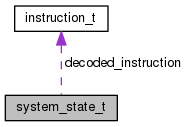
\includegraphics[width=213pt]{structsystem__state__t__coll__graph}
\end{center}
\end{figure}
\subsection*{Data Fields}
\begin{DoxyCompactItemize}
\item 
\hyperlink{global_8h_a0e7744482eed560726581dae7d3cb8b2}{word\+\_\+t} \hyperlink{structsystem__state__t_af042206b1a035449b5a10250fdc29e8f}{registers} \mbox{[}\hyperlink{global_8h_a5efff3a4a48efbf589e3a2320997d9b9}{N\+U\+M\+\_\+\+R\+E\+G\+I\+S\+T\+E\+RS}\mbox{]}
\item 
\hyperlink{global_8h_a0661d7d1353e0bca70c64563f635b034}{byte\+\_\+t} \hyperlink{structsystem__state__t_ade4e6995025b3b8eeeb62bdb38408765}{memory} \mbox{[}\hyperlink{global_8h_ad1d337f69c5203493cb37cb203c33e24}{N\+U\+M\+\_\+\+A\+D\+D\+R\+E\+S\+S\+ES}\mbox{]}
\item 
\hyperlink{global_8h_a0e7744482eed560726581dae7d3cb8b2}{word\+\_\+t} \hyperlink{structsystem__state__t_a9cb73fc3980fae6ad4eff34e8461d947}{fetched\+\_\+instruction}
\item 
\hyperlink{structinstruction__t}{instruction\+\_\+t} $\ast$ \hyperlink{structsystem__state__t_ab53a970384d9c812a2a4c6e327b19a95}{decoded\+\_\+instruction}
\item 
bool \hyperlink{structsystem__state__t_afe188f4e4c4fed3fab882599cfdafa76}{has\+\_\+fetched\+\_\+instruction}
\end{DoxyCompactItemize}


\subsection{Detailed Description}
A struct that holds information about the current system state. 

\subsection{Field Documentation}
\index{system\+\_\+state\+\_\+t@{system\+\_\+state\+\_\+t}!decoded\+\_\+instruction@{decoded\+\_\+instruction}}
\index{decoded\+\_\+instruction@{decoded\+\_\+instruction}!system\+\_\+state\+\_\+t@{system\+\_\+state\+\_\+t}}
\subsubsection[{\texorpdfstring{decoded\+\_\+instruction}{decoded_instruction}}]{\setlength{\rightskip}{0pt plus 5cm}{\bf instruction\+\_\+t}$\ast$ system\+\_\+state\+\_\+t\+::decoded\+\_\+instruction}\hypertarget{structsystem__state__t_ab53a970384d9c812a2a4c6e327b19a95}{}\label{structsystem__state__t_ab53a970384d9c812a2a4c6e327b19a95}
Holds the last decoded instruction, as an \hyperlink{structinstruction__t}{instruction\+\_\+t} type. \index{system\+\_\+state\+\_\+t@{system\+\_\+state\+\_\+t}!fetched\+\_\+instruction@{fetched\+\_\+instruction}}
\index{fetched\+\_\+instruction@{fetched\+\_\+instruction}!system\+\_\+state\+\_\+t@{system\+\_\+state\+\_\+t}}
\subsubsection[{\texorpdfstring{fetched\+\_\+instruction}{fetched_instruction}}]{\setlength{\rightskip}{0pt plus 5cm}{\bf word\+\_\+t} system\+\_\+state\+\_\+t\+::fetched\+\_\+instruction}\hypertarget{structsystem__state__t_a9cb73fc3980fae6ad4eff34e8461d947}{}\label{structsystem__state__t_a9cb73fc3980fae6ad4eff34e8461d947}
Holds the last fetched instruction, as a word. \index{system\+\_\+state\+\_\+t@{system\+\_\+state\+\_\+t}!has\+\_\+fetched\+\_\+instruction@{has\+\_\+fetched\+\_\+instruction}}
\index{has\+\_\+fetched\+\_\+instruction@{has\+\_\+fetched\+\_\+instruction}!system\+\_\+state\+\_\+t@{system\+\_\+state\+\_\+t}}
\subsubsection[{\texorpdfstring{has\+\_\+fetched\+\_\+instruction}{has_fetched_instruction}}]{\setlength{\rightskip}{0pt plus 5cm}bool system\+\_\+state\+\_\+t\+::has\+\_\+fetched\+\_\+instruction}\hypertarget{structsystem__state__t_afe188f4e4c4fed3fab882599cfdafa76}{}\label{structsystem__state__t_afe188f4e4c4fed3fab882599cfdafa76}
Whether or not the system currently has a fetched instruction. \index{system\+\_\+state\+\_\+t@{system\+\_\+state\+\_\+t}!memory@{memory}}
\index{memory@{memory}!system\+\_\+state\+\_\+t@{system\+\_\+state\+\_\+t}}
\subsubsection[{\texorpdfstring{memory}{memory}}]{\setlength{\rightskip}{0pt plus 5cm}{\bf byte\+\_\+t} system\+\_\+state\+\_\+t\+::memory\mbox{[}{\bf N\+U\+M\+\_\+\+A\+D\+D\+R\+E\+S\+S\+ES}\mbox{]}}\hypertarget{structsystem__state__t_ade4e6995025b3b8eeeb62bdb38408765}{}\label{structsystem__state__t_ade4e6995025b3b8eeeb62bdb38408765}
Holds the values currently held in memory. \index{system\+\_\+state\+\_\+t@{system\+\_\+state\+\_\+t}!registers@{registers}}
\index{registers@{registers}!system\+\_\+state\+\_\+t@{system\+\_\+state\+\_\+t}}
\subsubsection[{\texorpdfstring{registers}{registers}}]{\setlength{\rightskip}{0pt plus 5cm}{\bf word\+\_\+t} system\+\_\+state\+\_\+t\+::registers\mbox{[}{\bf N\+U\+M\+\_\+\+R\+E\+G\+I\+S\+T\+E\+RS}\mbox{]}}\hypertarget{structsystem__state__t_af042206b1a035449b5a10250fdc29e8f}{}\label{structsystem__state__t_af042206b1a035449b5a10250fdc29e8f}
Holds the values currently held in registers. 

The documentation for this struct was generated from the following file\+:\begin{DoxyCompactItemize}
\item 
emulate\+\_\+utils/\hyperlink{system__state_8h}{system\+\_\+state.\+h}\end{DoxyCompactItemize}

\hypertarget{structvalue__carry__t}{}\section{value\+\_\+carry\+\_\+t Struct Reference}
\label{structvalue__carry__t}\index{value\+\_\+carry\+\_\+t@{value\+\_\+carry\+\_\+t}}


A struct that has a value and a carry.  




{\ttfamily \#include $<$value\+\_\+carry.\+h$>$}

\subsection*{Data Fields}
\begin{DoxyCompactItemize}
\item 
\hyperlink{global_8h_a0e7744482eed560726581dae7d3cb8b2}{word\+\_\+t} \hyperlink{structvalue__carry__t_a4ee942fb80f5e029be0e70fb36fbe7d2}{value}
\begin{DoxyCompactList}\small\item\em The value. \end{DoxyCompactList}\item 
bool \hyperlink{structvalue__carry__t_acc16f68935549d72338a641a70b7a002}{carry}
\begin{DoxyCompactList}\small\item\em Whether or not there is a carry bit present. \end{DoxyCompactList}\end{DoxyCompactItemize}


\subsection{Detailed Description}
A struct that has a value and a carry. 

\subsection{Field Documentation}
\index{value\+\_\+carry\+\_\+t@{value\+\_\+carry\+\_\+t}!carry@{carry}}
\index{carry@{carry}!value\+\_\+carry\+\_\+t@{value\+\_\+carry\+\_\+t}}
\subsubsection[{\texorpdfstring{carry}{carry}}]{\setlength{\rightskip}{0pt plus 5cm}bool value\+\_\+carry\+\_\+t\+::carry}\hypertarget{structvalue__carry__t_acc16f68935549d72338a641a70b7a002}{}\label{structvalue__carry__t_acc16f68935549d72338a641a70b7a002}


Whether or not there is a carry bit present. 

\index{value\+\_\+carry\+\_\+t@{value\+\_\+carry\+\_\+t}!value@{value}}
\index{value@{value}!value\+\_\+carry\+\_\+t@{value\+\_\+carry\+\_\+t}}
\subsubsection[{\texorpdfstring{value}{value}}]{\setlength{\rightskip}{0pt plus 5cm}{\bf word\+\_\+t} value\+\_\+carry\+\_\+t\+::value}\hypertarget{structvalue__carry__t_a4ee942fb80f5e029be0e70fb36fbe7d2}{}\label{structvalue__carry__t_a4ee942fb80f5e029be0e70fb36fbe7d2}


The value. 



The documentation for this struct was generated from the following file\+:\begin{DoxyCompactItemize}
\item 
\hyperlink{value__carry_8h}{value\+\_\+carry.\+h}\end{DoxyCompactItemize}

\chapter{File Documentation}
\hypertarget{decode_8c}{}\section{emulate\+\_\+utils/decode.c File Reference}
\label{decode_8c}\index{emulate\+\_\+utils/decode.\+c@{emulate\+\_\+utils/decode.\+c}}


Functions for the decode cycle.  


{\ttfamily \#include \char`\"{}decode.\+h\char`\"{}}\\*
Include dependency graph for decode.\+c\+:\nopagebreak
\begin{figure}[H]
\begin{center}
\leavevmode
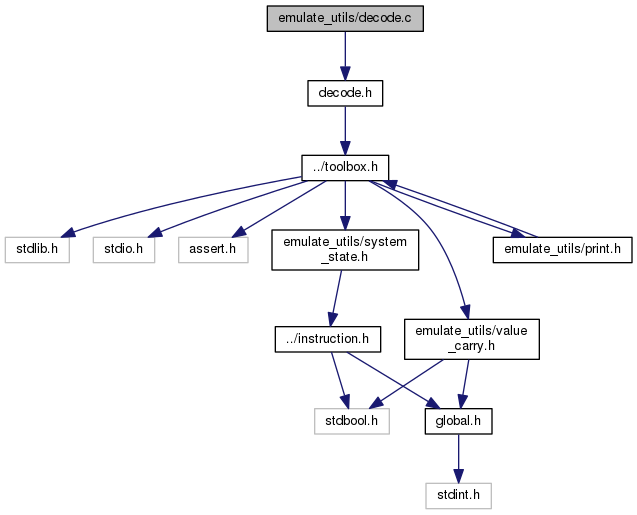
\includegraphics[width=350pt]{decode_8c__incl}
\end{center}
\end{figure}
\subsection*{Functions}
\begin{DoxyCompactItemize}
\item 
void \hyperlink{decode_8c_ab6398a4c7d3377837b94bb0386f062c6}{decode\+\_\+instruction} (\hyperlink{structsystem__state__t}{system\+\_\+state\+\_\+t} $\ast$machine)
\begin{DoxyCompactList}\small\item\em Decodes the fetched instruction in current system state. \end{DoxyCompactList}\item 
void \hyperlink{decode_8c_a3d488112b7f20aa0ab705253c3aa6ec3}{halt} (\hyperlink{structsystem__state__t}{system\+\_\+state\+\_\+t} $\ast$machine)
\begin{DoxyCompactList}\small\item\em Sets decoded\+\_\+instruction type to a stop (Z\+ER) instruction. \end{DoxyCompactList}\item 
void \hyperlink{decode_8c_a2a0f621c80c6894c383548f8dd225f2d}{branch} (\hyperlink{structsystem__state__t}{system\+\_\+state\+\_\+t} $\ast$machine)
\begin{DoxyCompactList}\small\item\em Set branch instruction data in decoded\+\_\+instruction. \end{DoxyCompactList}\item 
void \hyperlink{decode_8c_af5cd2d82cc551d03c65948e27e3dea1d}{multiply} (\hyperlink{structsystem__state__t}{system\+\_\+state\+\_\+t} $\ast$machine)
\begin{DoxyCompactList}\small\item\em Set multiply instruction data in decoded\+\_\+instruction. \end{DoxyCompactList}\item 
void \hyperlink{decode_8c_af5da0fb4f844c3c75f81601b5d648b6f}{single\+\_\+data\+\_\+transfer} (\hyperlink{structsystem__state__t}{system\+\_\+state\+\_\+t} $\ast$machine)
\begin{DoxyCompactList}\small\item\em Set single\+\_\+data\+\_\+transfer instruction data in decoded\+\_\+instruction. \end{DoxyCompactList}\item 
void \hyperlink{decode_8c_a7f2d97f06ba3dcb9b484decf650c5067}{data\+\_\+processing} (\hyperlink{structsystem__state__t}{system\+\_\+state\+\_\+t} $\ast$machine)
\begin{DoxyCompactList}\small\item\em Set data\+\_\+processing instruction data in decoded\+\_\+instruction. \end{DoxyCompactList}\end{DoxyCompactItemize}


\subsection{Detailed Description}
Functions for the decode cycle. 



\subsection{Function Documentation}
\index{decode.\+c@{decode.\+c}!branch@{branch}}
\index{branch@{branch}!decode.\+c@{decode.\+c}}
\subsubsection[{\texorpdfstring{branch(system\+\_\+state\+\_\+t $\ast$machine)}{branch(system_state_t *machine)}}]{\setlength{\rightskip}{0pt plus 5cm}void branch (
\begin{DoxyParamCaption}
\item[{{\bf system\+\_\+state\+\_\+t} $\ast$}]{machine}
\end{DoxyParamCaption}
)}\hypertarget{decode_8c_a2a0f621c80c6894c383548f8dd225f2d}{}\label{decode_8c_a2a0f621c80c6894c383548f8dd225f2d}


Set branch instruction data in decoded\+\_\+instruction. 

The offset (24 bits) is bit 0 to 23 of the branch instruction. It is then bit shifted to the left by 2 and then sign extended to 32 bits. The offset is stored in the immediate\+\_\+value of the decoded\+\_\+instruction. 
\begin{DoxyParams}{Parameters}
{\em machine} & The current system state. \\
\hline
\end{DoxyParams}
\index{decode.\+c@{decode.\+c}!data\+\_\+processing@{data\+\_\+processing}}
\index{data\+\_\+processing@{data\+\_\+processing}!decode.\+c@{decode.\+c}}
\subsubsection[{\texorpdfstring{data\+\_\+processing(system\+\_\+state\+\_\+t $\ast$machine)}{data_processing(system_state_t *machine)}}]{\setlength{\rightskip}{0pt plus 5cm}void data\+\_\+processing (
\begin{DoxyParamCaption}
\item[{{\bf system\+\_\+state\+\_\+t} $\ast$}]{machine}
\end{DoxyParamCaption}
)}\hypertarget{decode_8c_a7f2d97f06ba3dcb9b484decf650c5067}{}\label{decode_8c_a7f2d97f06ba3dcb9b484decf650c5067}


Set data\+\_\+processing instruction data in decoded\+\_\+instruction. 

The fields in decoded\+\_\+instruction are used as follows\+:
\begin{DoxyItemize}
\item flag\+\_\+0 stores the I bit\+:
\begin{DoxyItemize}
\item If set, the Operand2 is used as an immediate constant.
\item Otherwise, Operand2 is used as a shifted register.
\end{DoxyItemize}
\item flag\+\_\+1 stores the S bit (if set, C\+P\+SR flags are set when executed).
\item operation is used to store the corresponding opcode\+\_\+t enum to the opcode. provided in the fetched\+\_\+instruction.
\item rd is the source/destination register address.
\item rn is the first operand register. 
\begin{DoxyParams}{Parameters}
{\em machine} & The current system state. \\
\hline
\end{DoxyParams}

\end{DoxyItemize}\index{decode.\+c@{decode.\+c}!decode\+\_\+instruction@{decode\+\_\+instruction}}
\index{decode\+\_\+instruction@{decode\+\_\+instruction}!decode.\+c@{decode.\+c}}
\subsubsection[{\texorpdfstring{decode\+\_\+instruction(system\+\_\+state\+\_\+t $\ast$machine)}{decode_instruction(system_state_t *machine)}}]{\setlength{\rightskip}{0pt plus 5cm}void decode\+\_\+instruction (
\begin{DoxyParamCaption}
\item[{{\bf system\+\_\+state\+\_\+t} $\ast$}]{machine}
\end{DoxyParamCaption}
)}\hypertarget{decode_8c_ab6398a4c7d3377837b94bb0386f062c6}{}\label{decode_8c_ab6398a4c7d3377837b94bb0386f062c6}


Decodes the fetched instruction in current system state. 

Given the pointer to the current system state, it moves the fetched instruction information into the decoded\+\_\+instruction struct (for use when executing the decoded instruction). 
\begin{DoxyParams}{Parameters}
{\em machine} & The current system state. \\
\hline
\end{DoxyParams}
\index{decode.\+c@{decode.\+c}!halt@{halt}}
\index{halt@{halt}!decode.\+c@{decode.\+c}}
\subsubsection[{\texorpdfstring{halt(system\+\_\+state\+\_\+t $\ast$machine)}{halt(system_state_t *machine)}}]{\setlength{\rightskip}{0pt plus 5cm}void halt (
\begin{DoxyParamCaption}
\item[{{\bf system\+\_\+state\+\_\+t} $\ast$}]{machine}
\end{DoxyParamCaption}
)}\hypertarget{decode_8c_a3d488112b7f20aa0ab705253c3aa6ec3}{}\label{decode_8c_a3d488112b7f20aa0ab705253c3aa6ec3}


Sets decoded\+\_\+instruction type to a stop (Z\+ER) instruction. 


\begin{DoxyParams}{Parameters}
{\em machine} & The current system state. \\
\hline
\end{DoxyParams}
\index{decode.\+c@{decode.\+c}!multiply@{multiply}}
\index{multiply@{multiply}!decode.\+c@{decode.\+c}}
\subsubsection[{\texorpdfstring{multiply(system\+\_\+state\+\_\+t $\ast$machine)}{multiply(system_state_t *machine)}}]{\setlength{\rightskip}{0pt plus 5cm}void multiply (
\begin{DoxyParamCaption}
\item[{{\bf system\+\_\+state\+\_\+t} $\ast$}]{machine}
\end{DoxyParamCaption}
)}\hypertarget{decode_8c_af5cd2d82cc551d03c65948e27e3dea1d}{}\label{decode_8c_af5cd2d82cc551d03c65948e27e3dea1d}


Set multiply instruction data in decoded\+\_\+instruction. 

The fields in decoded\+\_\+instruction are used as follows\+:
\begin{DoxyItemize}
\item flag\+\_\+0 stores the A bit (if set, perform multiply and accumulate).
\item flag\+\_\+1 stores the S bit (if set, C\+P\+SR flags are set when executed).
\item rd is the destination register address.
\item rn, rs and rm are the addresses of the operand registers. 
\begin{DoxyParams}{Parameters}
{\em machine} & The current system state. \\
\hline
\end{DoxyParams}

\end{DoxyItemize}\index{decode.\+c@{decode.\+c}!single\+\_\+data\+\_\+transfer@{single\+\_\+data\+\_\+transfer}}
\index{single\+\_\+data\+\_\+transfer@{single\+\_\+data\+\_\+transfer}!decode.\+c@{decode.\+c}}
\subsubsection[{\texorpdfstring{single\+\_\+data\+\_\+transfer(system\+\_\+state\+\_\+t $\ast$machine)}{single_data_transfer(system_state_t *machine)}}]{\setlength{\rightskip}{0pt plus 5cm}void single\+\_\+data\+\_\+transfer (
\begin{DoxyParamCaption}
\item[{{\bf system\+\_\+state\+\_\+t} $\ast$}]{machine}
\end{DoxyParamCaption}
)}\hypertarget{decode_8c_af5da0fb4f844c3c75f81601b5d648b6f}{}\label{decode_8c_af5da0fb4f844c3c75f81601b5d648b6f}


Set single\+\_\+data\+\_\+transfer instruction data in decoded\+\_\+instruction. 

The fields in decoded\+\_\+instruction are used as follows\+:
\begin{DoxyItemize}
\item flag\+\_\+0 stores the I bit\+:
\begin{DoxyItemize}
\item If set, Offset is used as a shifted register.
\item Otherwise, Offset is used as an unsigned 12 bit immediate offset).
\end{DoxyItemize}
\item flag\+\_\+1 stores the P bit\+:
\begin{DoxyItemize}
\item If set, pre-\/indexing is used.
\item Otherwise, post-\/indexing is used.
\end{DoxyItemize}
\item flag\+\_\+2 stores the U bit\+:
\begin{DoxyItemize}
\item If set, Offset is added to the base register.
\item Otherwise, Offset is subtracted from the base register.
\end{DoxyItemize}
\item flag\+\_\+3 stores the L bit\+:
\begin{DoxyItemize}
\item If set, the word is loaded from memory.
\item Otherwise, the word is stored into memory.
\end{DoxyItemize}
\item rd is the source/destination register address.
\item rn is the base register. 
\begin{DoxyParams}{Parameters}
{\em machine} & The current system state. \\
\hline
\end{DoxyParams}

\end{DoxyItemize}
\hypertarget{decode_8h}{}\section{emulate\+\_\+utils/decode.h File Reference}
\label{decode_8h}\index{emulate\+\_\+utils/decode.\+h@{emulate\+\_\+utils/decode.\+h}}


Header file for \hyperlink{decode_8c}{decode.\+c}.  


{\ttfamily \#include \char`\"{}../toolbox.\+h\char`\"{}}\\*
Include dependency graph for decode.\+h\+:\nopagebreak
\begin{figure}[H]
\begin{center}
\leavevmode
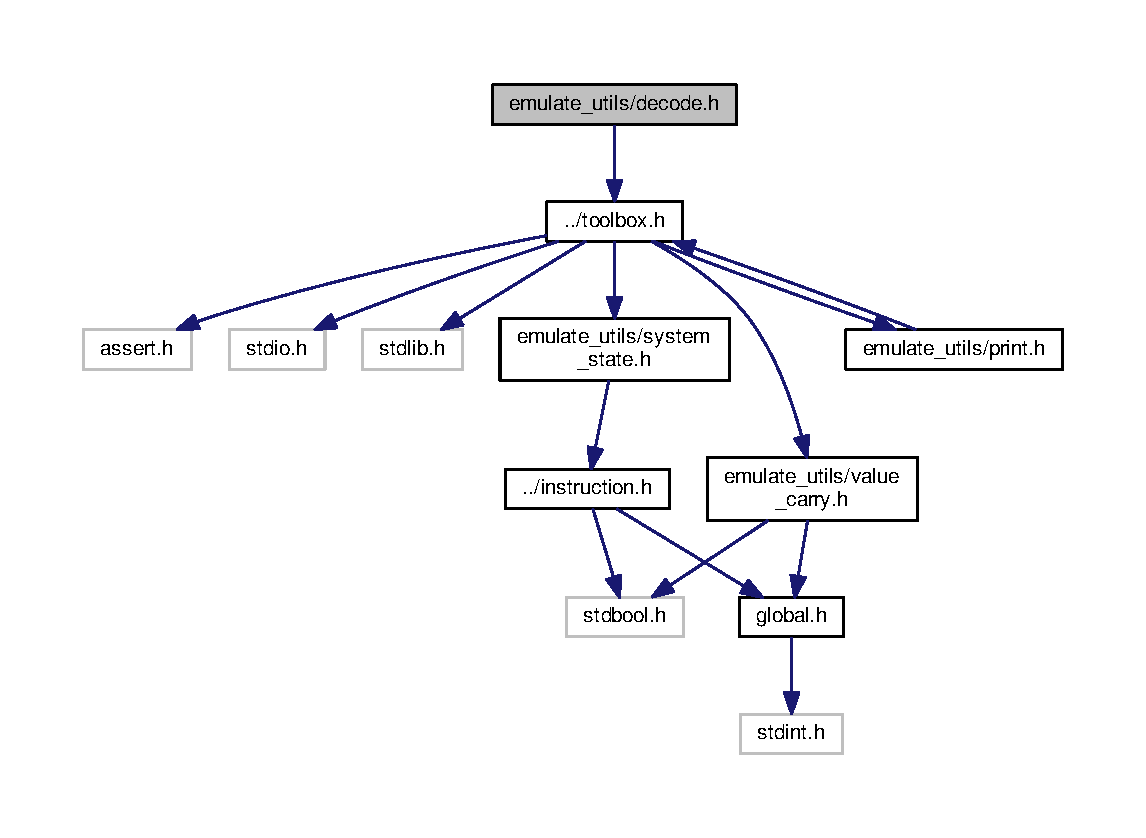
\includegraphics[width=350pt]{decode_8h__incl}
\end{center}
\end{figure}
This graph shows which files directly or indirectly include this file\+:\nopagebreak
\begin{figure}[H]
\begin{center}
\leavevmode
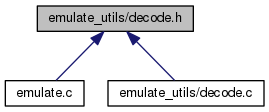
\includegraphics[width=274pt]{decode_8h__dep__incl}
\end{center}
\end{figure}
\subsection*{Functions}
\begin{DoxyCompactItemize}
\item 
void \hyperlink{decode_8h_ab6398a4c7d3377837b94bb0386f062c6}{decode\+\_\+instruction} (\hyperlink{structsystem__state__t}{system\+\_\+state\+\_\+t} $\ast$machine)
\begin{DoxyCompactList}\small\item\em Decodes the fetched instruction in current system state. \end{DoxyCompactList}\item 
void \hyperlink{decode_8h_a3d488112b7f20aa0ab705253c3aa6ec3}{halt} (\hyperlink{structsystem__state__t}{system\+\_\+state\+\_\+t} $\ast$machine)
\begin{DoxyCompactList}\small\item\em Sets decoded\+\_\+instruction type to a stop (Z\+ER) instruction. \end{DoxyCompactList}\item 
void \hyperlink{decode_8h_a2a0f621c80c6894c383548f8dd225f2d}{branch} (\hyperlink{structsystem__state__t}{system\+\_\+state\+\_\+t} $\ast$machine)
\begin{DoxyCompactList}\small\item\em Set branch instruction data in decoded\+\_\+instruction. \end{DoxyCompactList}\item 
void \hyperlink{decode_8h_af5da0fb4f844c3c75f81601b5d648b6f}{single\+\_\+data\+\_\+transfer} (\hyperlink{structsystem__state__t}{system\+\_\+state\+\_\+t} $\ast$machine)
\begin{DoxyCompactList}\small\item\em Set single\+\_\+data\+\_\+transfer instruction data in decoded\+\_\+instruction. \end{DoxyCompactList}\item 
void \hyperlink{decode_8h_af5cd2d82cc551d03c65948e27e3dea1d}{multiply} (\hyperlink{structsystem__state__t}{system\+\_\+state\+\_\+t} $\ast$machine)
\begin{DoxyCompactList}\small\item\em Set multiply instruction data in decoded\+\_\+instruction. \end{DoxyCompactList}\item 
void \hyperlink{decode_8h_a7f2d97f06ba3dcb9b484decf650c5067}{data\+\_\+processing} (\hyperlink{structsystem__state__t}{system\+\_\+state\+\_\+t} $\ast$machine)
\begin{DoxyCompactList}\small\item\em Set data\+\_\+processing instruction data in decoded\+\_\+instruction. \end{DoxyCompactList}\end{DoxyCompactItemize}


\subsection{Detailed Description}
Header file for \hyperlink{decode_8c}{decode.\+c}. 



\subsection{Function Documentation}
\index{decode.\+h@{decode.\+h}!branch@{branch}}
\index{branch@{branch}!decode.\+h@{decode.\+h}}
\subsubsection[{\texorpdfstring{branch(system\+\_\+state\+\_\+t $\ast$machine)}{branch(system_state_t *machine)}}]{\setlength{\rightskip}{0pt plus 5cm}void branch (
\begin{DoxyParamCaption}
\item[{{\bf system\+\_\+state\+\_\+t} $\ast$}]{machine}
\end{DoxyParamCaption}
)}\hypertarget{decode_8h_a2a0f621c80c6894c383548f8dd225f2d}{}\label{decode_8h_a2a0f621c80c6894c383548f8dd225f2d}


Set branch instruction data in decoded\+\_\+instruction. 

The offset (24 bits) is bit 0 to 23 of the branch instruction. It is then bit shifted to the left by 2 and then sign extended to 32 bits. The offset is stored in the immediate\+\_\+value of the decoded\+\_\+instruction. 
\begin{DoxyParams}{Parameters}
{\em machine} & The current system state. \\
\hline
\end{DoxyParams}
\index{decode.\+h@{decode.\+h}!data\+\_\+processing@{data\+\_\+processing}}
\index{data\+\_\+processing@{data\+\_\+processing}!decode.\+h@{decode.\+h}}
\subsubsection[{\texorpdfstring{data\+\_\+processing(system\+\_\+state\+\_\+t $\ast$machine)}{data_processing(system_state_t *machine)}}]{\setlength{\rightskip}{0pt plus 5cm}void data\+\_\+processing (
\begin{DoxyParamCaption}
\item[{{\bf system\+\_\+state\+\_\+t} $\ast$}]{machine}
\end{DoxyParamCaption}
)}\hypertarget{decode_8h_a7f2d97f06ba3dcb9b484decf650c5067}{}\label{decode_8h_a7f2d97f06ba3dcb9b484decf650c5067}


Set data\+\_\+processing instruction data in decoded\+\_\+instruction. 

The fields in decoded\+\_\+instruction are used as follows\+:
\begin{DoxyItemize}
\item flag\+\_\+0 stores the I bit\+:
\begin{DoxyItemize}
\item If set, the Operand2 is used as an immediate constant.
\item Otherwise, Operand2 is used as a shifted register.
\end{DoxyItemize}
\item flag\+\_\+1 stores the S bit (if set, C\+P\+SR flags are set when executed).
\item operation is used to store the corresponding opcode\+\_\+t enum to the opcode. provided in the fetched\+\_\+instruction.
\item rd is the source/destination register address.
\item rn is the first operand register. 
\begin{DoxyParams}{Parameters}
{\em machine} & The current system state. \\
\hline
\end{DoxyParams}

\end{DoxyItemize}\index{decode.\+h@{decode.\+h}!decode\+\_\+instruction@{decode\+\_\+instruction}}
\index{decode\+\_\+instruction@{decode\+\_\+instruction}!decode.\+h@{decode.\+h}}
\subsubsection[{\texorpdfstring{decode\+\_\+instruction(system\+\_\+state\+\_\+t $\ast$machine)}{decode_instruction(system_state_t *machine)}}]{\setlength{\rightskip}{0pt plus 5cm}void decode\+\_\+instruction (
\begin{DoxyParamCaption}
\item[{{\bf system\+\_\+state\+\_\+t} $\ast$}]{machine}
\end{DoxyParamCaption}
)}\hypertarget{decode_8h_ab6398a4c7d3377837b94bb0386f062c6}{}\label{decode_8h_ab6398a4c7d3377837b94bb0386f062c6}


Decodes the fetched instruction in current system state. 

Given the pointer to the current system state, it moves the fetched instruction information into the decoded\+\_\+instruction struct (for use when executing the decoded instruction). 
\begin{DoxyParams}{Parameters}
{\em machine} & The current system state. \\
\hline
\end{DoxyParams}
\index{decode.\+h@{decode.\+h}!halt@{halt}}
\index{halt@{halt}!decode.\+h@{decode.\+h}}
\subsubsection[{\texorpdfstring{halt(system\+\_\+state\+\_\+t $\ast$machine)}{halt(system_state_t *machine)}}]{\setlength{\rightskip}{0pt plus 5cm}void halt (
\begin{DoxyParamCaption}
\item[{{\bf system\+\_\+state\+\_\+t} $\ast$}]{machine}
\end{DoxyParamCaption}
)}\hypertarget{decode_8h_a3d488112b7f20aa0ab705253c3aa6ec3}{}\label{decode_8h_a3d488112b7f20aa0ab705253c3aa6ec3}


Sets decoded\+\_\+instruction type to a stop (Z\+ER) instruction. 


\begin{DoxyParams}{Parameters}
{\em machine} & The current system state. \\
\hline
\end{DoxyParams}
\index{decode.\+h@{decode.\+h}!multiply@{multiply}}
\index{multiply@{multiply}!decode.\+h@{decode.\+h}}
\subsubsection[{\texorpdfstring{multiply(system\+\_\+state\+\_\+t $\ast$machine)}{multiply(system_state_t *machine)}}]{\setlength{\rightskip}{0pt plus 5cm}void multiply (
\begin{DoxyParamCaption}
\item[{{\bf system\+\_\+state\+\_\+t} $\ast$}]{machine}
\end{DoxyParamCaption}
)}\hypertarget{decode_8h_af5cd2d82cc551d03c65948e27e3dea1d}{}\label{decode_8h_af5cd2d82cc551d03c65948e27e3dea1d}


Set multiply instruction data in decoded\+\_\+instruction. 

The fields in decoded\+\_\+instruction are used as follows\+:
\begin{DoxyItemize}
\item flag\+\_\+0 stores the A bit (if set, perform multiply and accumulate).
\item flag\+\_\+1 stores the S bit (if set, C\+P\+SR flags are set when executed).
\item rd is the destination register address.
\item rn, rs and rm are the addresses of the operand registers. 
\begin{DoxyParams}{Parameters}
{\em machine} & The current system state. \\
\hline
\end{DoxyParams}

\end{DoxyItemize}\index{decode.\+h@{decode.\+h}!single\+\_\+data\+\_\+transfer@{single\+\_\+data\+\_\+transfer}}
\index{single\+\_\+data\+\_\+transfer@{single\+\_\+data\+\_\+transfer}!decode.\+h@{decode.\+h}}
\subsubsection[{\texorpdfstring{single\+\_\+data\+\_\+transfer(system\+\_\+state\+\_\+t $\ast$machine)}{single_data_transfer(system_state_t *machine)}}]{\setlength{\rightskip}{0pt plus 5cm}void single\+\_\+data\+\_\+transfer (
\begin{DoxyParamCaption}
\item[{{\bf system\+\_\+state\+\_\+t} $\ast$}]{machine}
\end{DoxyParamCaption}
)}\hypertarget{decode_8h_af5da0fb4f844c3c75f81601b5d648b6f}{}\label{decode_8h_af5da0fb4f844c3c75f81601b5d648b6f}


Set single\+\_\+data\+\_\+transfer instruction data in decoded\+\_\+instruction. 

The fields in decoded\+\_\+instruction are used as follows\+:
\begin{DoxyItemize}
\item flag\+\_\+0 stores the I bit\+:
\begin{DoxyItemize}
\item If set, Offset is used as a shifted register.
\item Otherwise, Offset is used as an unsigned 12 bit immediate offset).
\end{DoxyItemize}
\item flag\+\_\+1 stores the P bit\+:
\begin{DoxyItemize}
\item If set, pre-\/indexing is used.
\item Otherwise, post-\/indexing is used.
\end{DoxyItemize}
\item flag\+\_\+2 stores the U bit\+:
\begin{DoxyItemize}
\item If set, Offset is added to the base register.
\item Otherwise, Offset is subtracted from the base register.
\end{DoxyItemize}
\item flag\+\_\+3 stores the L bit\+:
\begin{DoxyItemize}
\item If set, the word is loaded from memory.
\item Otherwise, the word is stored into memory.
\end{DoxyItemize}
\item rd is the source/destination register address.
\item rn is the base register. 
\begin{DoxyParams}{Parameters}
{\em machine} & The current system state. \\
\hline
\end{DoxyParams}

\end{DoxyItemize}
\hypertarget{emulate_8c}{}\section{emulate.\+c File Reference}
\label{emulate_8c}\index{emulate.\+c@{emulate.\+c}}


The main functionality for the A\+R\+M11 emulator.  


{\ttfamily \#include \char`\"{}emulate\+\_\+utils/decode.\+h\char`\"{}}\\*
{\ttfamily \#include \char`\"{}emulate\+\_\+utils/execute.\+h\char`\"{}}\\*
{\ttfamily \#include \char`\"{}emulate\+\_\+utils/print\+\_\+compliant.\+h\char`\"{}}\\*
Include dependency graph for emulate.\+c\+:
\nopagebreak
\begin{figure}[H]
\begin{center}
\leavevmode
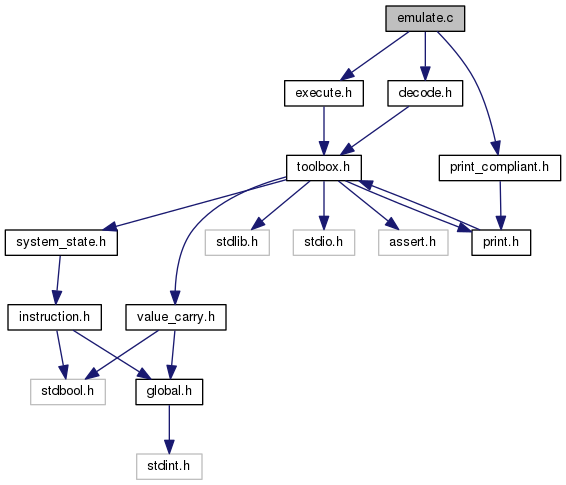
\includegraphics[width=350pt]{emulate_8c__incl}
\end{center}
\end{figure}
\subsection*{Functions}
\begin{DoxyCompactItemize}
\item 
int \hyperlink{emulate_8c_a3c04138a5bfe5d72780bb7e82a18e627}{main} (int argc, char $\ast$$\ast$argv)
\begin{DoxyCompactList}\small\item\em Emulates an A\+R\+M11 machine operating on a given binary file. \end{DoxyCompactList}\end{DoxyCompactItemize}


\subsection{Detailed Description}
The main functionality for the A\+R\+M11 emulator. 



\subsection{Function Documentation}
\index{emulate.\+c@{emulate.\+c}!main@{main}}
\index{main@{main}!emulate.\+c@{emulate.\+c}}
\subsubsection[{\texorpdfstring{main(int argc, char $\ast$$\ast$argv)}{main(int argc, char **argv)}}]{\setlength{\rightskip}{0pt plus 5cm}int main (
\begin{DoxyParamCaption}
\item[{int}]{argc, }
\item[{char $\ast$$\ast$}]{argv}
\end{DoxyParamCaption}
)}\hypertarget{emulate_8c_a3c04138a5bfe5d72780bb7e82a18e627}{}\label{emulate_8c_a3c04138a5bfe5d72780bb7e82a18e627}


Emulates an A\+R\+M11 machine operating on a given binary file. 

The user must provide a single argument, which is a valid file name for an A\+R\+M11 binary object code file. This function emulates the A\+RM architecture, returning details of the registers and non-\/zero memory at the end of execution. 
\hypertarget{execute_8c}{}\section{execute.\+c File Reference}
\label{execute_8c}\index{execute.\+c@{execute.\+c}}


Functions for the execute cycle.  


{\ttfamily \#include \char`\"{}execute.\+h\char`\"{}}\\*
Include dependency graph for execute.\+c\+:
\nopagebreak
\begin{figure}[H]
\begin{center}
\leavevmode
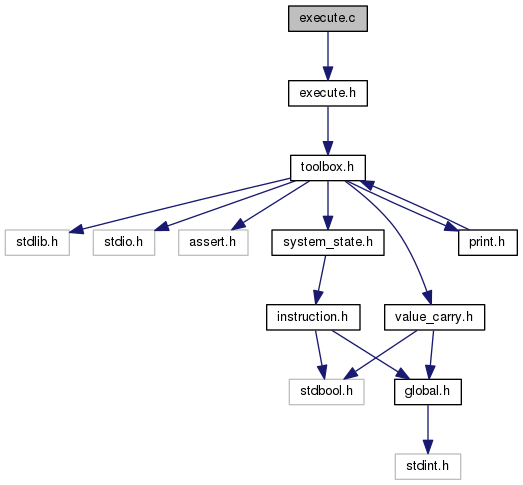
\includegraphics[width=350pt]{execute_8c__incl}
\end{center}
\end{figure}
\subsection*{Functions}
\begin{DoxyCompactItemize}
\item 
int \hyperlink{execute_8c_a5cc462b6d65eef64aaf4600e1b12d5a1}{condition} (\hyperlink{structsystem__state__t}{system\+\_\+state\+\_\+t} $\ast$machine)
\begin{DoxyCompactList}\small\item\em Returns whether the condition is met. \end{DoxyCompactList}\item 
void \hyperlink{execute_8c_a31c5a2d2e957a126e3e1dc7e57719321}{execute} (\hyperlink{structsystem__state__t}{system\+\_\+state\+\_\+t} $\ast$machine)
\begin{DoxyCompactList}\small\item\em Runs one execute cycle. \end{DoxyCompactList}\item 
void \hyperlink{execute_8c_a9e2db6093fbac9addda00ff4486a1144}{execute\+\_\+dpi} (\hyperlink{structsystem__state__t}{system\+\_\+state\+\_\+t} $\ast$machine)
\begin{DoxyCompactList}\small\item\em Executes a data processing instruction. \end{DoxyCompactList}\item 
void \hyperlink{execute_8c_a7945df503581748ddca5f2e4ebee0332}{execute\+\_\+mul} (\hyperlink{structsystem__state__t}{system\+\_\+state\+\_\+t} $\ast$machine)
\begin{DoxyCompactList}\small\item\em Executes a multiply instruction. \end{DoxyCompactList}\item 
void \hyperlink{execute_8c_a86977d43b2a9ac022bab66ecc71e7e8a}{execute\+\_\+sdt} (\hyperlink{structsystem__state__t}{system\+\_\+state\+\_\+t} $\ast$machine)
\begin{DoxyCompactList}\small\item\em Executes a single data transfer instruction. \end{DoxyCompactList}\item 
void \hyperlink{execute_8c_a7ae1d45a6401a9009b155ebf5d1f734d}{execute\+\_\+branch} (\hyperlink{structsystem__state__t}{system\+\_\+state\+\_\+t} $\ast$machine)
\begin{DoxyCompactList}\small\item\em Executes a branch instruction. \end{DoxyCompactList}\end{DoxyCompactItemize}


\subsection{Detailed Description}
Functions for the execute cycle. 



\subsection{Function Documentation}
\index{execute.\+c@{execute.\+c}!condition@{condition}}
\index{condition@{condition}!execute.\+c@{execute.\+c}}
\subsubsection[{\texorpdfstring{condition(system\+\_\+state\+\_\+t $\ast$machine)}{condition(system_state_t *machine)}}]{\setlength{\rightskip}{0pt plus 5cm}int condition (
\begin{DoxyParamCaption}
\item[{{\bf system\+\_\+state\+\_\+t} $\ast$}]{machine}
\end{DoxyParamCaption}
)}\hypertarget{execute_8c_a5cc462b6d65eef64aaf4600e1b12d5a1}{}\label{execute_8c_a5cc462b6d65eef64aaf4600e1b12d5a1}


Returns whether the condition is met. 

Returns true if and only if the condition required by the current decoded instruction is met by the current state of the flags register (C\+P\+SR). 
\begin{DoxyParams}{Parameters}
{\em machine} & The current system state. \\
\hline
\end{DoxyParams}
\begin{DoxyReturn}{Returns}
Whether condition is met. 
\end{DoxyReturn}
\index{execute.\+c@{execute.\+c}!execute@{execute}}
\index{execute@{execute}!execute.\+c@{execute.\+c}}
\subsubsection[{\texorpdfstring{execute(system\+\_\+state\+\_\+t $\ast$machine)}{execute(system_state_t *machine)}}]{\setlength{\rightskip}{0pt plus 5cm}void execute (
\begin{DoxyParamCaption}
\item[{{\bf system\+\_\+state\+\_\+t} $\ast$}]{machine}
\end{DoxyParamCaption}
)}\hypertarget{execute_8c_a31c5a2d2e957a126e3e1dc7e57719321}{}\label{execute_8c_a31c5a2d2e957a126e3e1dc7e57719321}


Runs one execute cycle. 

Executes the current decoded instruction if the condition is met, and updates the system state accordingly. A pre-\/condition is that the instruction must not be type N\+UL or Z\+ER. 
\begin{DoxyParams}{Parameters}
{\em machine} & The current system state. \\
\hline
\end{DoxyParams}
\index{execute.\+c@{execute.\+c}!execute\+\_\+branch@{execute\+\_\+branch}}
\index{execute\+\_\+branch@{execute\+\_\+branch}!execute.\+c@{execute.\+c}}
\subsubsection[{\texorpdfstring{execute\+\_\+branch(system\+\_\+state\+\_\+t $\ast$machine)}{execute_branch(system_state_t *machine)}}]{\setlength{\rightskip}{0pt plus 5cm}void execute\+\_\+branch (
\begin{DoxyParamCaption}
\item[{{\bf system\+\_\+state\+\_\+t} $\ast$}]{machine}
\end{DoxyParamCaption}
)}\hypertarget{execute_8c_a7ae1d45a6401a9009b155ebf5d1f734d}{}\label{execute_8c_a7ae1d45a6401a9009b155ebf5d1f734d}


Executes a branch instruction. 


\begin{DoxyParams}{Parameters}
{\em machine} & The current system state. \\
\hline
\end{DoxyParams}
\index{execute.\+c@{execute.\+c}!execute\+\_\+dpi@{execute\+\_\+dpi}}
\index{execute\+\_\+dpi@{execute\+\_\+dpi}!execute.\+c@{execute.\+c}}
\subsubsection[{\texorpdfstring{execute\+\_\+dpi(system\+\_\+state\+\_\+t $\ast$machine)}{execute_dpi(system_state_t *machine)}}]{\setlength{\rightskip}{0pt plus 5cm}void execute\+\_\+dpi (
\begin{DoxyParamCaption}
\item[{{\bf system\+\_\+state\+\_\+t} $\ast$}]{machine}
\end{DoxyParamCaption}
)}\hypertarget{execute_8c_a9e2db6093fbac9addda00ff4486a1144}{}\label{execute_8c_a9e2db6093fbac9addda00ff4486a1144}


Executes a data processing instruction. 


\begin{DoxyParams}{Parameters}
{\em machine} & The current system state. \\
\hline
\end{DoxyParams}
\index{execute.\+c@{execute.\+c}!execute\+\_\+mul@{execute\+\_\+mul}}
\index{execute\+\_\+mul@{execute\+\_\+mul}!execute.\+c@{execute.\+c}}
\subsubsection[{\texorpdfstring{execute\+\_\+mul(system\+\_\+state\+\_\+t $\ast$machine)}{execute_mul(system_state_t *machine)}}]{\setlength{\rightskip}{0pt plus 5cm}void execute\+\_\+mul (
\begin{DoxyParamCaption}
\item[{{\bf system\+\_\+state\+\_\+t} $\ast$}]{machine}
\end{DoxyParamCaption}
)}\hypertarget{execute_8c_a7945df503581748ddca5f2e4ebee0332}{}\label{execute_8c_a7945df503581748ddca5f2e4ebee0332}


Executes a multiply instruction. 


\begin{DoxyParams}{Parameters}
{\em machine} & The current system state. \\
\hline
\end{DoxyParams}
\index{execute.\+c@{execute.\+c}!execute\+\_\+sdt@{execute\+\_\+sdt}}
\index{execute\+\_\+sdt@{execute\+\_\+sdt}!execute.\+c@{execute.\+c}}
\subsubsection[{\texorpdfstring{execute\+\_\+sdt(system\+\_\+state\+\_\+t $\ast$machine)}{execute_sdt(system_state_t *machine)}}]{\setlength{\rightskip}{0pt plus 5cm}void execute\+\_\+sdt (
\begin{DoxyParamCaption}
\item[{{\bf system\+\_\+state\+\_\+t} $\ast$}]{machine}
\end{DoxyParamCaption}
)}\hypertarget{execute_8c_a86977d43b2a9ac022bab66ecc71e7e8a}{}\label{execute_8c_a86977d43b2a9ac022bab66ecc71e7e8a}


Executes a single data transfer instruction. 


\begin{DoxyParams}{Parameters}
{\em machine} & The current system state. \\
\hline
\end{DoxyParams}

\hypertarget{execute_8h}{}\section{emulate\+\_\+utils/execute.h File Reference}
\label{execute_8h}\index{emulate\+\_\+utils/execute.\+h@{emulate\+\_\+utils/execute.\+h}}


Header file for \hyperlink{execute_8c}{execute.\+c}.  


{\ttfamily \#include \char`\"{}../toolbox.\+h\char`\"{}}\\*
Include dependency graph for execute.\+h\+:\nopagebreak
\begin{figure}[H]
\begin{center}
\leavevmode
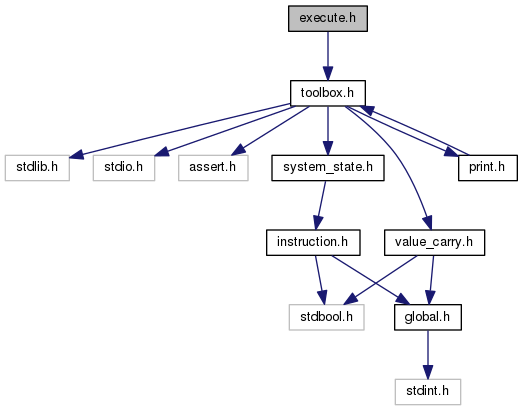
\includegraphics[width=350pt]{execute_8h__incl}
\end{center}
\end{figure}
This graph shows which files directly or indirectly include this file\+:\nopagebreak
\begin{figure}[H]
\begin{center}
\leavevmode
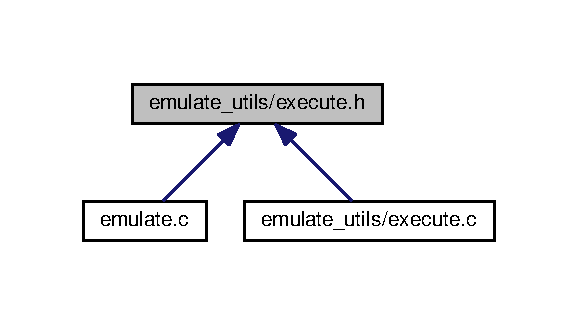
\includegraphics[width=278pt]{execute_8h__dep__incl}
\end{center}
\end{figure}
\subsection*{Functions}
\begin{DoxyCompactItemize}
\item 
void \hyperlink{execute_8h_a31c5a2d2e957a126e3e1dc7e57719321}{execute} (\hyperlink{structsystem__state__t}{system\+\_\+state\+\_\+t} $\ast$machine)
\begin{DoxyCompactList}\small\item\em Runs one execute cycle. \end{DoxyCompactList}\item 
void \hyperlink{execute_8h_a9e2db6093fbac9addda00ff4486a1144}{execute\+\_\+dpi} (\hyperlink{structsystem__state__t}{system\+\_\+state\+\_\+t} $\ast$machine)
\begin{DoxyCompactList}\small\item\em Executes a data processing instruction. \end{DoxyCompactList}\item 
void \hyperlink{execute_8h_a7945df503581748ddca5f2e4ebee0332}{execute\+\_\+mul} (\hyperlink{structsystem__state__t}{system\+\_\+state\+\_\+t} $\ast$machine)
\begin{DoxyCompactList}\small\item\em Executes a multiply instruction. \end{DoxyCompactList}\item 
void \hyperlink{execute_8h_a7ae1d45a6401a9009b155ebf5d1f734d}{execute\+\_\+branch} (\hyperlink{structsystem__state__t}{system\+\_\+state\+\_\+t} $\ast$machine)
\begin{DoxyCompactList}\small\item\em Executes a branch instruction. \end{DoxyCompactList}\item 
void \hyperlink{execute_8h_a86977d43b2a9ac022bab66ecc71e7e8a}{execute\+\_\+sdt} (\hyperlink{structsystem__state__t}{system\+\_\+state\+\_\+t} $\ast$machine)
\begin{DoxyCompactList}\small\item\em Executes a single data transfer instruction. \end{DoxyCompactList}\end{DoxyCompactItemize}


\subsection{Detailed Description}
Header file for \hyperlink{execute_8c}{execute.\+c}. 



\subsection{Function Documentation}
\index{execute.\+h@{execute.\+h}!execute@{execute}}
\index{execute@{execute}!execute.\+h@{execute.\+h}}
\subsubsection[{\texorpdfstring{execute(system\+\_\+state\+\_\+t $\ast$machine)}{execute(system_state_t *machine)}}]{\setlength{\rightskip}{0pt plus 5cm}void execute (
\begin{DoxyParamCaption}
\item[{{\bf system\+\_\+state\+\_\+t} $\ast$}]{machine}
\end{DoxyParamCaption}
)}\hypertarget{execute_8h_a31c5a2d2e957a126e3e1dc7e57719321}{}\label{execute_8h_a31c5a2d2e957a126e3e1dc7e57719321}


Runs one execute cycle. 

Executes the current decoded instruction if the condition is met, and updates the system state accordingly. A pre-\/condition is that the instruction must not be type N\+UL or Z\+ER. 
\begin{DoxyParams}{Parameters}
{\em machine} & The current system state. \\
\hline
\end{DoxyParams}
\index{execute.\+h@{execute.\+h}!execute\+\_\+branch@{execute\+\_\+branch}}
\index{execute\+\_\+branch@{execute\+\_\+branch}!execute.\+h@{execute.\+h}}
\subsubsection[{\texorpdfstring{execute\+\_\+branch(system\+\_\+state\+\_\+t $\ast$machine)}{execute_branch(system_state_t *machine)}}]{\setlength{\rightskip}{0pt plus 5cm}void execute\+\_\+branch (
\begin{DoxyParamCaption}
\item[{{\bf system\+\_\+state\+\_\+t} $\ast$}]{machine}
\end{DoxyParamCaption}
)}\hypertarget{execute_8h_a7ae1d45a6401a9009b155ebf5d1f734d}{}\label{execute_8h_a7ae1d45a6401a9009b155ebf5d1f734d}


Executes a branch instruction. 


\begin{DoxyParams}{Parameters}
{\em machine} & The current system state. \\
\hline
\end{DoxyParams}
\index{execute.\+h@{execute.\+h}!execute\+\_\+dpi@{execute\+\_\+dpi}}
\index{execute\+\_\+dpi@{execute\+\_\+dpi}!execute.\+h@{execute.\+h}}
\subsubsection[{\texorpdfstring{execute\+\_\+dpi(system\+\_\+state\+\_\+t $\ast$machine)}{execute_dpi(system_state_t *machine)}}]{\setlength{\rightskip}{0pt plus 5cm}void execute\+\_\+dpi (
\begin{DoxyParamCaption}
\item[{{\bf system\+\_\+state\+\_\+t} $\ast$}]{machine}
\end{DoxyParamCaption}
)}\hypertarget{execute_8h_a9e2db6093fbac9addda00ff4486a1144}{}\label{execute_8h_a9e2db6093fbac9addda00ff4486a1144}


Executes a data processing instruction. 


\begin{DoxyParams}{Parameters}
{\em machine} & The current system state. \\
\hline
\end{DoxyParams}
\index{execute.\+h@{execute.\+h}!execute\+\_\+mul@{execute\+\_\+mul}}
\index{execute\+\_\+mul@{execute\+\_\+mul}!execute.\+h@{execute.\+h}}
\subsubsection[{\texorpdfstring{execute\+\_\+mul(system\+\_\+state\+\_\+t $\ast$machine)}{execute_mul(system_state_t *machine)}}]{\setlength{\rightskip}{0pt plus 5cm}void execute\+\_\+mul (
\begin{DoxyParamCaption}
\item[{{\bf system\+\_\+state\+\_\+t} $\ast$}]{machine}
\end{DoxyParamCaption}
)}\hypertarget{execute_8h_a7945df503581748ddca5f2e4ebee0332}{}\label{execute_8h_a7945df503581748ddca5f2e4ebee0332}


Executes a multiply instruction. 


\begin{DoxyParams}{Parameters}
{\em machine} & The current system state. \\
\hline
\end{DoxyParams}
\index{execute.\+h@{execute.\+h}!execute\+\_\+sdt@{execute\+\_\+sdt}}
\index{execute\+\_\+sdt@{execute\+\_\+sdt}!execute.\+h@{execute.\+h}}
\subsubsection[{\texorpdfstring{execute\+\_\+sdt(system\+\_\+state\+\_\+t $\ast$machine)}{execute_sdt(system_state_t *machine)}}]{\setlength{\rightskip}{0pt plus 5cm}void execute\+\_\+sdt (
\begin{DoxyParamCaption}
\item[{{\bf system\+\_\+state\+\_\+t} $\ast$}]{machine}
\end{DoxyParamCaption}
)}\hypertarget{execute_8h_a86977d43b2a9ac022bab66ecc71e7e8a}{}\label{execute_8h_a86977d43b2a9ac022bab66ecc71e7e8a}


Executes a single data transfer instruction. 


\begin{DoxyParams}{Parameters}
{\em machine} & The current system state. \\
\hline
\end{DoxyParams}

\hypertarget{global_8h}{}\section{global.\+h File Reference}
\label{global_8h}\index{global.\+h@{global.\+h}}


Definition of useful constants and type aliases.  


{\ttfamily \#include $<$stdint.\+h$>$}\\*
Include dependency graph for global.\+h\+:
\nopagebreak
\begin{figure}[H]
\begin{center}
\leavevmode
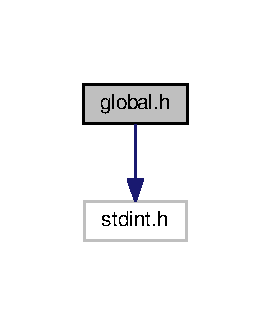
\includegraphics[width=130pt]{global_8h__incl}
\end{center}
\end{figure}
This graph shows which files directly or indirectly include this file\+:
\nopagebreak
\begin{figure}[H]
\begin{center}
\leavevmode
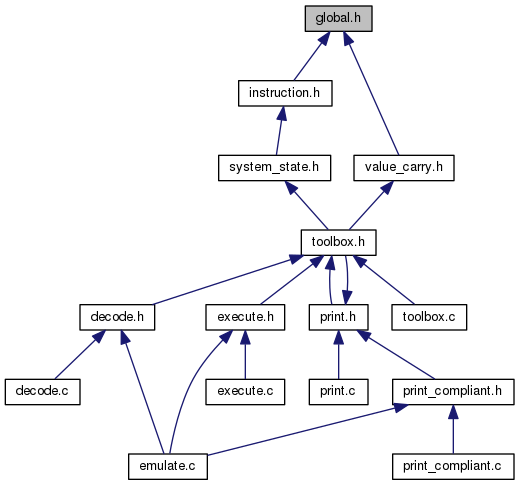
\includegraphics[width=350pt]{global_8h__dep__incl}
\end{center}
\end{figure}
\subsection*{Macros}
\begin{DoxyCompactItemize}
\item 
\#define \hyperlink{global_8h_a5efff3a4a48efbf589e3a2320997d9b9}{N\+U\+M\+\_\+\+R\+E\+G\+I\+S\+T\+E\+RS}~17
\begin{DoxyCompactList}\small\item\em The total number of registers. \end{DoxyCompactList}\item 
\#define \hyperlink{global_8h_ad1d337f69c5203493cb37cb203c33e24}{N\+U\+M\+\_\+\+A\+D\+D\+R\+E\+S\+S\+ES}~65536
\begin{DoxyCompactList}\small\item\em The total number of memory addresses. \end{DoxyCompactList}\item 
\#define \hyperlink{global_8h_a92ed8507d1cd2331ad09275c5c4c1c89}{W\+O\+R\+D\+\_\+\+S\+I\+ZE}~32
\begin{DoxyCompactList}\small\item\em The architecture word size. \end{DoxyCompactList}\item 
\#define \hyperlink{global_8h_a600721f0222b857dc8a3ae59e5077347}{PC}~15
\begin{DoxyCompactList}\small\item\em The register number of the program counter. \end{DoxyCompactList}\item 
\#define \hyperlink{global_8h_a42fdae6e97b3f90e2af0ef1baee0e1ca}{C\+P\+SR}~16
\begin{DoxyCompactList}\small\item\em The register number of the current program status register. \end{DoxyCompactList}\item 
\#define \hyperlink{global_8h_ae35d143ccbd08a6f59f162b3ce9a3141}{M\+A\+S\+K\+\_\+\+F\+I\+R\+S\+T\+\_\+4}~0x\+F\+F\+F\+F\+F\+FF
\begin{DoxyCompactList}\small\item\em A mask which removes the first 4 bits when used with bitwise and. \end{DoxyCompactList}\item 
\#define \hyperlink{global_8h_a76bef05f522db7a5ee54dac38d419fb4}{M\+A\+S\+K\+\_\+\+F\+I\+R\+S\+T\+\_\+6}~0x3\+F\+F\+F\+F\+FF
\begin{DoxyCompactList}\small\item\em A mask which removes the first 6 bits when used with bitwise and. \end{DoxyCompactList}\item 
\#define \hyperlink{global_8h_a87629b54aa0d4536f565c1eacbe73c1b}{M\+A\+S\+K\+\_\+\+F\+I\+R\+S\+T\+\_\+8}~0x\+F\+F\+F\+F\+FF
\begin{DoxyCompactList}\small\item\em A mask which removes the first 8 bits when used with bitwise and. \end{DoxyCompactList}\item 
\#define \hyperlink{global_8h_a8e81dc631606df43e027513e611108ca}{G\+P\+I\+O\+\_\+\+A\+C\+C\+E\+S\+S\+\_\+\+S\+T\+A\+RT}~0x20200000
\begin{DoxyCompactList}\small\item\em The first memory address for accessing G\+P\+IO pins. \end{DoxyCompactList}\item 
\#define \hyperlink{global_8h_a4f31ddcce45b70a39a972d32f4d3214f}{G\+P\+I\+O\+\_\+\+A\+C\+C\+E\+S\+S\+\_\+\+S\+I\+ZE}~12
\begin{DoxyCompactList}\small\item\em The number of bytes allocated for accessing G\+P\+IO pins. \end{DoxyCompactList}\item 
\#define \hyperlink{global_8h_aafecad3506413bdea88cf4203e575121}{G\+P\+I\+O\+\_\+\+C\+L\+E\+A\+R\+\_\+\+S\+T\+A\+RT}~0x20200028
\begin{DoxyCompactList}\small\item\em The first memory address for clearing G\+P\+IO pins. \end{DoxyCompactList}\item 
\#define \hyperlink{global_8h_a663071c046d4ab6fd8fd0cb68f1834d9}{G\+P\+I\+O\+\_\+\+C\+L\+E\+A\+R\+\_\+\+S\+I\+ZE}~4
\begin{DoxyCompactList}\small\item\em The number of bytes allocated for clearing G\+P\+IO pins. \end{DoxyCompactList}\item 
\#define \hyperlink{global_8h_a453005beda34a89be984293ecfc31f84}{G\+P\+I\+O\+\_\+\+S\+E\+T\+\_\+\+S\+T\+A\+RT}~0x2020001C
\begin{DoxyCompactList}\small\item\em The first memory address for setting G\+P\+IO pins. \end{DoxyCompactList}\item 
\#define \hyperlink{global_8h_ac6cd7746692ddb8dfd5dd611950f046c}{G\+P\+I\+O\+\_\+\+S\+E\+T\+\_\+\+S\+I\+ZE}~4
\begin{DoxyCompactList}\small\item\em The number of bytes allocated for setting G\+P\+IO pins. \end{DoxyCompactList}\item 
\#define \hyperlink{global_8h_ae8dd6ba4eeb558fa0dda9626d038dd6d}{C\+O\+M\+P\+L\+I\+A\+N\+T\+\_\+\+M\+O\+DE}~true
\begin{DoxyCompactList}\small\item\em A setting which determines the format of output. \end{DoxyCompactList}\end{DoxyCompactItemize}
\subsection*{Typedefs}
\begin{DoxyCompactItemize}
\item 
typedef uint8\+\_\+t \hyperlink{global_8h_a0661d7d1353e0bca70c64563f635b034}{byte\+\_\+t}
\begin{DoxyCompactList}\small\item\em A type alias for a byte (8 bits). \end{DoxyCompactList}\item 
typedef int8\+\_\+t \hyperlink{global_8h_a462493a8f034b6ade38b69c49a39f52a}{reg\+\_\+address\+\_\+t}
\begin{DoxyCompactList}\small\item\em A type alias for a register number (supports up to 2$^\wedge$8 registers). \end{DoxyCompactList}\item 
typedef uint16\+\_\+t \hyperlink{global_8h_a8f4b132f56a25431714862229639be12}{address\+\_\+t}
\begin{DoxyCompactList}\small\item\em A type alias for a memory address (supports up to 2$^\wedge$16 addresses). \end{DoxyCompactList}\item 
typedef uint32\+\_\+t \hyperlink{global_8h_a0e7744482eed560726581dae7d3cb8b2}{word\+\_\+t}
\begin{DoxyCompactList}\small\item\em A type alias for a word (32 bits). \end{DoxyCompactList}\end{DoxyCompactItemize}
\subsection*{Enumerations}
\begin{DoxyCompactItemize}
\item 
enum \hyperlink{global_8h_a57ba194eedfb8000c1a101fd42abdcf2}{condition\+\_\+t} \{ \\*
\hyperlink{global_8h_a57ba194eedfb8000c1a101fd42abdcf2a9efdc855f3c1477957fb50affec07f8f}{EQ} = 0, 
\hyperlink{global_8h_a57ba194eedfb8000c1a101fd42abdcf2a4d3f872f5054b256b01ee4f2c8cf51db}{NE} = 1, 
\hyperlink{global_8h_a57ba194eedfb8000c1a101fd42abdcf2a558711b4a2a25070b970d85f5926d5ce}{GE} = 0xA, 
\hyperlink{global_8h_a57ba194eedfb8000c1a101fd42abdcf2a486aa221ceeeac475326e85d3d37f571}{LT} = 0xB, 
\\*
\hyperlink{global_8h_a57ba194eedfb8000c1a101fd42abdcf2a12f5476fa04803e6cc72f2198730d892}{GT} = 0xC, 
\hyperlink{global_8h_a57ba194eedfb8000c1a101fd42abdcf2a662ed4b51721a45f07d645d4ca099a61}{LE} = 0xD, 
\hyperlink{global_8h_a57ba194eedfb8000c1a101fd42abdcf2aa0e75d0447532591740f69308c1e7fcf}{AL} = 0xE
 \}\begin{DoxyCompactList}\small\item\em An enum that identifies the type of condition. \end{DoxyCompactList}
\item 
enum \hyperlink{global_8h_aaba7165f28fb81b63cf5b0f1f9dcb40c}{instruction\+\_\+type\+\_\+t} \{ \\*
\hyperlink{global_8h_aaba7165f28fb81b63cf5b0f1f9dcb40caa209bacc9f17fad46996fa40b38c45ae}{D\+PI}, 
\hyperlink{global_8h_aaba7165f28fb81b63cf5b0f1f9dcb40ca086ab1f2f4dac104b6826ebe0eaba8fd}{M\+UL}, 
\hyperlink{global_8h_aaba7165f28fb81b63cf5b0f1f9dcb40ca5aca85f088603150345b57705888081a}{S\+DT}, 
\hyperlink{global_8h_aaba7165f28fb81b63cf5b0f1f9dcb40cab516bd8e9126df5463cbfbdd511e303a}{B\+RA}, 
\\*
\hyperlink{global_8h_aaba7165f28fb81b63cf5b0f1f9dcb40cacb2a8193bc0a747134de34ceb540cdc8}{Z\+ER}, 
\hyperlink{global_8h_aaba7165f28fb81b63cf5b0f1f9dcb40ca4c175fbb65c723226d182dbfd556136a}{N\+UL}
 \}\begin{DoxyCompactList}\small\item\em An enum that identifies the format of the instruction. \end{DoxyCompactList}
\item 
enum \hyperlink{global_8h_a22746cb89e8b2ed0a61876e36446f37f}{shift\+\_\+t} \{ \hyperlink{global_8h_a22746cb89e8b2ed0a61876e36446f37fa0226b11632995cf028f321326046753e}{L\+SL} = 0, 
\hyperlink{global_8h_a22746cb89e8b2ed0a61876e36446f37fa298da67ff8599a09829a91ad0ad3069b}{L\+SR} = 1, 
\hyperlink{global_8h_a22746cb89e8b2ed0a61876e36446f37faf84b730277d260fd0ff17ce3ec05ed5d}{A\+SR} = 2, 
\hyperlink{global_8h_a22746cb89e8b2ed0a61876e36446f37fa7b369e7350ac1a6585413ed60a0d6e10}{R\+OR} = 3
 \}\begin{DoxyCompactList}\small\item\em An enum used for defining the type of shift for the shifter to use. \end{DoxyCompactList}
\item 
enum \hyperlink{global_8h_a8d0559dcae6e251ff5663e79d5581c7d}{opcode\+\_\+t} \{ \\*
\hyperlink{global_8h_a8d0559dcae6e251ff5663e79d5581c7da865555c9f2e0458a7078486aa1b3254f}{A\+ND} = 0x0, 
\hyperlink{global_8h_a8d0559dcae6e251ff5663e79d5581c7da4730d67b92a52e0e6ef813e8805c1623}{E\+OR} = 0x1, 
\hyperlink{global_8h_a8d0559dcae6e251ff5663e79d5581c7da12b733d4941495e86811fe6ceeeff9da}{S\+UB} = 0x2, 
\hyperlink{global_8h_a8d0559dcae6e251ff5663e79d5581c7da1c03efb20082e397c67e1b95c87af195}{R\+SB} = 0x3, 
\\*
\hyperlink{global_8h_a8d0559dcae6e251ff5663e79d5581c7dacfcf145f2788bf340ff3f3098bc54909}{A\+DD} = 0x4, 
\hyperlink{global_8h_a8d0559dcae6e251ff5663e79d5581c7da8a789f931f4c133b3e7b8491e9a9887c}{T\+ST} = 0x8, 
\hyperlink{global_8h_a8d0559dcae6e251ff5663e79d5581c7dac293a3d3f0e7c00325a674d939016c0e}{T\+EQ} = 0x9, 
\hyperlink{global_8h_a8d0559dcae6e251ff5663e79d5581c7da7fd9a97abde63f8c83a4756769aa899e}{C\+MP} = 0xA, 
\\*
\hyperlink{global_8h_a8d0559dcae6e251ff5663e79d5581c7da51e6b781fcc0468896f60da150026bd5}{O\+RR} = 0xC, 
\hyperlink{global_8h_a8d0559dcae6e251ff5663e79d5581c7daa1535ce8fd6caf08009dcae925741d9b}{M\+OV} = 0xD
 \}\begin{DoxyCompactList}\small\item\em An enum used for defining the opcode. \end{DoxyCompactList}
\item 
enum \hyperlink{global_8h_a45ed788e3e7382703f62e6c5a7b528bd}{cpsr\+\_\+flags\+\_\+t} \{ \hyperlink{global_8h_a45ed788e3e7382703f62e6c5a7b528bda2c63acbe79d9f41ba6bb7766e9c37702}{N} = 0x8, 
\hyperlink{global_8h_a45ed788e3e7382703f62e6c5a7b528bdaa70478ce277ffc322f8e1e3418e07355}{Z} = 0x4, 
\hyperlink{global_8h_a45ed788e3e7382703f62e6c5a7b528bda739ce3f516592d245d16fd8a3893472c}{C} = 0x2, 
\hyperlink{global_8h_a45ed788e3e7382703f62e6c5a7b528bda28f41f1144eee94834387e9a6a088bc1}{V} = 0x1
 \}\begin{DoxyCompactList}\small\item\em An enum used for retrieving individual flag bits from C\+P\+SR register. \end{DoxyCompactList}
\end{DoxyCompactItemize}


\subsection{Detailed Description}
Definition of useful constants and type aliases. 



\subsection{Macro Definition Documentation}
\index{global.\+h@{global.\+h}!C\+O\+M\+P\+L\+I\+A\+N\+T\+\_\+\+M\+O\+DE@{C\+O\+M\+P\+L\+I\+A\+N\+T\+\_\+\+M\+O\+DE}}
\index{C\+O\+M\+P\+L\+I\+A\+N\+T\+\_\+\+M\+O\+DE@{C\+O\+M\+P\+L\+I\+A\+N\+T\+\_\+\+M\+O\+DE}!global.\+h@{global.\+h}}
\subsubsection[{\texorpdfstring{C\+O\+M\+P\+L\+I\+A\+N\+T\+\_\+\+M\+O\+DE}{COMPLIANT_MODE}}]{\setlength{\rightskip}{0pt plus 5cm}\#define C\+O\+M\+P\+L\+I\+A\+N\+T\+\_\+\+M\+O\+DE~true}\hypertarget{global_8h_ae8dd6ba4eeb558fa0dda9626d038dd6d}{}\label{global_8h_ae8dd6ba4eeb558fa0dda9626d038dd6d}


A setting which determines the format of output. 


\begin{DoxyItemize}
\item Using C\+O\+M\+P\+L\+I\+A\+N\+T\+\_\+\+M\+O\+DE will print to stdout in the exact format required by test cases. Only registers and memory are printed. Errors are printed to stdout.
\item Otherwise, a much more detailed ouput will be printed, including details on instructions. Formatting is improved. Errors are printed to stderr. The recommended setting is false. 
\end{DoxyItemize}\index{global.\+h@{global.\+h}!C\+P\+SR@{C\+P\+SR}}
\index{C\+P\+SR@{C\+P\+SR}!global.\+h@{global.\+h}}
\subsubsection[{\texorpdfstring{C\+P\+SR}{CPSR}}]{\setlength{\rightskip}{0pt plus 5cm}\#define C\+P\+SR~16}\hypertarget{global_8h_a42fdae6e97b3f90e2af0ef1baee0e1ca}{}\label{global_8h_a42fdae6e97b3f90e2af0ef1baee0e1ca}


The register number of the current program status register. 

\index{global.\+h@{global.\+h}!G\+P\+I\+O\+\_\+\+A\+C\+C\+E\+S\+S\+\_\+\+S\+I\+ZE@{G\+P\+I\+O\+\_\+\+A\+C\+C\+E\+S\+S\+\_\+\+S\+I\+ZE}}
\index{G\+P\+I\+O\+\_\+\+A\+C\+C\+E\+S\+S\+\_\+\+S\+I\+ZE@{G\+P\+I\+O\+\_\+\+A\+C\+C\+E\+S\+S\+\_\+\+S\+I\+ZE}!global.\+h@{global.\+h}}
\subsubsection[{\texorpdfstring{G\+P\+I\+O\+\_\+\+A\+C\+C\+E\+S\+S\+\_\+\+S\+I\+ZE}{GPIO_ACCESS_SIZE}}]{\setlength{\rightskip}{0pt plus 5cm}\#define G\+P\+I\+O\+\_\+\+A\+C\+C\+E\+S\+S\+\_\+\+S\+I\+ZE~12}\hypertarget{global_8h_a4f31ddcce45b70a39a972d32f4d3214f}{}\label{global_8h_a4f31ddcce45b70a39a972d32f4d3214f}


The number of bytes allocated for accessing G\+P\+IO pins. 

\index{global.\+h@{global.\+h}!G\+P\+I\+O\+\_\+\+A\+C\+C\+E\+S\+S\+\_\+\+S\+T\+A\+RT@{G\+P\+I\+O\+\_\+\+A\+C\+C\+E\+S\+S\+\_\+\+S\+T\+A\+RT}}
\index{G\+P\+I\+O\+\_\+\+A\+C\+C\+E\+S\+S\+\_\+\+S\+T\+A\+RT@{G\+P\+I\+O\+\_\+\+A\+C\+C\+E\+S\+S\+\_\+\+S\+T\+A\+RT}!global.\+h@{global.\+h}}
\subsubsection[{\texorpdfstring{G\+P\+I\+O\+\_\+\+A\+C\+C\+E\+S\+S\+\_\+\+S\+T\+A\+RT}{GPIO_ACCESS_START}}]{\setlength{\rightskip}{0pt plus 5cm}\#define G\+P\+I\+O\+\_\+\+A\+C\+C\+E\+S\+S\+\_\+\+S\+T\+A\+RT~0x20200000}\hypertarget{global_8h_a8e81dc631606df43e027513e611108ca}{}\label{global_8h_a8e81dc631606df43e027513e611108ca}


The first memory address for accessing G\+P\+IO pins. 

\index{global.\+h@{global.\+h}!G\+P\+I\+O\+\_\+\+C\+L\+E\+A\+R\+\_\+\+S\+I\+ZE@{G\+P\+I\+O\+\_\+\+C\+L\+E\+A\+R\+\_\+\+S\+I\+ZE}}
\index{G\+P\+I\+O\+\_\+\+C\+L\+E\+A\+R\+\_\+\+S\+I\+ZE@{G\+P\+I\+O\+\_\+\+C\+L\+E\+A\+R\+\_\+\+S\+I\+ZE}!global.\+h@{global.\+h}}
\subsubsection[{\texorpdfstring{G\+P\+I\+O\+\_\+\+C\+L\+E\+A\+R\+\_\+\+S\+I\+ZE}{GPIO_CLEAR_SIZE}}]{\setlength{\rightskip}{0pt plus 5cm}\#define G\+P\+I\+O\+\_\+\+C\+L\+E\+A\+R\+\_\+\+S\+I\+ZE~4}\hypertarget{global_8h_a663071c046d4ab6fd8fd0cb68f1834d9}{}\label{global_8h_a663071c046d4ab6fd8fd0cb68f1834d9}


The number of bytes allocated for clearing G\+P\+IO pins. 

\index{global.\+h@{global.\+h}!G\+P\+I\+O\+\_\+\+C\+L\+E\+A\+R\+\_\+\+S\+T\+A\+RT@{G\+P\+I\+O\+\_\+\+C\+L\+E\+A\+R\+\_\+\+S\+T\+A\+RT}}
\index{G\+P\+I\+O\+\_\+\+C\+L\+E\+A\+R\+\_\+\+S\+T\+A\+RT@{G\+P\+I\+O\+\_\+\+C\+L\+E\+A\+R\+\_\+\+S\+T\+A\+RT}!global.\+h@{global.\+h}}
\subsubsection[{\texorpdfstring{G\+P\+I\+O\+\_\+\+C\+L\+E\+A\+R\+\_\+\+S\+T\+A\+RT}{GPIO_CLEAR_START}}]{\setlength{\rightskip}{0pt plus 5cm}\#define G\+P\+I\+O\+\_\+\+C\+L\+E\+A\+R\+\_\+\+S\+T\+A\+RT~0x20200028}\hypertarget{global_8h_aafecad3506413bdea88cf4203e575121}{}\label{global_8h_aafecad3506413bdea88cf4203e575121}


The first memory address for clearing G\+P\+IO pins. 

\index{global.\+h@{global.\+h}!G\+P\+I\+O\+\_\+\+S\+E\+T\+\_\+\+S\+I\+ZE@{G\+P\+I\+O\+\_\+\+S\+E\+T\+\_\+\+S\+I\+ZE}}
\index{G\+P\+I\+O\+\_\+\+S\+E\+T\+\_\+\+S\+I\+ZE@{G\+P\+I\+O\+\_\+\+S\+E\+T\+\_\+\+S\+I\+ZE}!global.\+h@{global.\+h}}
\subsubsection[{\texorpdfstring{G\+P\+I\+O\+\_\+\+S\+E\+T\+\_\+\+S\+I\+ZE}{GPIO_SET_SIZE}}]{\setlength{\rightskip}{0pt plus 5cm}\#define G\+P\+I\+O\+\_\+\+S\+E\+T\+\_\+\+S\+I\+ZE~4}\hypertarget{global_8h_ac6cd7746692ddb8dfd5dd611950f046c}{}\label{global_8h_ac6cd7746692ddb8dfd5dd611950f046c}


The number of bytes allocated for setting G\+P\+IO pins. 

\index{global.\+h@{global.\+h}!G\+P\+I\+O\+\_\+\+S\+E\+T\+\_\+\+S\+T\+A\+RT@{G\+P\+I\+O\+\_\+\+S\+E\+T\+\_\+\+S\+T\+A\+RT}}
\index{G\+P\+I\+O\+\_\+\+S\+E\+T\+\_\+\+S\+T\+A\+RT@{G\+P\+I\+O\+\_\+\+S\+E\+T\+\_\+\+S\+T\+A\+RT}!global.\+h@{global.\+h}}
\subsubsection[{\texorpdfstring{G\+P\+I\+O\+\_\+\+S\+E\+T\+\_\+\+S\+T\+A\+RT}{GPIO_SET_START}}]{\setlength{\rightskip}{0pt plus 5cm}\#define G\+P\+I\+O\+\_\+\+S\+E\+T\+\_\+\+S\+T\+A\+RT~0x2020001C}\hypertarget{global_8h_a453005beda34a89be984293ecfc31f84}{}\label{global_8h_a453005beda34a89be984293ecfc31f84}


The first memory address for setting G\+P\+IO pins. 

\index{global.\+h@{global.\+h}!M\+A\+S\+K\+\_\+\+F\+I\+R\+S\+T\+\_\+4@{M\+A\+S\+K\+\_\+\+F\+I\+R\+S\+T\+\_\+4}}
\index{M\+A\+S\+K\+\_\+\+F\+I\+R\+S\+T\+\_\+4@{M\+A\+S\+K\+\_\+\+F\+I\+R\+S\+T\+\_\+4}!global.\+h@{global.\+h}}
\subsubsection[{\texorpdfstring{M\+A\+S\+K\+\_\+\+F\+I\+R\+S\+T\+\_\+4}{MASK_FIRST_4}}]{\setlength{\rightskip}{0pt plus 5cm}\#define M\+A\+S\+K\+\_\+\+F\+I\+R\+S\+T\+\_\+4~0x\+F\+F\+F\+F\+F\+FF}\hypertarget{global_8h_ae35d143ccbd08a6f59f162b3ce9a3141}{}\label{global_8h_ae35d143ccbd08a6f59f162b3ce9a3141}


A mask which removes the first 4 bits when used with bitwise and. 

\index{global.\+h@{global.\+h}!M\+A\+S\+K\+\_\+\+F\+I\+R\+S\+T\+\_\+6@{M\+A\+S\+K\+\_\+\+F\+I\+R\+S\+T\+\_\+6}}
\index{M\+A\+S\+K\+\_\+\+F\+I\+R\+S\+T\+\_\+6@{M\+A\+S\+K\+\_\+\+F\+I\+R\+S\+T\+\_\+6}!global.\+h@{global.\+h}}
\subsubsection[{\texorpdfstring{M\+A\+S\+K\+\_\+\+F\+I\+R\+S\+T\+\_\+6}{MASK_FIRST_6}}]{\setlength{\rightskip}{0pt plus 5cm}\#define M\+A\+S\+K\+\_\+\+F\+I\+R\+S\+T\+\_\+6~0x3\+F\+F\+F\+F\+FF}\hypertarget{global_8h_a76bef05f522db7a5ee54dac38d419fb4}{}\label{global_8h_a76bef05f522db7a5ee54dac38d419fb4}


A mask which removes the first 6 bits when used with bitwise and. 

\index{global.\+h@{global.\+h}!M\+A\+S\+K\+\_\+\+F\+I\+R\+S\+T\+\_\+8@{M\+A\+S\+K\+\_\+\+F\+I\+R\+S\+T\+\_\+8}}
\index{M\+A\+S\+K\+\_\+\+F\+I\+R\+S\+T\+\_\+8@{M\+A\+S\+K\+\_\+\+F\+I\+R\+S\+T\+\_\+8}!global.\+h@{global.\+h}}
\subsubsection[{\texorpdfstring{M\+A\+S\+K\+\_\+\+F\+I\+R\+S\+T\+\_\+8}{MASK_FIRST_8}}]{\setlength{\rightskip}{0pt plus 5cm}\#define M\+A\+S\+K\+\_\+\+F\+I\+R\+S\+T\+\_\+8~0x\+F\+F\+F\+F\+FF}\hypertarget{global_8h_a87629b54aa0d4536f565c1eacbe73c1b}{}\label{global_8h_a87629b54aa0d4536f565c1eacbe73c1b}


A mask which removes the first 8 bits when used with bitwise and. 

\index{global.\+h@{global.\+h}!N\+U\+M\+\_\+\+A\+D\+D\+R\+E\+S\+S\+ES@{N\+U\+M\+\_\+\+A\+D\+D\+R\+E\+S\+S\+ES}}
\index{N\+U\+M\+\_\+\+A\+D\+D\+R\+E\+S\+S\+ES@{N\+U\+M\+\_\+\+A\+D\+D\+R\+E\+S\+S\+ES}!global.\+h@{global.\+h}}
\subsubsection[{\texorpdfstring{N\+U\+M\+\_\+\+A\+D\+D\+R\+E\+S\+S\+ES}{NUM_ADDRESSES}}]{\setlength{\rightskip}{0pt plus 5cm}\#define N\+U\+M\+\_\+\+A\+D\+D\+R\+E\+S\+S\+ES~65536}\hypertarget{global_8h_ad1d337f69c5203493cb37cb203c33e24}{}\label{global_8h_ad1d337f69c5203493cb37cb203c33e24}


The total number of memory addresses. 

\index{global.\+h@{global.\+h}!N\+U\+M\+\_\+\+R\+E\+G\+I\+S\+T\+E\+RS@{N\+U\+M\+\_\+\+R\+E\+G\+I\+S\+T\+E\+RS}}
\index{N\+U\+M\+\_\+\+R\+E\+G\+I\+S\+T\+E\+RS@{N\+U\+M\+\_\+\+R\+E\+G\+I\+S\+T\+E\+RS}!global.\+h@{global.\+h}}
\subsubsection[{\texorpdfstring{N\+U\+M\+\_\+\+R\+E\+G\+I\+S\+T\+E\+RS}{NUM_REGISTERS}}]{\setlength{\rightskip}{0pt plus 5cm}\#define N\+U\+M\+\_\+\+R\+E\+G\+I\+S\+T\+E\+RS~17}\hypertarget{global_8h_a5efff3a4a48efbf589e3a2320997d9b9}{}\label{global_8h_a5efff3a4a48efbf589e3a2320997d9b9}


The total number of registers. 

\index{global.\+h@{global.\+h}!PC@{PC}}
\index{PC@{PC}!global.\+h@{global.\+h}}
\subsubsection[{\texorpdfstring{PC}{PC}}]{\setlength{\rightskip}{0pt plus 5cm}\#define PC~15}\hypertarget{global_8h_a600721f0222b857dc8a3ae59e5077347}{}\label{global_8h_a600721f0222b857dc8a3ae59e5077347}


The register number of the program counter. 

\index{global.\+h@{global.\+h}!W\+O\+R\+D\+\_\+\+S\+I\+ZE@{W\+O\+R\+D\+\_\+\+S\+I\+ZE}}
\index{W\+O\+R\+D\+\_\+\+S\+I\+ZE@{W\+O\+R\+D\+\_\+\+S\+I\+ZE}!global.\+h@{global.\+h}}
\subsubsection[{\texorpdfstring{W\+O\+R\+D\+\_\+\+S\+I\+ZE}{WORD_SIZE}}]{\setlength{\rightskip}{0pt plus 5cm}\#define W\+O\+R\+D\+\_\+\+S\+I\+ZE~32}\hypertarget{global_8h_a92ed8507d1cd2331ad09275c5c4c1c89}{}\label{global_8h_a92ed8507d1cd2331ad09275c5c4c1c89}


The architecture word size. 



\subsection{Typedef Documentation}
\index{global.\+h@{global.\+h}!address\+\_\+t@{address\+\_\+t}}
\index{address\+\_\+t@{address\+\_\+t}!global.\+h@{global.\+h}}
\subsubsection[{\texorpdfstring{address\+\_\+t}{address_t}}]{\setlength{\rightskip}{0pt plus 5cm}typedef uint16\+\_\+t {\bf address\+\_\+t}}\hypertarget{global_8h_a8f4b132f56a25431714862229639be12}{}\label{global_8h_a8f4b132f56a25431714862229639be12}


A type alias for a memory address (supports up to 2$^\wedge$16 addresses). 

\index{global.\+h@{global.\+h}!byte\+\_\+t@{byte\+\_\+t}}
\index{byte\+\_\+t@{byte\+\_\+t}!global.\+h@{global.\+h}}
\subsubsection[{\texorpdfstring{byte\+\_\+t}{byte_t}}]{\setlength{\rightskip}{0pt plus 5cm}typedef uint8\+\_\+t {\bf byte\+\_\+t}}\hypertarget{global_8h_a0661d7d1353e0bca70c64563f635b034}{}\label{global_8h_a0661d7d1353e0bca70c64563f635b034}


A type alias for a byte (8 bits). 

\index{global.\+h@{global.\+h}!reg\+\_\+address\+\_\+t@{reg\+\_\+address\+\_\+t}}
\index{reg\+\_\+address\+\_\+t@{reg\+\_\+address\+\_\+t}!global.\+h@{global.\+h}}
\subsubsection[{\texorpdfstring{reg\+\_\+address\+\_\+t}{reg_address_t}}]{\setlength{\rightskip}{0pt plus 5cm}typedef int8\+\_\+t {\bf reg\+\_\+address\+\_\+t}}\hypertarget{global_8h_a462493a8f034b6ade38b69c49a39f52a}{}\label{global_8h_a462493a8f034b6ade38b69c49a39f52a}


A type alias for a register number (supports up to 2$^\wedge$8 registers). 

\index{global.\+h@{global.\+h}!word\+\_\+t@{word\+\_\+t}}
\index{word\+\_\+t@{word\+\_\+t}!global.\+h@{global.\+h}}
\subsubsection[{\texorpdfstring{word\+\_\+t}{word_t}}]{\setlength{\rightskip}{0pt plus 5cm}typedef uint32\+\_\+t {\bf word\+\_\+t}}\hypertarget{global_8h_a0e7744482eed560726581dae7d3cb8b2}{}\label{global_8h_a0e7744482eed560726581dae7d3cb8b2}


A type alias for a word (32 bits). 



\subsection{Enumeration Type Documentation}
\index{global.\+h@{global.\+h}!condition\+\_\+t@{condition\+\_\+t}}
\index{condition\+\_\+t@{condition\+\_\+t}!global.\+h@{global.\+h}}
\subsubsection[{\texorpdfstring{condition\+\_\+t}{condition_t}}]{\setlength{\rightskip}{0pt plus 5cm}enum {\bf condition\+\_\+t}}\hypertarget{global_8h_a57ba194eedfb8000c1a101fd42abdcf2}{}\label{global_8h_a57ba194eedfb8000c1a101fd42abdcf2}


An enum that identifies the type of condition. 

\begin{Desc}
\item[Enumerator]\par
\begin{description}
\index{EQ@{EQ}!global.\+h@{global.\+h}}\index{global.\+h@{global.\+h}!EQ@{EQ}}\item[{\em 
EQ\hypertarget{global_8h_a57ba194eedfb8000c1a101fd42abdcf2a9efdc855f3c1477957fb50affec07f8f}{}\label{global_8h_a57ba194eedfb8000c1a101fd42abdcf2a9efdc855f3c1477957fb50affec07f8f}
}]Equal. \index{NE@{NE}!global.\+h@{global.\+h}}\index{global.\+h@{global.\+h}!NE@{NE}}\item[{\em 
NE\hypertarget{global_8h_a57ba194eedfb8000c1a101fd42abdcf2a4d3f872f5054b256b01ee4f2c8cf51db}{}\label{global_8h_a57ba194eedfb8000c1a101fd42abdcf2a4d3f872f5054b256b01ee4f2c8cf51db}
}]Not equal. \index{GE@{GE}!global.\+h@{global.\+h}}\index{global.\+h@{global.\+h}!GE@{GE}}\item[{\em 
GE\hypertarget{global_8h_a57ba194eedfb8000c1a101fd42abdcf2a558711b4a2a25070b970d85f5926d5ce}{}\label{global_8h_a57ba194eedfb8000c1a101fd42abdcf2a558711b4a2a25070b970d85f5926d5ce}
}]Greater or equal. \index{LT@{LT}!global.\+h@{global.\+h}}\index{global.\+h@{global.\+h}!LT@{LT}}\item[{\em 
LT\hypertarget{global_8h_a57ba194eedfb8000c1a101fd42abdcf2a486aa221ceeeac475326e85d3d37f571}{}\label{global_8h_a57ba194eedfb8000c1a101fd42abdcf2a486aa221ceeeac475326e85d3d37f571}
}]Less than. \index{GT@{GT}!global.\+h@{global.\+h}}\index{global.\+h@{global.\+h}!GT@{GT}}\item[{\em 
GT\hypertarget{global_8h_a57ba194eedfb8000c1a101fd42abdcf2a12f5476fa04803e6cc72f2198730d892}{}\label{global_8h_a57ba194eedfb8000c1a101fd42abdcf2a12f5476fa04803e6cc72f2198730d892}
}]Greater than. \index{LE@{LE}!global.\+h@{global.\+h}}\index{global.\+h@{global.\+h}!LE@{LE}}\item[{\em 
LE\hypertarget{global_8h_a57ba194eedfb8000c1a101fd42abdcf2a662ed4b51721a45f07d645d4ca099a61}{}\label{global_8h_a57ba194eedfb8000c1a101fd42abdcf2a662ed4b51721a45f07d645d4ca099a61}
}]Less than or equal to. \index{AL@{AL}!global.\+h@{global.\+h}}\index{global.\+h@{global.\+h}!AL@{AL}}\item[{\em 
AL\hypertarget{global_8h_a57ba194eedfb8000c1a101fd42abdcf2aa0e75d0447532591740f69308c1e7fcf}{}\label{global_8h_a57ba194eedfb8000c1a101fd42abdcf2aa0e75d0447532591740f69308c1e7fcf}
}]No condition (always). \end{description}
\end{Desc}
\index{global.\+h@{global.\+h}!cpsr\+\_\+flags\+\_\+t@{cpsr\+\_\+flags\+\_\+t}}
\index{cpsr\+\_\+flags\+\_\+t@{cpsr\+\_\+flags\+\_\+t}!global.\+h@{global.\+h}}
\subsubsection[{\texorpdfstring{cpsr\+\_\+flags\+\_\+t}{cpsr_flags_t}}]{\setlength{\rightskip}{0pt plus 5cm}enum {\bf cpsr\+\_\+flags\+\_\+t}}\hypertarget{global_8h_a45ed788e3e7382703f62e6c5a7b528bd}{}\label{global_8h_a45ed788e3e7382703f62e6c5a7b528bd}


An enum used for retrieving individual flag bits from C\+P\+SR register. 

\begin{Desc}
\item[Enumerator]\par
\begin{description}
\index{N@{N}!global.\+h@{global.\+h}}\index{global.\+h@{global.\+h}!N@{N}}\item[{\em 
N\hypertarget{global_8h_a45ed788e3e7382703f62e6c5a7b528bda2c63acbe79d9f41ba6bb7766e9c37702}{}\label{global_8h_a45ed788e3e7382703f62e6c5a7b528bda2c63acbe79d9f41ba6bb7766e9c37702}
}]N (bit 4)\+: the last result was negative. \index{Z@{Z}!global.\+h@{global.\+h}}\index{global.\+h@{global.\+h}!Z@{Z}}\item[{\em 
Z\hypertarget{global_8h_a45ed788e3e7382703f62e6c5a7b528bdaa70478ce277ffc322f8e1e3418e07355}{}\label{global_8h_a45ed788e3e7382703f62e6c5a7b528bdaa70478ce277ffc322f8e1e3418e07355}
}]Z (bit 3)\+: the last result was zero. \index{C@{C}!global.\+h@{global.\+h}}\index{global.\+h@{global.\+h}!C@{C}}\item[{\em 
C\hypertarget{global_8h_a45ed788e3e7382703f62e6c5a7b528bda739ce3f516592d245d16fd8a3893472c}{}\label{global_8h_a45ed788e3e7382703f62e6c5a7b528bda739ce3f516592d245d16fd8a3893472c}
}]C (bit 2)\+: the last result caused a bit to be carried out. \index{V@{V}!global.\+h@{global.\+h}}\index{global.\+h@{global.\+h}!V@{V}}\item[{\em 
V\hypertarget{global_8h_a45ed788e3e7382703f62e6c5a7b528bda28f41f1144eee94834387e9a6a088bc1}{}\label{global_8h_a45ed788e3e7382703f62e6c5a7b528bda28f41f1144eee94834387e9a6a088bc1}
}]V (bit 1)\+: the last result overflowed. \end{description}
\end{Desc}
\index{global.\+h@{global.\+h}!instruction\+\_\+type\+\_\+t@{instruction\+\_\+type\+\_\+t}}
\index{instruction\+\_\+type\+\_\+t@{instruction\+\_\+type\+\_\+t}!global.\+h@{global.\+h}}
\subsubsection[{\texorpdfstring{instruction\+\_\+type\+\_\+t}{instruction_type_t}}]{\setlength{\rightskip}{0pt plus 5cm}enum {\bf instruction\+\_\+type\+\_\+t}}\hypertarget{global_8h_aaba7165f28fb81b63cf5b0f1f9dcb40c}{}\label{global_8h_aaba7165f28fb81b63cf5b0f1f9dcb40c}


An enum that identifies the format of the instruction. 

\begin{Desc}
\item[Enumerator]\par
\begin{description}
\index{D\+PI@{D\+PI}!global.\+h@{global.\+h}}\index{global.\+h@{global.\+h}!D\+PI@{D\+PI}}\item[{\em 
D\+PI\hypertarget{global_8h_aaba7165f28fb81b63cf5b0f1f9dcb40caa209bacc9f17fad46996fa40b38c45ae}{}\label{global_8h_aaba7165f28fb81b63cf5b0f1f9dcb40caa209bacc9f17fad46996fa40b38c45ae}
}]Data processing instruction. \index{M\+UL@{M\+UL}!global.\+h@{global.\+h}}\index{global.\+h@{global.\+h}!M\+UL@{M\+UL}}\item[{\em 
M\+UL\hypertarget{global_8h_aaba7165f28fb81b63cf5b0f1f9dcb40ca086ab1f2f4dac104b6826ebe0eaba8fd}{}\label{global_8h_aaba7165f28fb81b63cf5b0f1f9dcb40ca086ab1f2f4dac104b6826ebe0eaba8fd}
}]Multiply instruction. \index{S\+DT@{S\+DT}!global.\+h@{global.\+h}}\index{global.\+h@{global.\+h}!S\+DT@{S\+DT}}\item[{\em 
S\+DT\hypertarget{global_8h_aaba7165f28fb81b63cf5b0f1f9dcb40ca5aca85f088603150345b57705888081a}{}\label{global_8h_aaba7165f28fb81b63cf5b0f1f9dcb40ca5aca85f088603150345b57705888081a}
}]Single data transfer instruction. \index{B\+RA@{B\+RA}!global.\+h@{global.\+h}}\index{global.\+h@{global.\+h}!B\+RA@{B\+RA}}\item[{\em 
B\+RA\hypertarget{global_8h_aaba7165f28fb81b63cf5b0f1f9dcb40cab516bd8e9126df5463cbfbdd511e303a}{}\label{global_8h_aaba7165f28fb81b63cf5b0f1f9dcb40cab516bd8e9126df5463cbfbdd511e303a}
}]Branch instruction. \index{Z\+ER@{Z\+ER}!global.\+h@{global.\+h}}\index{global.\+h@{global.\+h}!Z\+ER@{Z\+ER}}\item[{\em 
Z\+ER\hypertarget{global_8h_aaba7165f28fb81b63cf5b0f1f9dcb40cacb2a8193bc0a747134de34ceb540cdc8}{}\label{global_8h_aaba7165f28fb81b63cf5b0f1f9dcb40cacb2a8193bc0a747134de34ceb540cdc8}
}]All zero (S\+T\+OP) instruction. \index{N\+UL@{N\+UL}!global.\+h@{global.\+h}}\index{global.\+h@{global.\+h}!N\+UL@{N\+UL}}\item[{\em 
N\+UL\hypertarget{global_8h_aaba7165f28fb81b63cf5b0f1f9dcb40ca4c175fbb65c723226d182dbfd556136a}{}\label{global_8h_aaba7165f28fb81b63cf5b0f1f9dcb40ca4c175fbb65c723226d182dbfd556136a}
}]N\+U\+LL (not present) instruction. \end{description}
\end{Desc}
\index{global.\+h@{global.\+h}!opcode\+\_\+t@{opcode\+\_\+t}}
\index{opcode\+\_\+t@{opcode\+\_\+t}!global.\+h@{global.\+h}}
\subsubsection[{\texorpdfstring{opcode\+\_\+t}{opcode_t}}]{\setlength{\rightskip}{0pt plus 5cm}enum {\bf opcode\+\_\+t}}\hypertarget{global_8h_a8d0559dcae6e251ff5663e79d5581c7d}{}\label{global_8h_a8d0559dcae6e251ff5663e79d5581c7d}


An enum used for defining the opcode. 

\begin{Desc}
\item[Enumerator]\par
\begin{description}
\index{A\+ND@{A\+ND}!global.\+h@{global.\+h}}\index{global.\+h@{global.\+h}!A\+ND@{A\+ND}}\item[{\em 
A\+ND\hypertarget{global_8h_a8d0559dcae6e251ff5663e79d5581c7da865555c9f2e0458a7078486aa1b3254f}{}\label{global_8h_a8d0559dcae6e251ff5663e79d5581c7da865555c9f2e0458a7078486aa1b3254f}
}]And. \index{E\+OR@{E\+OR}!global.\+h@{global.\+h}}\index{global.\+h@{global.\+h}!E\+OR@{E\+OR}}\item[{\em 
E\+OR\hypertarget{global_8h_a8d0559dcae6e251ff5663e79d5581c7da4730d67b92a52e0e6ef813e8805c1623}{}\label{global_8h_a8d0559dcae6e251ff5663e79d5581c7da4730d67b92a52e0e6ef813e8805c1623}
}]Exclusive or. \index{S\+UB@{S\+UB}!global.\+h@{global.\+h}}\index{global.\+h@{global.\+h}!S\+UB@{S\+UB}}\item[{\em 
S\+UB\hypertarget{global_8h_a8d0559dcae6e251ff5663e79d5581c7da12b733d4941495e86811fe6ceeeff9da}{}\label{global_8h_a8d0559dcae6e251ff5663e79d5581c7da12b733d4941495e86811fe6ceeeff9da}
}]Subtract. \index{R\+SB@{R\+SB}!global.\+h@{global.\+h}}\index{global.\+h@{global.\+h}!R\+SB@{R\+SB}}\item[{\em 
R\+SB\hypertarget{global_8h_a8d0559dcae6e251ff5663e79d5581c7da1c03efb20082e397c67e1b95c87af195}{}\label{global_8h_a8d0559dcae6e251ff5663e79d5581c7da1c03efb20082e397c67e1b95c87af195}
}]Reverse subtract. \index{A\+DD@{A\+DD}!global.\+h@{global.\+h}}\index{global.\+h@{global.\+h}!A\+DD@{A\+DD}}\item[{\em 
A\+DD\hypertarget{global_8h_a8d0559dcae6e251ff5663e79d5581c7dacfcf145f2788bf340ff3f3098bc54909}{}\label{global_8h_a8d0559dcae6e251ff5663e79d5581c7dacfcf145f2788bf340ff3f3098bc54909}
}]Add. \index{T\+ST@{T\+ST}!global.\+h@{global.\+h}}\index{global.\+h@{global.\+h}!T\+ST@{T\+ST}}\item[{\em 
T\+ST\hypertarget{global_8h_a8d0559dcae6e251ff5663e79d5581c7da8a789f931f4c133b3e7b8491e9a9887c}{}\label{global_8h_a8d0559dcae6e251ff5663e79d5581c7da8a789f931f4c133b3e7b8491e9a9887c}
}]And, set flags only. \index{T\+EQ@{T\+EQ}!global.\+h@{global.\+h}}\index{global.\+h@{global.\+h}!T\+EQ@{T\+EQ}}\item[{\em 
T\+EQ\hypertarget{global_8h_a8d0559dcae6e251ff5663e79d5581c7dac293a3d3f0e7c00325a674d939016c0e}{}\label{global_8h_a8d0559dcae6e251ff5663e79d5581c7dac293a3d3f0e7c00325a674d939016c0e}
}]Exclusive or, set flags only. \index{C\+MP@{C\+MP}!global.\+h@{global.\+h}}\index{global.\+h@{global.\+h}!C\+MP@{C\+MP}}\item[{\em 
C\+MP\hypertarget{global_8h_a8d0559dcae6e251ff5663e79d5581c7da7fd9a97abde63f8c83a4756769aa899e}{}\label{global_8h_a8d0559dcae6e251ff5663e79d5581c7da7fd9a97abde63f8c83a4756769aa899e}
}]Subtract, set flags only. \index{O\+RR@{O\+RR}!global.\+h@{global.\+h}}\index{global.\+h@{global.\+h}!O\+RR@{O\+RR}}\item[{\em 
O\+RR\hypertarget{global_8h_a8d0559dcae6e251ff5663e79d5581c7da51e6b781fcc0468896f60da150026bd5}{}\label{global_8h_a8d0559dcae6e251ff5663e79d5581c7da51e6b781fcc0468896f60da150026bd5}
}]Or. \index{M\+OV@{M\+OV}!global.\+h@{global.\+h}}\index{global.\+h@{global.\+h}!M\+OV@{M\+OV}}\item[{\em 
M\+OV\hypertarget{global_8h_a8d0559dcae6e251ff5663e79d5581c7daa1535ce8fd6caf08009dcae925741d9b}{}\label{global_8h_a8d0559dcae6e251ff5663e79d5581c7daa1535ce8fd6caf08009dcae925741d9b}
}]Move. \end{description}
\end{Desc}
\index{global.\+h@{global.\+h}!shift\+\_\+t@{shift\+\_\+t}}
\index{shift\+\_\+t@{shift\+\_\+t}!global.\+h@{global.\+h}}
\subsubsection[{\texorpdfstring{shift\+\_\+t}{shift_t}}]{\setlength{\rightskip}{0pt plus 5cm}enum {\bf shift\+\_\+t}}\hypertarget{global_8h_a22746cb89e8b2ed0a61876e36446f37f}{}\label{global_8h_a22746cb89e8b2ed0a61876e36446f37f}


An enum used for defining the type of shift for the shifter to use. 

\begin{Desc}
\item[Enumerator]\par
\begin{description}
\index{L\+SL@{L\+SL}!global.\+h@{global.\+h}}\index{global.\+h@{global.\+h}!L\+SL@{L\+SL}}\item[{\em 
L\+SL\hypertarget{global_8h_a22746cb89e8b2ed0a61876e36446f37fa0226b11632995cf028f321326046753e}{}\label{global_8h_a22746cb89e8b2ed0a61876e36446f37fa0226b11632995cf028f321326046753e}
}]Logical shift left. \index{L\+SR@{L\+SR}!global.\+h@{global.\+h}}\index{global.\+h@{global.\+h}!L\+SR@{L\+SR}}\item[{\em 
L\+SR\hypertarget{global_8h_a22746cb89e8b2ed0a61876e36446f37fa298da67ff8599a09829a91ad0ad3069b}{}\label{global_8h_a22746cb89e8b2ed0a61876e36446f37fa298da67ff8599a09829a91ad0ad3069b}
}]Logical shift right. \index{A\+SR@{A\+SR}!global.\+h@{global.\+h}}\index{global.\+h@{global.\+h}!A\+SR@{A\+SR}}\item[{\em 
A\+SR\hypertarget{global_8h_a22746cb89e8b2ed0a61876e36446f37faf84b730277d260fd0ff17ce3ec05ed5d}{}\label{global_8h_a22746cb89e8b2ed0a61876e36446f37faf84b730277d260fd0ff17ce3ec05ed5d}
}]Arithmetic shift right. \index{R\+OR@{R\+OR}!global.\+h@{global.\+h}}\index{global.\+h@{global.\+h}!R\+OR@{R\+OR}}\item[{\em 
R\+OR\hypertarget{global_8h_a22746cb89e8b2ed0a61876e36446f37fa7b369e7350ac1a6585413ed60a0d6e10}{}\label{global_8h_a22746cb89e8b2ed0a61876e36446f37fa7b369e7350ac1a6585413ed60a0d6e10}
}]Rotate right. \end{description}
\end{Desc}

\hypertarget{instruction_8h}{}\section{instruction.\+h File Reference}
\label{instruction_8h}\index{instruction.\+h@{instruction.\+h}}


A header to define the \hyperlink{structinstruction__t}{instruction\+\_\+t} type.  


{\ttfamily \#include $<$stdbool.\+h$>$}\\*
{\ttfamily \#include \char`\"{}global.\+h\char`\"{}}\\*
Include dependency graph for instruction.\+h\+:\nopagebreak
\begin{figure}[H]
\begin{center}
\leavevmode
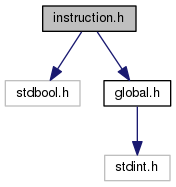
\includegraphics[width=204pt]{instruction_8h__incl}
\end{center}
\end{figure}
This graph shows which files directly or indirectly include this file\+:\nopagebreak
\begin{figure}[H]
\begin{center}
\leavevmode
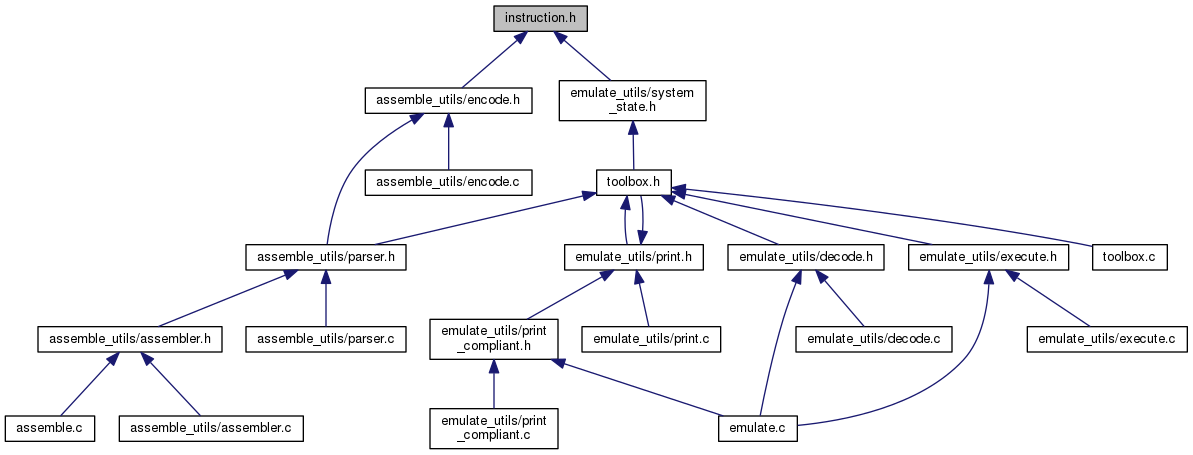
\includegraphics[width=350pt]{instruction_8h__dep__incl}
\end{center}
\end{figure}
\subsection*{Data Structures}
\begin{DoxyCompactItemize}
\item 
struct \hyperlink{structinstruction__t}{instruction\+\_\+t}
\begin{DoxyCompactList}\small\item\em A struct that holds information about a decoded instruction. \end{DoxyCompactList}\end{DoxyCompactItemize}


\subsection{Detailed Description}
A header to define the \hyperlink{structinstruction__t}{instruction\+\_\+t} type. 


\hypertarget{print_8c}{}\section{emulate\+\_\+utils/print.c File Reference}
\label{print_8c}\index{emulate\+\_\+utils/print.\+c@{emulate\+\_\+utils/print.\+c}}


Functions for printing system details to standard output.  


{\ttfamily \#include \char`\"{}print.\+h\char`\"{}}\\*
Include dependency graph for print.\+c\+:\nopagebreak
\begin{figure}[H]
\begin{center}
\leavevmode
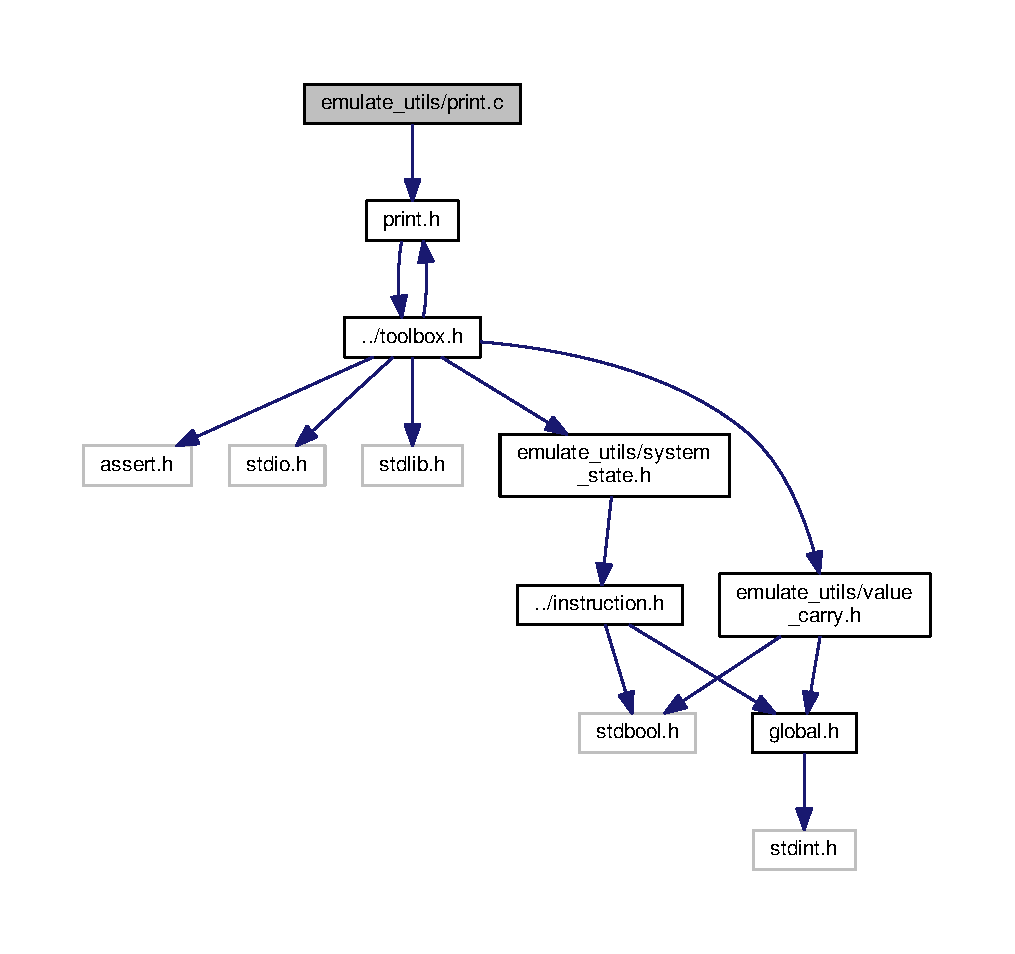
\includegraphics[width=350pt]{print_8c__incl}
\end{center}
\end{figure}
\subsection*{Functions}
\begin{DoxyCompactItemize}
\item 
void \hyperlink{print_8c_aa6201dccc033aad617c0d854e18f0915}{print\+\_\+array} (\hyperlink{global_8h_a0661d7d1353e0bca70c64563f635b034}{byte\+\_\+t} $\ast$memory, size\+\_\+t bytes\+\_\+to\+\_\+print)
\begin{DoxyCompactList}\small\item\em Prints a given number of bytes, from an array of bytes. \end{DoxyCompactList}\item 
void \hyperlink{print_8c_ae3374a188808236ad908ca5300516ae6}{print\+\_\+system\+\_\+state} (\hyperlink{structsystem__state__t}{system\+\_\+state\+\_\+t} $\ast$machine)
\begin{DoxyCompactList}\small\item\em Prints system state details. \end{DoxyCompactList}\item 
void \hyperlink{print_8c_aa0d2fa15c6ec7ec862fb74640427e510}{print\+\_\+registers} (\hyperlink{structsystem__state__t}{system\+\_\+state\+\_\+t} $\ast$machine)
\begin{DoxyCompactList}\small\item\em Prints the values of registers. \end{DoxyCompactList}\item 
void \hyperlink{print_8c_a19bd450ad0dc7d7d873f9add3989c0b5}{print\+\_\+memory} (\hyperlink{structsystem__state__t}{system\+\_\+state\+\_\+t} $\ast$machine)
\begin{DoxyCompactList}\small\item\em Prints any non-\/zero words from memory. \end{DoxyCompactList}\item 
void \hyperlink{print_8c_a48a0096457ff1ab2d250b08778a5c4a2}{print\+\_\+decoded\+\_\+instruction} (\hyperlink{structsystem__state__t}{system\+\_\+state\+\_\+t} $\ast$machine)
\begin{DoxyCompactList}\small\item\em Prints details for the decoded instruction. \end{DoxyCompactList}\item 
void \hyperlink{print_8c_a09f4c8695471e9d40ec8b728462e0bfa}{print\+\_\+instruction} (\hyperlink{structinstruction__t}{instruction\+\_\+t} $\ast$instruction)
\begin{DoxyCompactList}\small\item\em Prints details for the instruction. \end{DoxyCompactList}\item 
void \hyperlink{print_8c_add0d5aaad07992e7c0b0f956255e07ac}{print\+\_\+fetched\+\_\+instruction} (\hyperlink{structsystem__state__t}{system\+\_\+state\+\_\+t} $\ast$machine)
\begin{DoxyCompactList}\small\item\em Prints the fetched instruction, if present. \end{DoxyCompactList}\item 
void \hyperlink{print_8c_aa2768353c6d59470774fc648d3e7496f}{print\+\_\+value} (\hyperlink{global_8h_a0e7744482eed560726581dae7d3cb8b2}{word\+\_\+t} value)
\begin{DoxyCompactList}\small\item\em Prints a value for debugging, in binary, hex and 2\textquotesingle{}s complement. \end{DoxyCompactList}\item 
void \hyperlink{print_8c_a111c6b9bb0e71ed6dcb2841b43821224}{print\+\_\+binary\+\_\+value} (\hyperlink{global_8h_a0e7744482eed560726581dae7d3cb8b2}{word\+\_\+t} value)
\begin{DoxyCompactList}\small\item\em Prints the padded binary representation of value. \end{DoxyCompactList}\item 
char $\ast$ \hyperlink{print_8c_afc0249cb12aa211e3118266c4ad1741a}{get\+\_\+cond} (\hyperlink{global_8h_a57ba194eedfb8000c1a101fd42abdcf2}{condition\+\_\+t} cond)
\begin{DoxyCompactList}\small\item\em Returns the string representing the condition type. \end{DoxyCompactList}\item 
char $\ast$ \hyperlink{print_8c_abf595da7fda4726194ee1cc915cfd317}{get\+\_\+opcode} (\hyperlink{global_8h_a8d0559dcae6e251ff5663e79d5581c7d}{opcode\+\_\+t} operation)
\begin{DoxyCompactList}\small\item\em Returns the string representing the opcode. \end{DoxyCompactList}\item 
char $\ast$ \hyperlink{print_8c_a7e0f497b13f42696447d87ab77800073}{get\+\_\+shift} (\hyperlink{global_8h_a22746cb89e8b2ed0a61876e36446f37f}{shift\+\_\+t} shift)
\begin{DoxyCompactList}\small\item\em Returns the string representing the shift type. \end{DoxyCompactList}\end{DoxyCompactItemize}


\subsection{Detailed Description}
Functions for printing system details to standard output. 



\subsection{Function Documentation}
\index{print.\+c@{print.\+c}!get\+\_\+cond@{get\+\_\+cond}}
\index{get\+\_\+cond@{get\+\_\+cond}!print.\+c@{print.\+c}}
\subsubsection[{\texorpdfstring{get\+\_\+cond(condition\+\_\+t cond)}{get_cond(condition_t cond)}}]{\setlength{\rightskip}{0pt plus 5cm}char$\ast$ get\+\_\+cond (
\begin{DoxyParamCaption}
\item[{{\bf condition\+\_\+t}}]{cond}
\end{DoxyParamCaption}
)}\hypertarget{print_8c_afc0249cb12aa211e3118266c4ad1741a}{}\label{print_8c_afc0249cb12aa211e3118266c4ad1741a}


Returns the string representing the condition type. 


\begin{DoxyParams}{Parameters}
{\em cond} & The condition type. \\
\hline
\end{DoxyParams}
\begin{DoxyReturn}{Returns}
The string of the condition type for printing. 
\end{DoxyReturn}
\index{print.\+c@{print.\+c}!get\+\_\+opcode@{get\+\_\+opcode}}
\index{get\+\_\+opcode@{get\+\_\+opcode}!print.\+c@{print.\+c}}
\subsubsection[{\texorpdfstring{get\+\_\+opcode(opcode\+\_\+t operation)}{get_opcode(opcode_t operation)}}]{\setlength{\rightskip}{0pt plus 5cm}char$\ast$ get\+\_\+opcode (
\begin{DoxyParamCaption}
\item[{{\bf opcode\+\_\+t}}]{operation}
\end{DoxyParamCaption}
)}\hypertarget{print_8c_abf595da7fda4726194ee1cc915cfd317}{}\label{print_8c_abf595da7fda4726194ee1cc915cfd317}


Returns the string representing the opcode. 


\begin{DoxyParams}{Parameters}
{\em operation} & The opcode. \\
\hline
\end{DoxyParams}
\begin{DoxyReturn}{Returns}
The string of the opcode for printing. 
\end{DoxyReturn}
\index{print.\+c@{print.\+c}!get\+\_\+shift@{get\+\_\+shift}}
\index{get\+\_\+shift@{get\+\_\+shift}!print.\+c@{print.\+c}}
\subsubsection[{\texorpdfstring{get\+\_\+shift(shift\+\_\+t shift)}{get_shift(shift_t shift)}}]{\setlength{\rightskip}{0pt plus 5cm}char$\ast$ get\+\_\+shift (
\begin{DoxyParamCaption}
\item[{{\bf shift\+\_\+t}}]{shift}
\end{DoxyParamCaption}
)}\hypertarget{print_8c_a7e0f497b13f42696447d87ab77800073}{}\label{print_8c_a7e0f497b13f42696447d87ab77800073}


Returns the string representing the shift type. 


\begin{DoxyParams}{Parameters}
{\em operation} & The type of shift. \\
\hline
\end{DoxyParams}
\begin{DoxyReturn}{Returns}
The string of the type of shift for printing. 
\end{DoxyReturn}
\index{print.\+c@{print.\+c}!print\+\_\+array@{print\+\_\+array}}
\index{print\+\_\+array@{print\+\_\+array}!print.\+c@{print.\+c}}
\subsubsection[{\texorpdfstring{print\+\_\+array(byte\+\_\+t $\ast$memory, size\+\_\+t bytes\+\_\+to\+\_\+print)}{print_array(byte_t *memory, size_t bytes_to_print)}}]{\setlength{\rightskip}{0pt plus 5cm}void print\+\_\+array (
\begin{DoxyParamCaption}
\item[{{\bf byte\+\_\+t} $\ast$}]{memory, }
\item[{size\+\_\+t}]{bytes\+\_\+to\+\_\+print}
\end{DoxyParamCaption}
)}\hypertarget{print_8c_aa6201dccc033aad617c0d854e18f0915}{}\label{print_8c_aa6201dccc033aad617c0d854e18f0915}


Prints a given number of bytes, from an array of bytes. 

Prints a given number bytes from memory, starting from address 0. Lines are broken every word (4 bytes). Useful for debugging. 
\begin{DoxyParams}{Parameters}
{\em memory} & An array of bytes to print. \\
\hline
{\em bytes\+\_\+to\+\_\+print} & The number of bytes to print (from 0). \\
\hline
\end{DoxyParams}
\index{print.\+c@{print.\+c}!print\+\_\+binary\+\_\+value@{print\+\_\+binary\+\_\+value}}
\index{print\+\_\+binary\+\_\+value@{print\+\_\+binary\+\_\+value}!print.\+c@{print.\+c}}
\subsubsection[{\texorpdfstring{print\+\_\+binary\+\_\+value(word\+\_\+t value)}{print_binary_value(word_t value)}}]{\setlength{\rightskip}{0pt plus 5cm}void print\+\_\+binary\+\_\+value (
\begin{DoxyParamCaption}
\item[{{\bf word\+\_\+t}}]{value}
\end{DoxyParamCaption}
)}\hypertarget{print_8c_a111c6b9bb0e71ed6dcb2841b43821224}{}\label{print_8c_a111c6b9bb0e71ed6dcb2841b43821224}


Prints the padded binary representation of value. 

Prints W\+O\+R\+D\+\_\+\+S\+I\+ZE bits. 
\begin{DoxyParams}{Parameters}
{\em value} & The word for printing. \\
\hline
\end{DoxyParams}
\index{print.\+c@{print.\+c}!print\+\_\+decoded\+\_\+instruction@{print\+\_\+decoded\+\_\+instruction}}
\index{print\+\_\+decoded\+\_\+instruction@{print\+\_\+decoded\+\_\+instruction}!print.\+c@{print.\+c}}
\subsubsection[{\texorpdfstring{print\+\_\+decoded\+\_\+instruction(system\+\_\+state\+\_\+t $\ast$machine)}{print_decoded_instruction(system_state_t *machine)}}]{\setlength{\rightskip}{0pt plus 5cm}void print\+\_\+decoded\+\_\+instruction (
\begin{DoxyParamCaption}
\item[{{\bf system\+\_\+state\+\_\+t} $\ast$}]{machine}
\end{DoxyParamCaption}
)}\hypertarget{print_8c_a48a0096457ff1ab2d250b08778a5c4a2}{}\label{print_8c_a48a0096457ff1ab2d250b08778a5c4a2}


Prints details for the decoded instruction. 

Prints the type of the instruction, and any details required\+:
\begin{DoxyItemize}
\item For branch instructions, prints the condition and the offset.
\item For multiply instructions, prints the condition, flags and registers.
\item For data processing instructions, prints the condition, flags, opcodes, operands, and shift information.
\item For single data transfer instructions, prints flags, registers and offset. 
\begin{DoxyParams}{Parameters}
{\em machine} & The current system state. \\
\hline
\end{DoxyParams}

\end{DoxyItemize}\index{print.\+c@{print.\+c}!print\+\_\+fetched\+\_\+instruction@{print\+\_\+fetched\+\_\+instruction}}
\index{print\+\_\+fetched\+\_\+instruction@{print\+\_\+fetched\+\_\+instruction}!print.\+c@{print.\+c}}
\subsubsection[{\texorpdfstring{print\+\_\+fetched\+\_\+instruction(system\+\_\+state\+\_\+t $\ast$machine)}{print_fetched_instruction(system_state_t *machine)}}]{\setlength{\rightskip}{0pt plus 5cm}void print\+\_\+fetched\+\_\+instruction (
\begin{DoxyParamCaption}
\item[{{\bf system\+\_\+state\+\_\+t} $\ast$}]{machine}
\end{DoxyParamCaption}
)}\hypertarget{print_8c_add0d5aaad07992e7c0b0f956255e07ac}{}\label{print_8c_add0d5aaad07992e7c0b0f956255e07ac}


Prints the fetched instruction, if present. 


\begin{DoxyParams}{Parameters}
{\em machine} & The current system state. \\
\hline
\end{DoxyParams}
\index{print.\+c@{print.\+c}!print\+\_\+instruction@{print\+\_\+instruction}}
\index{print\+\_\+instruction@{print\+\_\+instruction}!print.\+c@{print.\+c}}
\subsubsection[{\texorpdfstring{print\+\_\+instruction(instruction\+\_\+t $\ast$instruction)}{print_instruction(instruction_t *instruction)}}]{\setlength{\rightskip}{0pt plus 5cm}void print\+\_\+instruction (
\begin{DoxyParamCaption}
\item[{{\bf instruction\+\_\+t} $\ast$}]{instruction}
\end{DoxyParamCaption}
)}\hypertarget{print_8c_a09f4c8695471e9d40ec8b728462e0bfa}{}\label{print_8c_a09f4c8695471e9d40ec8b728462e0bfa}


Prints details for the instruction. 

Prints the type of the instruction, and any details required\+:
\begin{DoxyItemize}
\item For branch instructions, prints the condition and the offset.
\item For multiply instructions, prints the condition, flags and registers.
\item For data processing instructions, prints the condition, flags, opcodes, operands, and shift information.
\item For single data transfer instructions, prints flags, registers and offset. 
\begin{DoxyParams}{Parameters}
{\em instruction} & The instruction. \\
\hline
\end{DoxyParams}

\end{DoxyItemize}\index{print.\+c@{print.\+c}!print\+\_\+memory@{print\+\_\+memory}}
\index{print\+\_\+memory@{print\+\_\+memory}!print.\+c@{print.\+c}}
\subsubsection[{\texorpdfstring{print\+\_\+memory(system\+\_\+state\+\_\+t $\ast$machine)}{print_memory(system_state_t *machine)}}]{\setlength{\rightskip}{0pt plus 5cm}void print\+\_\+memory (
\begin{DoxyParamCaption}
\item[{{\bf system\+\_\+state\+\_\+t} $\ast$}]{machine}
\end{DoxyParamCaption}
)}\hypertarget{print_8c_a19bd450ad0dc7d7d873f9add3989c0b5}{}\label{print_8c_a19bd450ad0dc7d7d873f9add3989c0b5}


Prints any non-\/zero words from memory. 

Prints any non-\/zero words from memory and their addresses. 
\begin{DoxyParams}{Parameters}
{\em machine} & The current system state. \\
\hline
\end{DoxyParams}
\index{print.\+c@{print.\+c}!print\+\_\+registers@{print\+\_\+registers}}
\index{print\+\_\+registers@{print\+\_\+registers}!print.\+c@{print.\+c}}
\subsubsection[{\texorpdfstring{print\+\_\+registers(system\+\_\+state\+\_\+t $\ast$machine)}{print_registers(system_state_t *machine)}}]{\setlength{\rightskip}{0pt plus 5cm}void print\+\_\+registers (
\begin{DoxyParamCaption}
\item[{{\bf system\+\_\+state\+\_\+t} $\ast$}]{machine}
\end{DoxyParamCaption}
)}\hypertarget{print_8c_aa0d2fa15c6ec7ec862fb74640427e510}{}\label{print_8c_aa0d2fa15c6ec7ec862fb74640427e510}


Prints the values of registers. 

Prints the values held in each of the N\+U\+M\+\_\+\+R\+E\+G\+I\+S\+T\+E\+RS registers. 
\begin{DoxyParams}{Parameters}
{\em machine} & The current system state. \\
\hline
\end{DoxyParams}
\index{print.\+c@{print.\+c}!print\+\_\+system\+\_\+state@{print\+\_\+system\+\_\+state}}
\index{print\+\_\+system\+\_\+state@{print\+\_\+system\+\_\+state}!print.\+c@{print.\+c}}
\subsubsection[{\texorpdfstring{print\+\_\+system\+\_\+state(system\+\_\+state\+\_\+t $\ast$machine)}{print_system_state(system_state_t *machine)}}]{\setlength{\rightskip}{0pt plus 5cm}void print\+\_\+system\+\_\+state (
\begin{DoxyParamCaption}
\item[{{\bf system\+\_\+state\+\_\+t} $\ast$}]{machine}
\end{DoxyParamCaption}
)}\hypertarget{print_8c_ae3374a188808236ad908ca5300516ae6}{}\label{print_8c_ae3374a188808236ad908ca5300516ae6}


Prints system state details. 

Prints the current system state. Prints all register values, any memory values which are not 0, the decoded instruction and the fetched instruction. 
\begin{DoxyParams}{Parameters}
{\em machine} & The current system state. \\
\hline
\end{DoxyParams}
\index{print.\+c@{print.\+c}!print\+\_\+value@{print\+\_\+value}}
\index{print\+\_\+value@{print\+\_\+value}!print.\+c@{print.\+c}}
\subsubsection[{\texorpdfstring{print\+\_\+value(word\+\_\+t value)}{print_value(word_t value)}}]{\setlength{\rightskip}{0pt plus 5cm}void print\+\_\+value (
\begin{DoxyParamCaption}
\item[{{\bf word\+\_\+t}}]{value}
\end{DoxyParamCaption}
)}\hypertarget{print_8c_aa2768353c6d59470774fc648d3e7496f}{}\label{print_8c_aa2768353c6d59470774fc648d3e7496f}


Prints a value for debugging, in binary, hex and 2\textquotesingle{}s complement. 


\begin{DoxyParams}{Parameters}
{\em value} & The word to print. \\
\hline
\end{DoxyParams}

\hypertarget{print_8h}{}\section{emulate\+\_\+utils/print.h File Reference}
\label{print_8h}\index{emulate\+\_\+utils/print.\+h@{emulate\+\_\+utils/print.\+h}}


Header file for \hyperlink{print_8c}{print.\+c}.  


{\ttfamily \#include \char`\"{}../toolbox.\+h\char`\"{}}\\*
Include dependency graph for print.\+h\+:\nopagebreak
\begin{figure}[H]
\begin{center}
\leavevmode
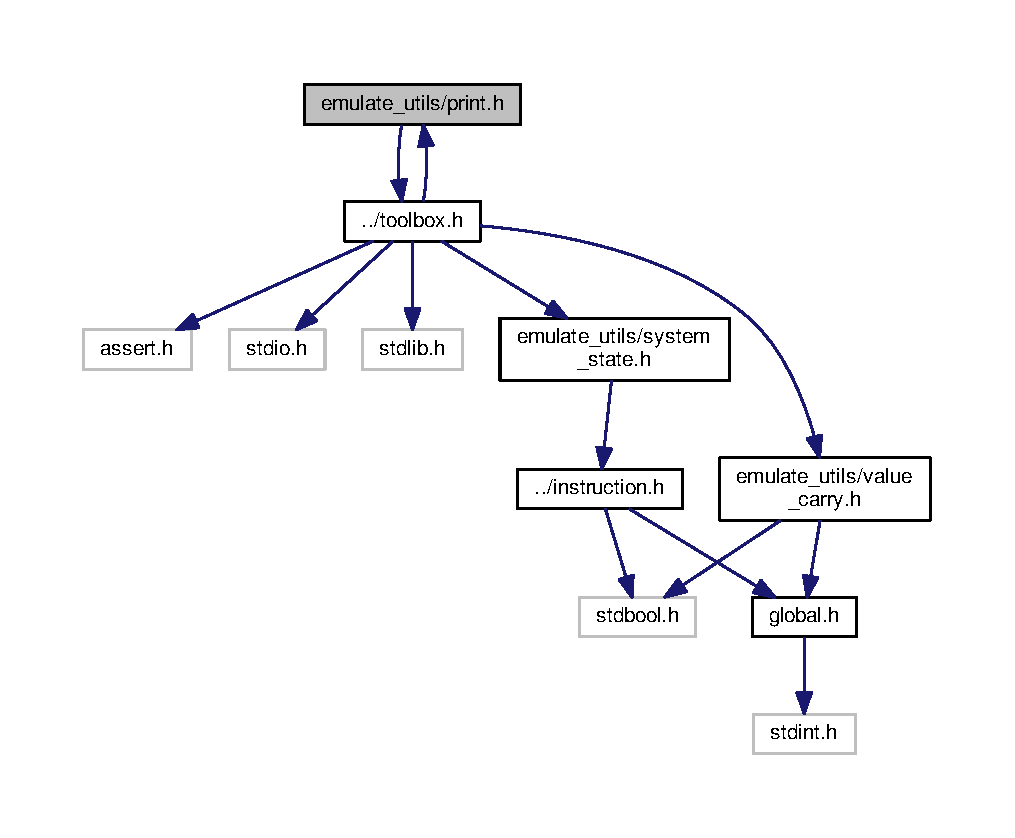
\includegraphics[width=350pt]{print_8h__incl}
\end{center}
\end{figure}
This graph shows which files directly or indirectly include this file\+:\nopagebreak
\begin{figure}[H]
\begin{center}
\leavevmode
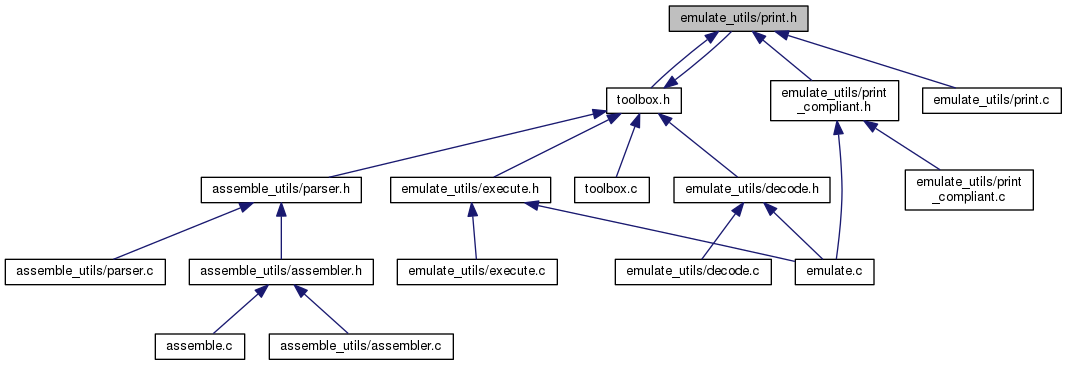
\includegraphics[width=350pt]{print_8h__dep__incl}
\end{center}
\end{figure}
\subsection*{Functions}
\begin{DoxyCompactItemize}
\item 
void \hyperlink{print_8h_aa6201dccc033aad617c0d854e18f0915}{print\+\_\+array} (\hyperlink{global_8h_a0661d7d1353e0bca70c64563f635b034}{byte\+\_\+t} $\ast$memory, size\+\_\+t bytes\+\_\+to\+\_\+print)
\begin{DoxyCompactList}\small\item\em Prints a given number of bytes, from an array of bytes. \end{DoxyCompactList}\item 
void \hyperlink{print_8h_ae3374a188808236ad908ca5300516ae6}{print\+\_\+system\+\_\+state} (\hyperlink{structsystem__state__t}{system\+\_\+state\+\_\+t} $\ast$machine)
\begin{DoxyCompactList}\small\item\em Prints system state details. \end{DoxyCompactList}\item 
void \hyperlink{print_8h_aa0d2fa15c6ec7ec862fb74640427e510}{print\+\_\+registers} (\hyperlink{structsystem__state__t}{system\+\_\+state\+\_\+t} $\ast$machine)
\begin{DoxyCompactList}\small\item\em Prints the values of registers. \end{DoxyCompactList}\item 
void \hyperlink{print_8h_a19bd450ad0dc7d7d873f9add3989c0b5}{print\+\_\+memory} (\hyperlink{structsystem__state__t}{system\+\_\+state\+\_\+t} $\ast$machine)
\begin{DoxyCompactList}\small\item\em Prints any non-\/zero words from memory. \end{DoxyCompactList}\item 
void \hyperlink{print_8h_a48a0096457ff1ab2d250b08778a5c4a2}{print\+\_\+decoded\+\_\+instruction} (\hyperlink{structsystem__state__t}{system\+\_\+state\+\_\+t} $\ast$machine)
\begin{DoxyCompactList}\small\item\em Prints details for the decoded instruction. \end{DoxyCompactList}\item 
void \hyperlink{print_8h_add0d5aaad07992e7c0b0f956255e07ac}{print\+\_\+fetched\+\_\+instruction} (\hyperlink{structsystem__state__t}{system\+\_\+state\+\_\+t} $\ast$machine)
\begin{DoxyCompactList}\small\item\em Prints the fetched instruction, if present. \end{DoxyCompactList}\item 
void \hyperlink{print_8h_a09f4c8695471e9d40ec8b728462e0bfa}{print\+\_\+instruction} (\hyperlink{structinstruction__t}{instruction\+\_\+t} $\ast$instruction)
\begin{DoxyCompactList}\small\item\em Prints details for the instruction. \end{DoxyCompactList}\item 
void \hyperlink{print_8h_aa2768353c6d59470774fc648d3e7496f}{print\+\_\+value} (\hyperlink{global_8h_a0e7744482eed560726581dae7d3cb8b2}{word\+\_\+t} value)
\begin{DoxyCompactList}\small\item\em Prints a value for debugging, in binary, hex and 2\textquotesingle{}s complement. \end{DoxyCompactList}\item 
char $\ast$ \hyperlink{print_8h_afc0249cb12aa211e3118266c4ad1741a}{get\+\_\+cond} (\hyperlink{global_8h_a57ba194eedfb8000c1a101fd42abdcf2}{condition\+\_\+t} cond)
\begin{DoxyCompactList}\small\item\em Returns the string representing the condition type. \end{DoxyCompactList}\item 
char $\ast$ \hyperlink{print_8h_abf595da7fda4726194ee1cc915cfd317}{get\+\_\+opcode} (\hyperlink{global_8h_a8d0559dcae6e251ff5663e79d5581c7d}{opcode\+\_\+t} operation)
\begin{DoxyCompactList}\small\item\em Returns the string representing the opcode. \end{DoxyCompactList}\item 
char $\ast$ \hyperlink{print_8h_a7e0f497b13f42696447d87ab77800073}{get\+\_\+shift} (\hyperlink{global_8h_a22746cb89e8b2ed0a61876e36446f37f}{shift\+\_\+t} shift)
\begin{DoxyCompactList}\small\item\em Returns the string representing the shift type. \end{DoxyCompactList}\item 
void \hyperlink{print_8h_a111c6b9bb0e71ed6dcb2841b43821224}{print\+\_\+binary\+\_\+value} (\hyperlink{global_8h_a0e7744482eed560726581dae7d3cb8b2}{word\+\_\+t} value)
\begin{DoxyCompactList}\small\item\em Prints the padded binary representation of value. \end{DoxyCompactList}\end{DoxyCompactItemize}


\subsection{Detailed Description}
Header file for \hyperlink{print_8c}{print.\+c}. 



\subsection{Function Documentation}
\index{print.\+h@{print.\+h}!get\+\_\+cond@{get\+\_\+cond}}
\index{get\+\_\+cond@{get\+\_\+cond}!print.\+h@{print.\+h}}
\subsubsection[{\texorpdfstring{get\+\_\+cond(condition\+\_\+t cond)}{get_cond(condition_t cond)}}]{\setlength{\rightskip}{0pt plus 5cm}char$\ast$ get\+\_\+cond (
\begin{DoxyParamCaption}
\item[{{\bf condition\+\_\+t}}]{cond}
\end{DoxyParamCaption}
)}\hypertarget{print_8h_afc0249cb12aa211e3118266c4ad1741a}{}\label{print_8h_afc0249cb12aa211e3118266c4ad1741a}


Returns the string representing the condition type. 


\begin{DoxyParams}{Parameters}
{\em cond} & The condition type. \\
\hline
\end{DoxyParams}
\begin{DoxyReturn}{Returns}
The string of the condition type for printing. 
\end{DoxyReturn}
\index{print.\+h@{print.\+h}!get\+\_\+opcode@{get\+\_\+opcode}}
\index{get\+\_\+opcode@{get\+\_\+opcode}!print.\+h@{print.\+h}}
\subsubsection[{\texorpdfstring{get\+\_\+opcode(opcode\+\_\+t operation)}{get_opcode(opcode_t operation)}}]{\setlength{\rightskip}{0pt plus 5cm}char$\ast$ get\+\_\+opcode (
\begin{DoxyParamCaption}
\item[{{\bf opcode\+\_\+t}}]{operation}
\end{DoxyParamCaption}
)}\hypertarget{print_8h_abf595da7fda4726194ee1cc915cfd317}{}\label{print_8h_abf595da7fda4726194ee1cc915cfd317}


Returns the string representing the opcode. 


\begin{DoxyParams}{Parameters}
{\em operation} & The opcode. \\
\hline
\end{DoxyParams}
\begin{DoxyReturn}{Returns}
The string of the opcode for printing. 
\end{DoxyReturn}
\index{print.\+h@{print.\+h}!get\+\_\+shift@{get\+\_\+shift}}
\index{get\+\_\+shift@{get\+\_\+shift}!print.\+h@{print.\+h}}
\subsubsection[{\texorpdfstring{get\+\_\+shift(shift\+\_\+t shift)}{get_shift(shift_t shift)}}]{\setlength{\rightskip}{0pt plus 5cm}char$\ast$ get\+\_\+shift (
\begin{DoxyParamCaption}
\item[{{\bf shift\+\_\+t}}]{shift}
\end{DoxyParamCaption}
)}\hypertarget{print_8h_a7e0f497b13f42696447d87ab77800073}{}\label{print_8h_a7e0f497b13f42696447d87ab77800073}


Returns the string representing the shift type. 


\begin{DoxyParams}{Parameters}
{\em operation} & The type of shift. \\
\hline
\end{DoxyParams}
\begin{DoxyReturn}{Returns}
The string of the type of shift for printing. 
\end{DoxyReturn}
\index{print.\+h@{print.\+h}!print\+\_\+array@{print\+\_\+array}}
\index{print\+\_\+array@{print\+\_\+array}!print.\+h@{print.\+h}}
\subsubsection[{\texorpdfstring{print\+\_\+array(byte\+\_\+t $\ast$memory, size\+\_\+t bytes\+\_\+to\+\_\+print)}{print_array(byte_t *memory, size_t bytes_to_print)}}]{\setlength{\rightskip}{0pt plus 5cm}void print\+\_\+array (
\begin{DoxyParamCaption}
\item[{{\bf byte\+\_\+t} $\ast$}]{memory, }
\item[{size\+\_\+t}]{bytes\+\_\+to\+\_\+print}
\end{DoxyParamCaption}
)}\hypertarget{print_8h_aa6201dccc033aad617c0d854e18f0915}{}\label{print_8h_aa6201dccc033aad617c0d854e18f0915}


Prints a given number of bytes, from an array of bytes. 

Prints a given number bytes from memory, starting from address 0. Lines are broken every word (4 bytes). Useful for debugging. 
\begin{DoxyParams}{Parameters}
{\em memory} & An array of bytes to print. \\
\hline
{\em bytes\+\_\+to\+\_\+print} & The number of bytes to print (from 0). \\
\hline
\end{DoxyParams}
\index{print.\+h@{print.\+h}!print\+\_\+binary\+\_\+value@{print\+\_\+binary\+\_\+value}}
\index{print\+\_\+binary\+\_\+value@{print\+\_\+binary\+\_\+value}!print.\+h@{print.\+h}}
\subsubsection[{\texorpdfstring{print\+\_\+binary\+\_\+value(word\+\_\+t value)}{print_binary_value(word_t value)}}]{\setlength{\rightskip}{0pt plus 5cm}void print\+\_\+binary\+\_\+value (
\begin{DoxyParamCaption}
\item[{{\bf word\+\_\+t}}]{value}
\end{DoxyParamCaption}
)}\hypertarget{print_8h_a111c6b9bb0e71ed6dcb2841b43821224}{}\label{print_8h_a111c6b9bb0e71ed6dcb2841b43821224}


Prints the padded binary representation of value. 

Prints W\+O\+R\+D\+\_\+\+S\+I\+ZE bits. 
\begin{DoxyParams}{Parameters}
{\em value} & The word for printing. \\
\hline
\end{DoxyParams}
\index{print.\+h@{print.\+h}!print\+\_\+decoded\+\_\+instruction@{print\+\_\+decoded\+\_\+instruction}}
\index{print\+\_\+decoded\+\_\+instruction@{print\+\_\+decoded\+\_\+instruction}!print.\+h@{print.\+h}}
\subsubsection[{\texorpdfstring{print\+\_\+decoded\+\_\+instruction(system\+\_\+state\+\_\+t $\ast$machine)}{print_decoded_instruction(system_state_t *machine)}}]{\setlength{\rightskip}{0pt plus 5cm}void print\+\_\+decoded\+\_\+instruction (
\begin{DoxyParamCaption}
\item[{{\bf system\+\_\+state\+\_\+t} $\ast$}]{machine}
\end{DoxyParamCaption}
)}\hypertarget{print_8h_a48a0096457ff1ab2d250b08778a5c4a2}{}\label{print_8h_a48a0096457ff1ab2d250b08778a5c4a2}


Prints details for the decoded instruction. 

Prints the type of the instruction, and any details required\+:
\begin{DoxyItemize}
\item For branch instructions, prints the condition and the offset.
\item For multiply instructions, prints the condition, flags and registers.
\item For data processing instructions, prints the condition, flags, opcodes, operands, and shift information.
\item For single data transfer instructions, prints flags, registers and offset. 
\begin{DoxyParams}{Parameters}
{\em machine} & The current system state. \\
\hline
\end{DoxyParams}

\end{DoxyItemize}\index{print.\+h@{print.\+h}!print\+\_\+fetched\+\_\+instruction@{print\+\_\+fetched\+\_\+instruction}}
\index{print\+\_\+fetched\+\_\+instruction@{print\+\_\+fetched\+\_\+instruction}!print.\+h@{print.\+h}}
\subsubsection[{\texorpdfstring{print\+\_\+fetched\+\_\+instruction(system\+\_\+state\+\_\+t $\ast$machine)}{print_fetched_instruction(system_state_t *machine)}}]{\setlength{\rightskip}{0pt plus 5cm}void print\+\_\+fetched\+\_\+instruction (
\begin{DoxyParamCaption}
\item[{{\bf system\+\_\+state\+\_\+t} $\ast$}]{machine}
\end{DoxyParamCaption}
)}\hypertarget{print_8h_add0d5aaad07992e7c0b0f956255e07ac}{}\label{print_8h_add0d5aaad07992e7c0b0f956255e07ac}


Prints the fetched instruction, if present. 


\begin{DoxyParams}{Parameters}
{\em machine} & The current system state. \\
\hline
\end{DoxyParams}
\index{print.\+h@{print.\+h}!print\+\_\+instruction@{print\+\_\+instruction}}
\index{print\+\_\+instruction@{print\+\_\+instruction}!print.\+h@{print.\+h}}
\subsubsection[{\texorpdfstring{print\+\_\+instruction(instruction\+\_\+t $\ast$instruction)}{print_instruction(instruction_t *instruction)}}]{\setlength{\rightskip}{0pt plus 5cm}void print\+\_\+instruction (
\begin{DoxyParamCaption}
\item[{{\bf instruction\+\_\+t} $\ast$}]{instruction}
\end{DoxyParamCaption}
)}\hypertarget{print_8h_a09f4c8695471e9d40ec8b728462e0bfa}{}\label{print_8h_a09f4c8695471e9d40ec8b728462e0bfa}


Prints details for the instruction. 

Prints the type of the instruction, and any details required\+:
\begin{DoxyItemize}
\item For branch instructions, prints the condition and the offset.
\item For multiply instructions, prints the condition, flags and registers.
\item For data processing instructions, prints the condition, flags, opcodes, operands, and shift information.
\item For single data transfer instructions, prints flags, registers and offset. 
\begin{DoxyParams}{Parameters}
{\em instruction} & The instruction. \\
\hline
\end{DoxyParams}

\end{DoxyItemize}\index{print.\+h@{print.\+h}!print\+\_\+memory@{print\+\_\+memory}}
\index{print\+\_\+memory@{print\+\_\+memory}!print.\+h@{print.\+h}}
\subsubsection[{\texorpdfstring{print\+\_\+memory(system\+\_\+state\+\_\+t $\ast$machine)}{print_memory(system_state_t *machine)}}]{\setlength{\rightskip}{0pt plus 5cm}void print\+\_\+memory (
\begin{DoxyParamCaption}
\item[{{\bf system\+\_\+state\+\_\+t} $\ast$}]{machine}
\end{DoxyParamCaption}
)}\hypertarget{print_8h_a19bd450ad0dc7d7d873f9add3989c0b5}{}\label{print_8h_a19bd450ad0dc7d7d873f9add3989c0b5}


Prints any non-\/zero words from memory. 

Prints any non-\/zero words from memory and their addresses. 
\begin{DoxyParams}{Parameters}
{\em machine} & The current system state. \\
\hline
\end{DoxyParams}
\index{print.\+h@{print.\+h}!print\+\_\+registers@{print\+\_\+registers}}
\index{print\+\_\+registers@{print\+\_\+registers}!print.\+h@{print.\+h}}
\subsubsection[{\texorpdfstring{print\+\_\+registers(system\+\_\+state\+\_\+t $\ast$machine)}{print_registers(system_state_t *machine)}}]{\setlength{\rightskip}{0pt plus 5cm}void print\+\_\+registers (
\begin{DoxyParamCaption}
\item[{{\bf system\+\_\+state\+\_\+t} $\ast$}]{machine}
\end{DoxyParamCaption}
)}\hypertarget{print_8h_aa0d2fa15c6ec7ec862fb74640427e510}{}\label{print_8h_aa0d2fa15c6ec7ec862fb74640427e510}


Prints the values of registers. 

Prints the values held in each of the N\+U\+M\+\_\+\+R\+E\+G\+I\+S\+T\+E\+RS registers. 
\begin{DoxyParams}{Parameters}
{\em machine} & The current system state. \\
\hline
\end{DoxyParams}
\index{print.\+h@{print.\+h}!print\+\_\+system\+\_\+state@{print\+\_\+system\+\_\+state}}
\index{print\+\_\+system\+\_\+state@{print\+\_\+system\+\_\+state}!print.\+h@{print.\+h}}
\subsubsection[{\texorpdfstring{print\+\_\+system\+\_\+state(system\+\_\+state\+\_\+t $\ast$machine)}{print_system_state(system_state_t *machine)}}]{\setlength{\rightskip}{0pt plus 5cm}void print\+\_\+system\+\_\+state (
\begin{DoxyParamCaption}
\item[{{\bf system\+\_\+state\+\_\+t} $\ast$}]{machine}
\end{DoxyParamCaption}
)}\hypertarget{print_8h_ae3374a188808236ad908ca5300516ae6}{}\label{print_8h_ae3374a188808236ad908ca5300516ae6}


Prints system state details. 

Prints the current system state. Prints all register values, any memory values which are not 0, the decoded instruction and the fetched instruction. 
\begin{DoxyParams}{Parameters}
{\em machine} & The current system state. \\
\hline
\end{DoxyParams}
\index{print.\+h@{print.\+h}!print\+\_\+value@{print\+\_\+value}}
\index{print\+\_\+value@{print\+\_\+value}!print.\+h@{print.\+h}}
\subsubsection[{\texorpdfstring{print\+\_\+value(word\+\_\+t value)}{print_value(word_t value)}}]{\setlength{\rightskip}{0pt plus 5cm}void print\+\_\+value (
\begin{DoxyParamCaption}
\item[{{\bf word\+\_\+t}}]{value}
\end{DoxyParamCaption}
)}\hypertarget{print_8h_aa2768353c6d59470774fc648d3e7496f}{}\label{print_8h_aa2768353c6d59470774fc648d3e7496f}


Prints a value for debugging, in binary, hex and 2\textquotesingle{}s complement. 


\begin{DoxyParams}{Parameters}
{\em value} & The word to print. \\
\hline
\end{DoxyParams}

\hypertarget{print__compliant_8c}{}\section{emulate\+\_\+utils/print\+\_\+compliant.c File Reference}
\label{print__compliant_8c}\index{emulate\+\_\+utils/print\+\_\+compliant.\+c@{emulate\+\_\+utils/print\+\_\+compliant.\+c}}


Functions for printing system details to match test cases.  


{\ttfamily \#include \char`\"{}print\+\_\+compliant.\+h\char`\"{}}\\*
Include dependency graph for print\+\_\+compliant.\+c\+:\nopagebreak
\begin{figure}[H]
\begin{center}
\leavevmode
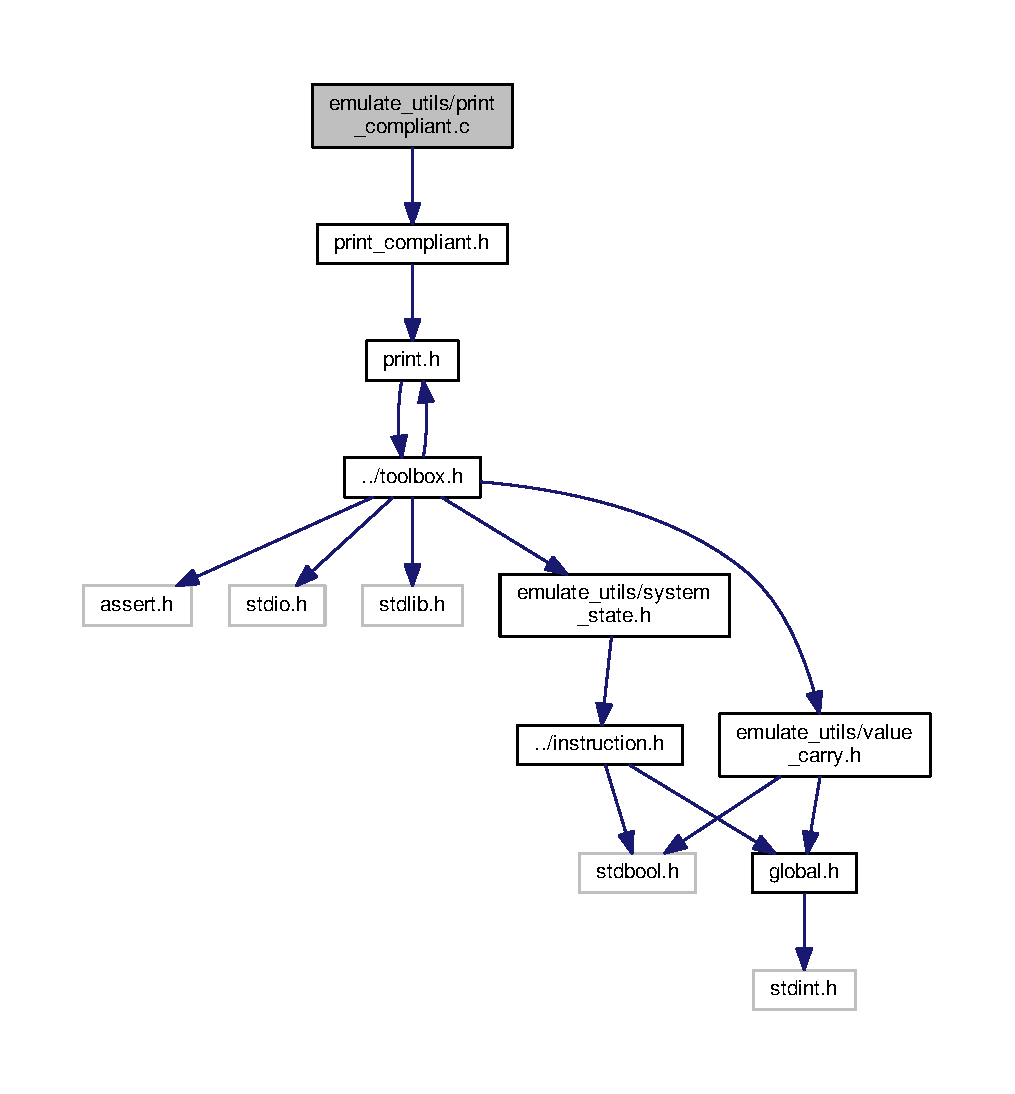
\includegraphics[width=350pt]{print__compliant_8c__incl}
\end{center}
\end{figure}
\subsection*{Functions}
\begin{DoxyCompactItemize}
\item 
void \hyperlink{print__compliant_8c_a53e74af552445098554650a9cd55871d}{print\+\_\+system\+\_\+state\+\_\+compliant} (\hyperlink{structsystem__state__t}{system\+\_\+state\+\_\+t} $\ast$machine)
\begin{DoxyCompactList}\small\item\em Prints system state details for test cases. \end{DoxyCompactList}\item 
void \hyperlink{print__compliant_8c_aec17ac1dfe2ed696d104fda9a65359e4}{print\+\_\+registers\+\_\+compliant} (\hyperlink{structsystem__state__t}{system\+\_\+state\+\_\+t} $\ast$machine)
\begin{DoxyCompactList}\small\item\em Prints the values of the registers of the machine for test cases. \end{DoxyCompactList}\item 
void \hyperlink{print__compliant_8c_aa8b4d6004e6a83724b3af18db9ca31a4}{print\+\_\+memory\+\_\+compliant} (\hyperlink{structsystem__state__t}{system\+\_\+state\+\_\+t} $\ast$machine)
\begin{DoxyCompactList}\small\item\em Prints non-\/zero memory entries for test cases. \end{DoxyCompactList}\item 
void \hyperlink{print__compliant_8c_abe651d4f119a46084e83caed390671b9}{print\+\_\+value\+\_\+compliant} (\hyperlink{global_8h_a0e7744482eed560726581dae7d3cb8b2}{word\+\_\+t} value)
\begin{DoxyCompactList}\small\item\em Prints a value for test cases, in hex and two\textquotesingle{}s complement. \end{DoxyCompactList}\end{DoxyCompactItemize}


\subsection{Detailed Description}
Functions for printing system details to match test cases. 



\subsection{Function Documentation}
\index{print\+\_\+compliant.\+c@{print\+\_\+compliant.\+c}!print\+\_\+memory\+\_\+compliant@{print\+\_\+memory\+\_\+compliant}}
\index{print\+\_\+memory\+\_\+compliant@{print\+\_\+memory\+\_\+compliant}!print\+\_\+compliant.\+c@{print\+\_\+compliant.\+c}}
\subsubsection[{\texorpdfstring{print\+\_\+memory\+\_\+compliant(system\+\_\+state\+\_\+t $\ast$machine)}{print_memory_compliant(system_state_t *machine)}}]{\setlength{\rightskip}{0pt plus 5cm}void print\+\_\+memory\+\_\+compliant (
\begin{DoxyParamCaption}
\item[{{\bf system\+\_\+state\+\_\+t} $\ast$}]{machine}
\end{DoxyParamCaption}
)}\hypertarget{print__compliant_8c_aa8b4d6004e6a83724b3af18db9ca31a4}{}\label{print__compliant_8c_aa8b4d6004e6a83724b3af18db9ca31a4}


Prints non-\/zero memory entries for test cases. 


\begin{DoxyParams}{Parameters}
{\em machine} & The current system state. \\
\hline
\end{DoxyParams}
\index{print\+\_\+compliant.\+c@{print\+\_\+compliant.\+c}!print\+\_\+registers\+\_\+compliant@{print\+\_\+registers\+\_\+compliant}}
\index{print\+\_\+registers\+\_\+compliant@{print\+\_\+registers\+\_\+compliant}!print\+\_\+compliant.\+c@{print\+\_\+compliant.\+c}}
\subsubsection[{\texorpdfstring{print\+\_\+registers\+\_\+compliant(system\+\_\+state\+\_\+t $\ast$machine)}{print_registers_compliant(system_state_t *machine)}}]{\setlength{\rightskip}{0pt plus 5cm}void print\+\_\+registers\+\_\+compliant (
\begin{DoxyParamCaption}
\item[{{\bf system\+\_\+state\+\_\+t} $\ast$}]{machine}
\end{DoxyParamCaption}
)}\hypertarget{print__compliant_8c_aec17ac1dfe2ed696d104fda9a65359e4}{}\label{print__compliant_8c_aec17ac1dfe2ed696d104fda9a65359e4}


Prints the values of the registers of the machine for test cases. 


\begin{DoxyParams}{Parameters}
{\em machine} & The current system state. \\
\hline
\end{DoxyParams}
\index{print\+\_\+compliant.\+c@{print\+\_\+compliant.\+c}!print\+\_\+system\+\_\+state\+\_\+compliant@{print\+\_\+system\+\_\+state\+\_\+compliant}}
\index{print\+\_\+system\+\_\+state\+\_\+compliant@{print\+\_\+system\+\_\+state\+\_\+compliant}!print\+\_\+compliant.\+c@{print\+\_\+compliant.\+c}}
\subsubsection[{\texorpdfstring{print\+\_\+system\+\_\+state\+\_\+compliant(system\+\_\+state\+\_\+t $\ast$machine)}{print_system_state_compliant(system_state_t *machine)}}]{\setlength{\rightskip}{0pt plus 5cm}void print\+\_\+system\+\_\+state\+\_\+compliant (
\begin{DoxyParamCaption}
\item[{{\bf system\+\_\+state\+\_\+t} $\ast$}]{machine}
\end{DoxyParamCaption}
)}\hypertarget{print__compliant_8c_a53e74af552445098554650a9cd55871d}{}\label{print__compliant_8c_a53e74af552445098554650a9cd55871d}


Prints system state details for test cases. 

Prints the current system state. Prints all register values, any memory values which are not 0. Prints in test case format. 
\begin{DoxyParams}{Parameters}
{\em machine} & The current system state. \\
\hline
\end{DoxyParams}
\index{print\+\_\+compliant.\+c@{print\+\_\+compliant.\+c}!print\+\_\+value\+\_\+compliant@{print\+\_\+value\+\_\+compliant}}
\index{print\+\_\+value\+\_\+compliant@{print\+\_\+value\+\_\+compliant}!print\+\_\+compliant.\+c@{print\+\_\+compliant.\+c}}
\subsubsection[{\texorpdfstring{print\+\_\+value\+\_\+compliant(word\+\_\+t value)}{print_value_compliant(word_t value)}}]{\setlength{\rightskip}{0pt plus 5cm}void print\+\_\+value\+\_\+compliant (
\begin{DoxyParamCaption}
\item[{{\bf word\+\_\+t}}]{value}
\end{DoxyParamCaption}
)}\hypertarget{print__compliant_8c_abe651d4f119a46084e83caed390671b9}{}\label{print__compliant_8c_abe651d4f119a46084e83caed390671b9}


Prints a value for test cases, in hex and two\textquotesingle{}s complement. 


\begin{DoxyParams}{Parameters}
{\em value} & The word to print. \\
\hline
\end{DoxyParams}

\hypertarget{print__compliant_8h}{}\section{emulate\+\_\+utils/print\+\_\+compliant.h File Reference}
\label{print__compliant_8h}\index{emulate\+\_\+utils/print\+\_\+compliant.\+h@{emulate\+\_\+utils/print\+\_\+compliant.\+h}}


Header file for \hyperlink{print__compliant_8c}{print\+\_\+compliant.\+c}.  


{\ttfamily \#include \char`\"{}print.\+h\char`\"{}}\\*
Include dependency graph for print\+\_\+compliant.\+h\+:
\nopagebreak
\begin{figure}[H]
\begin{center}
\leavevmode
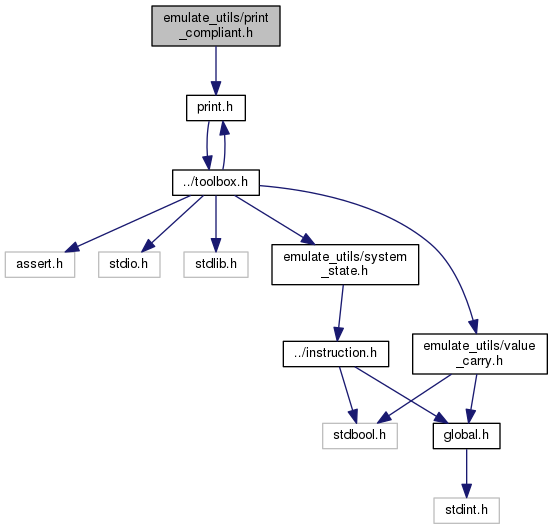
\includegraphics[width=350pt]{print__compliant_8h__incl}
\end{center}
\end{figure}
This graph shows which files directly or indirectly include this file\+:
\nopagebreak
\begin{figure}[H]
\begin{center}
\leavevmode
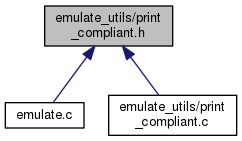
\includegraphics[width=254pt]{print__compliant_8h__dep__incl}
\end{center}
\end{figure}
\subsection*{Functions}
\begin{DoxyCompactItemize}
\item 
void \hyperlink{print__compliant_8h_a53e74af552445098554650a9cd55871d}{print\+\_\+system\+\_\+state\+\_\+compliant} (\hyperlink{structsystem__state__t}{system\+\_\+state\+\_\+t} $\ast$machine)
\begin{DoxyCompactList}\small\item\em Prints system state details for test cases. \end{DoxyCompactList}\end{DoxyCompactItemize}


\subsection{Detailed Description}
Header file for \hyperlink{print__compliant_8c}{print\+\_\+compliant.\+c}. 



\subsection{Function Documentation}
\index{print\+\_\+compliant.\+h@{print\+\_\+compliant.\+h}!print\+\_\+system\+\_\+state\+\_\+compliant@{print\+\_\+system\+\_\+state\+\_\+compliant}}
\index{print\+\_\+system\+\_\+state\+\_\+compliant@{print\+\_\+system\+\_\+state\+\_\+compliant}!print\+\_\+compliant.\+h@{print\+\_\+compliant.\+h}}
\subsubsection[{\texorpdfstring{print\+\_\+system\+\_\+state\+\_\+compliant(system\+\_\+state\+\_\+t $\ast$machine)}{print_system_state_compliant(system_state_t *machine)}}]{\setlength{\rightskip}{0pt plus 5cm}void print\+\_\+system\+\_\+state\+\_\+compliant (
\begin{DoxyParamCaption}
\item[{{\bf system\+\_\+state\+\_\+t} $\ast$}]{machine}
\end{DoxyParamCaption}
)}\hypertarget{print__compliant_8h_a53e74af552445098554650a9cd55871d}{}\label{print__compliant_8h_a53e74af552445098554650a9cd55871d}


Prints system state details for test cases. 

Prints the current system state. Prints all register values, any memory values which are not 0. Prints in test case format. 
\begin{DoxyParams}{Parameters}
{\em machine} & The current system state. \\
\hline
\end{DoxyParams}

\hypertarget{system__state_8h}{}\section{emulate\+\_\+utils/system\+\_\+state.h File Reference}
\label{system__state_8h}\index{emulate\+\_\+utils/system\+\_\+state.\+h@{emulate\+\_\+utils/system\+\_\+state.\+h}}


A header to define the \hyperlink{structsystem__state__t}{system\+\_\+state\+\_\+t} type.  


{\ttfamily \#include \char`\"{}../instruction.\+h\char`\"{}}\\*
Include dependency graph for system\+\_\+state.\+h\+:\nopagebreak
\begin{figure}[H]
\begin{center}
\leavevmode
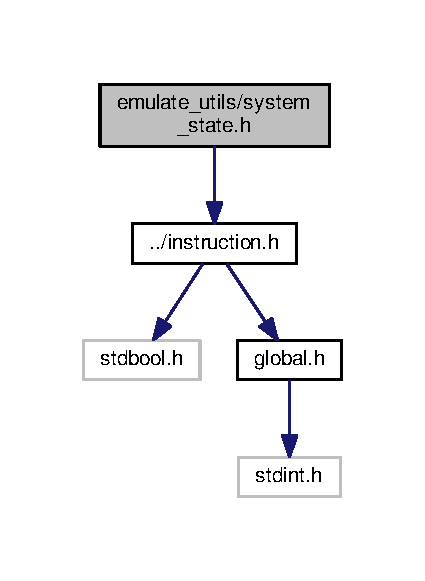
\includegraphics[width=204pt]{system__state_8h__incl}
\end{center}
\end{figure}
This graph shows which files directly or indirectly include this file\+:\nopagebreak
\begin{figure}[H]
\begin{center}
\leavevmode
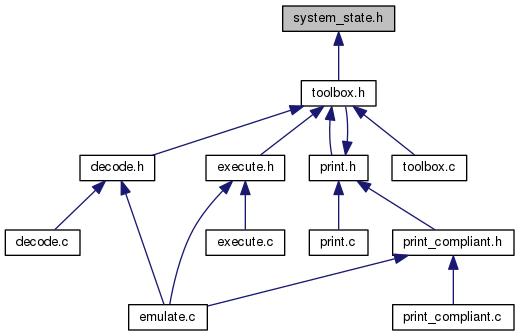
\includegraphics[width=350pt]{system__state_8h__dep__incl}
\end{center}
\end{figure}
\subsection*{Data Structures}
\begin{DoxyCompactItemize}
\item 
struct \hyperlink{structsystem__state__t}{system\+\_\+state\+\_\+t}
\begin{DoxyCompactList}\small\item\em A struct that holds information about the current system state. \end{DoxyCompactList}\end{DoxyCompactItemize}


\subsection{Detailed Description}
A header to define the \hyperlink{structsystem__state__t}{system\+\_\+state\+\_\+t} type. 


\hypertarget{toolbox_8c}{}\section{toolbox.\+c File Reference}
\label{toolbox_8c}\index{toolbox.\+c@{toolbox.\+c}}


Miscellaneous functions that are widely used throughout the code.  


{\ttfamily \#include \char`\"{}toolbox.\+h\char`\"{}}\\*
Include dependency graph for toolbox.\+c\+:
\nopagebreak
\begin{figure}[H]
\begin{center}
\leavevmode
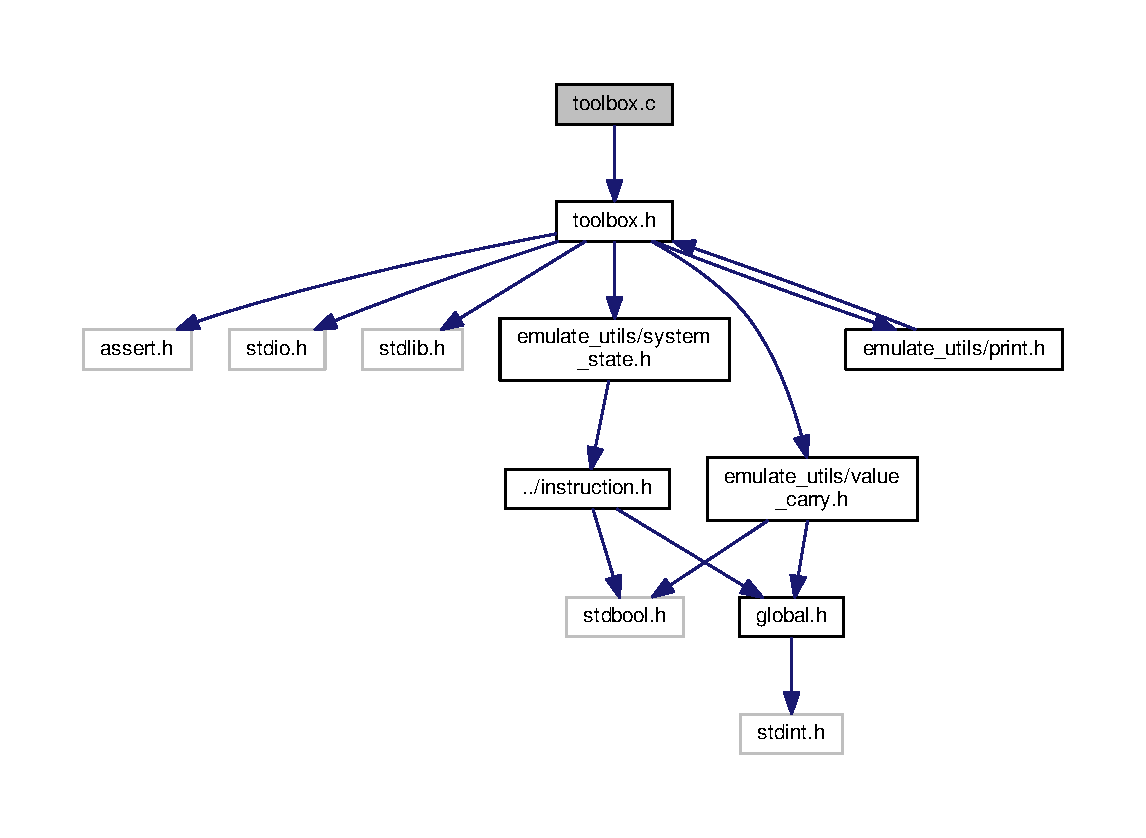
\includegraphics[width=350pt]{toolbox_8c__incl}
\end{center}
\end{figure}
\subsection*{Functions}
\begin{DoxyCompactItemize}
\item 
void \hyperlink{toolbox_8c_a6d650fb79ff7ee7fe331286272a0f794}{load\+\_\+file} (char $\ast$fname, \hyperlink{global_8h_a0661d7d1353e0bca70c64563f635b034}{byte\+\_\+t} $\ast$memory)
\begin{DoxyCompactList}\small\item\em Loads a binary file into the memory. \end{DoxyCompactList}\item 
void \hyperlink{toolbox_8c_a7309491724696785ff2df97b88dbc69d}{exit\+\_\+program} (\hyperlink{structsystem__state__t}{system\+\_\+state\+\_\+t} $\ast$machine)
\begin{DoxyCompactList}\small\item\em Exits gracefully. \end{DoxyCompactList}\item 
\hyperlink{global_8h_a0e7744482eed560726581dae7d3cb8b2}{word\+\_\+t} \hyperlink{toolbox_8c_ae00c97fb61caa5c5a327f53743671ea7}{get\+\_\+word} (\hyperlink{structsystem__state__t}{system\+\_\+state\+\_\+t} $\ast$machine, uint32\+\_\+t mem\+\_\+address)
\begin{DoxyCompactList}\small\item\em Gets a memory word from a given address. \end{DoxyCompactList}\item 
\hyperlink{global_8h_a0e7744482eed560726581dae7d3cb8b2}{word\+\_\+t} \hyperlink{toolbox_8c_a6418bf675c48b3820635a6010b83a159}{get\+\_\+word\+\_\+compliant} (\hyperlink{structsystem__state__t}{system\+\_\+state\+\_\+t} $\ast$machine, \hyperlink{global_8h_a8f4b132f56a25431714862229639be12}{address\+\_\+t} mem\+\_\+address)
\begin{DoxyCompactList}\small\item\em Gets a memory word from a given address (for printing only). \end{DoxyCompactList}\item 
void \hyperlink{toolbox_8c_a17194b5825208d2a4d7c9e266b5fdbc2}{set\+\_\+word} (\hyperlink{structsystem__state__t}{system\+\_\+state\+\_\+t} $\ast$machine, uint32\+\_\+t mem\+\_\+address, \hyperlink{global_8h_a0e7744482eed560726581dae7d3cb8b2}{word\+\_\+t} word)
\begin{DoxyCompactList}\small\item\em Writes a word to memory at a given address. \end{DoxyCompactList}\item 
\hyperlink{global_8h_a0e7744482eed560726581dae7d3cb8b2}{word\+\_\+t} \hyperlink{toolbox_8c_a686137c6e030fbf3387fda07e8eeb085}{negate} (\hyperlink{global_8h_a0e7744482eed560726581dae7d3cb8b2}{word\+\_\+t} value)
\begin{DoxyCompactList}\small\item\em Negates a two\textquotesingle{}s complement value. \end{DoxyCompactList}\item 
bool \hyperlink{toolbox_8c_a0d865a08414b59081c1cbb7787816445}{is\+\_\+negative} (\hyperlink{global_8h_a0e7744482eed560726581dae7d3cb8b2}{word\+\_\+t} value)
\begin{DoxyCompactList}\small\item\em Returns true iff two\textquotesingle{}s complement value is negative. \end{DoxyCompactList}\item 
\hyperlink{global_8h_a0e7744482eed560726581dae7d3cb8b2}{word\+\_\+t} \hyperlink{toolbox_8c_a8c2b56d7b4c74bd125678cf3a1b1f418}{absolute} (\hyperlink{global_8h_a0e7744482eed560726581dae7d3cb8b2}{word\+\_\+t} value)
\begin{DoxyCompactList}\small\item\em Returns absolute two\textquotesingle{}s complement value. \end{DoxyCompactList}\item 
\hyperlink{structvalue__carry__t}{value\+\_\+carry\+\_\+t} $\ast$ \hyperlink{toolbox_8c_a519bda814c2b3d1f57613e56de5214b8}{shifter} (\hyperlink{global_8h_a22746cb89e8b2ed0a61876e36446f37f}{shift\+\_\+t} type, \hyperlink{global_8h_a0e7744482eed560726581dae7d3cb8b2}{word\+\_\+t} shift\+\_\+amount, \hyperlink{global_8h_a0e7744482eed560726581dae7d3cb8b2}{word\+\_\+t} value)
\begin{DoxyCompactList}\small\item\em Shifts a value and returns a pointer. \end{DoxyCompactList}\end{DoxyCompactItemize}


\subsection{Detailed Description}
Miscellaneous functions that are widely used throughout the code. 



\subsection{Function Documentation}
\index{toolbox.\+c@{toolbox.\+c}!absolute@{absolute}}
\index{absolute@{absolute}!toolbox.\+c@{toolbox.\+c}}
\subsubsection[{\texorpdfstring{absolute(word\+\_\+t value)}{absolute(word_t value)}}]{\setlength{\rightskip}{0pt plus 5cm}{\bf word\+\_\+t} absolute (
\begin{DoxyParamCaption}
\item[{{\bf word\+\_\+t}}]{value}
\end{DoxyParamCaption}
)}\hypertarget{toolbox_8c_a8c2b56d7b4c74bd125678cf3a1b1f418}{}\label{toolbox_8c_a8c2b56d7b4c74bd125678cf3a1b1f418}


Returns absolute two\textquotesingle{}s complement value. 


\begin{DoxyParams}{Parameters}
{\em value} & A two\textquotesingle{}s complement word. \\
\hline
\end{DoxyParams}
\begin{DoxyReturn}{Returns}
The absolute value of the provided word in two\textquotesingle{}s complement. 
\end{DoxyReturn}
\index{toolbox.\+c@{toolbox.\+c}!exit\+\_\+program@{exit\+\_\+program}}
\index{exit\+\_\+program@{exit\+\_\+program}!toolbox.\+c@{toolbox.\+c}}
\subsubsection[{\texorpdfstring{exit\+\_\+program(system\+\_\+state\+\_\+t $\ast$machine)}{exit_program(system_state_t *machine)}}]{\setlength{\rightskip}{0pt plus 5cm}void exit\+\_\+program (
\begin{DoxyParamCaption}
\item[{{\bf system\+\_\+state\+\_\+t} $\ast$}]{machine}
\end{DoxyParamCaption}
)}\hypertarget{toolbox_8c_a7309491724696785ff2df97b88dbc69d}{}\label{toolbox_8c_a7309491724696785ff2df97b88dbc69d}


Exits gracefully. 

Prints the current system state, frees allocated memory and exits with a failure. To be used in the case of an error which cannot be recovered from. 
\begin{DoxyParams}{Parameters}
{\em machine} & The current system state. \\
\hline
\end{DoxyParams}
\index{toolbox.\+c@{toolbox.\+c}!get\+\_\+word@{get\+\_\+word}}
\index{get\+\_\+word@{get\+\_\+word}!toolbox.\+c@{toolbox.\+c}}
\subsubsection[{\texorpdfstring{get\+\_\+word(system\+\_\+state\+\_\+t $\ast$machine, uint32\+\_\+t mem\+\_\+address)}{get_word(system_state_t *machine, uint32_t mem_address)}}]{\setlength{\rightskip}{0pt plus 5cm}{\bf word\+\_\+t} get\+\_\+word (
\begin{DoxyParamCaption}
\item[{{\bf system\+\_\+state\+\_\+t} $\ast$}]{machine, }
\item[{uint32\+\_\+t}]{mem\+\_\+address}
\end{DoxyParamCaption}
)}\hypertarget{toolbox_8c_ae00c97fb61caa5c5a327f53743671ea7}{}\label{toolbox_8c_ae00c97fb61caa5c5a327f53743671ea7}


Gets a memory word from a given address. 


\begin{DoxyItemize}
\item If G\+P\+IO access adddress is read, prints a message to stdout.
\item If another out of bounds address is read, prints an error. 
\begin{DoxyParams}{Parameters}
{\em machine} & The current system state. \\
\hline
{\em mem\+\_\+address} & The memory address to be read from. \\
\hline
\end{DoxyParams}
\begin{DoxyReturn}{Returns}
The word at the given memory address in the current system state. 
\end{DoxyReturn}

\end{DoxyItemize}\index{toolbox.\+c@{toolbox.\+c}!get\+\_\+word\+\_\+compliant@{get\+\_\+word\+\_\+compliant}}
\index{get\+\_\+word\+\_\+compliant@{get\+\_\+word\+\_\+compliant}!toolbox.\+c@{toolbox.\+c}}
\subsubsection[{\texorpdfstring{get\+\_\+word\+\_\+compliant(system\+\_\+state\+\_\+t $\ast$machine, address\+\_\+t mem\+\_\+address)}{get_word_compliant(system_state_t *machine, address_t mem_address)}}]{\setlength{\rightskip}{0pt plus 5cm}{\bf word\+\_\+t} get\+\_\+word\+\_\+compliant (
\begin{DoxyParamCaption}
\item[{{\bf system\+\_\+state\+\_\+t} $\ast$}]{machine, }
\item[{{\bf address\+\_\+t}}]{mem\+\_\+address}
\end{DoxyParamCaption}
)}\hypertarget{toolbox_8c_a6418bf675c48b3820635a6010b83a159}{}\label{toolbox_8c_a6418bf675c48b3820635a6010b83a159}


Gets a memory word from a given address (for printing only). 

For use in compliant printing. Gets the word in little endian order. 
\begin{DoxyParams}{Parameters}
{\em machine} & The current system state. \\
\hline
{\em mem\+\_\+address} & The memory address to be read from. \\
\hline
\end{DoxyParams}
\begin{DoxyReturn}{Returns}
The word at the given memory address in the current system state. 
\end{DoxyReturn}
\index{toolbox.\+c@{toolbox.\+c}!is\+\_\+negative@{is\+\_\+negative}}
\index{is\+\_\+negative@{is\+\_\+negative}!toolbox.\+c@{toolbox.\+c}}
\subsubsection[{\texorpdfstring{is\+\_\+negative(word\+\_\+t value)}{is_negative(word_t value)}}]{\setlength{\rightskip}{0pt plus 5cm}bool is\+\_\+negative (
\begin{DoxyParamCaption}
\item[{{\bf word\+\_\+t}}]{value}
\end{DoxyParamCaption}
)}\hypertarget{toolbox_8c_a0d865a08414b59081c1cbb7787816445}{}\label{toolbox_8c_a0d865a08414b59081c1cbb7787816445}


Returns true iff two\textquotesingle{}s complement value is negative. 


\begin{DoxyParams}{Parameters}
{\em value} & A two\textquotesingle{}s complement word to check sign of. \\
\hline
\end{DoxyParams}
\begin{DoxyReturn}{Returns}
True iff provided value is negative in two\textquotesingle{}s complement. 
\end{DoxyReturn}
\index{toolbox.\+c@{toolbox.\+c}!load\+\_\+file@{load\+\_\+file}}
\index{load\+\_\+file@{load\+\_\+file}!toolbox.\+c@{toolbox.\+c}}
\subsubsection[{\texorpdfstring{load\+\_\+file(char $\ast$fname, byte\+\_\+t $\ast$memory)}{load_file(char *fname, byte_t *memory)}}]{\setlength{\rightskip}{0pt plus 5cm}void load\+\_\+file (
\begin{DoxyParamCaption}
\item[{char $\ast$}]{fname, }
\item[{{\bf byte\+\_\+t} $\ast$}]{memory}
\end{DoxyParamCaption}
)}\hypertarget{toolbox_8c_a6d650fb79ff7ee7fe331286272a0f794}{}\label{toolbox_8c_a6d650fb79ff7ee7fe331286272a0f794}


Loads a binary file into the memory. 

Writes the contents of the provided binary object code file to the memory, starting at the provided location. Returns an error message and exits if the file cannot be opened or cannot be read. 
\begin{DoxyParams}{Parameters}
{\em fname} & The filename containing object code to be loaded. \\
\hline
{\em memory} & A pointer to the first byte of memory to be written to. \\
\hline
\end{DoxyParams}
\index{toolbox.\+c@{toolbox.\+c}!negate@{negate}}
\index{negate@{negate}!toolbox.\+c@{toolbox.\+c}}
\subsubsection[{\texorpdfstring{negate(word\+\_\+t value)}{negate(word_t value)}}]{\setlength{\rightskip}{0pt plus 5cm}{\bf word\+\_\+t} negate (
\begin{DoxyParamCaption}
\item[{{\bf word\+\_\+t}}]{value}
\end{DoxyParamCaption}
)}\hypertarget{toolbox_8c_a686137c6e030fbf3387fda07e8eeb085}{}\label{toolbox_8c_a686137c6e030fbf3387fda07e8eeb085}


Negates a two\textquotesingle{}s complement value. 


\begin{DoxyParams}{Parameters}
{\em value} & The word to be negated. \\
\hline
\end{DoxyParams}
\begin{DoxyReturn}{Returns}
The negated word. 
\end{DoxyReturn}
\index{toolbox.\+c@{toolbox.\+c}!set\+\_\+word@{set\+\_\+word}}
\index{set\+\_\+word@{set\+\_\+word}!toolbox.\+c@{toolbox.\+c}}
\subsubsection[{\texorpdfstring{set\+\_\+word(system\+\_\+state\+\_\+t $\ast$machine, uint32\+\_\+t mem\+\_\+address, word\+\_\+t word)}{set_word(system_state_t *machine, uint32_t mem_address, word_t word)}}]{\setlength{\rightskip}{0pt plus 5cm}void set\+\_\+word (
\begin{DoxyParamCaption}
\item[{{\bf system\+\_\+state\+\_\+t} $\ast$}]{machine, }
\item[{uint32\+\_\+t}]{mem\+\_\+address, }
\item[{{\bf word\+\_\+t}}]{word}
\end{DoxyParamCaption}
)}\hypertarget{toolbox_8c_a17194b5825208d2a4d7c9e266b5fdbc2}{}\label{toolbox_8c_a17194b5825208d2a4d7c9e266b5fdbc2}


Writes a word to memory at a given address. 


\begin{DoxyItemize}
\item If G\+P\+IO access adddress is written to, prints a message to stdout.
\item If G\+P\+IO clear or set adddress is written to, prints a message to stdout.
\item If another out of bounds address is read, prints an error. 
\begin{DoxyParams}{Parameters}
{\em machine} & The current system state. \\
\hline
{\em mem\+\_\+address} & The memory address to write to. \\
\hline
{\em word} & The word to write to memory. \\
\hline
\end{DoxyParams}

\end{DoxyItemize}\index{toolbox.\+c@{toolbox.\+c}!shifter@{shifter}}
\index{shifter@{shifter}!toolbox.\+c@{toolbox.\+c}}
\subsubsection[{\texorpdfstring{shifter(shift\+\_\+t type, word\+\_\+t shift\+\_\+amount, word\+\_\+t value)}{shifter(shift_t type, word_t shift_amount, word_t value)}}]{\setlength{\rightskip}{0pt plus 5cm}{\bf value\+\_\+carry\+\_\+t}$\ast$ shifter (
\begin{DoxyParamCaption}
\item[{{\bf shift\+\_\+t}}]{type, }
\item[{{\bf word\+\_\+t}}]{shift\+\_\+amount, }
\item[{{\bf word\+\_\+t}}]{value}
\end{DoxyParamCaption}
)}\hypertarget{toolbox_8c_a519bda814c2b3d1f57613e56de5214b8}{}\label{toolbox_8c_a519bda814c2b3d1f57613e56de5214b8}


Shifts a value and returns a pointer. 


\begin{DoxyParams}{Parameters}
{\em type} & The type of shift to use. \\
\hline
{\em shift\+\_\+amount} & The amount to shift by. \\
\hline
{\em value} & The value to shift. \\
\hline
\end{DoxyParams}
\begin{DoxyReturn}{Returns}
The pointer to the shifted value. 
\end{DoxyReturn}

\hypertarget{toolbox_8h}{}\section{toolbox.\+h File Reference}
\label{toolbox_8h}\index{toolbox.\+h@{toolbox.\+h}}


Header file for \hyperlink{toolbox_8c}{toolbox.\+c}.  


{\ttfamily \#include $<$stdlib.\+h$>$}\\*
{\ttfamily \#include $<$stdio.\+h$>$}\\*
{\ttfamily \#include $<$assert.\+h$>$}\\*
{\ttfamily \#include \char`\"{}emulate\+\_\+utils/system\+\_\+state.\+h\char`\"{}}\\*
{\ttfamily \#include \char`\"{}emulate\+\_\+utils/value\+\_\+carry.\+h\char`\"{}}\\*
{\ttfamily \#include \char`\"{}emulate\+\_\+utils/print.\+h\char`\"{}}\\*
Include dependency graph for toolbox.\+h\+:\nopagebreak
\begin{figure}[H]
\begin{center}
\leavevmode
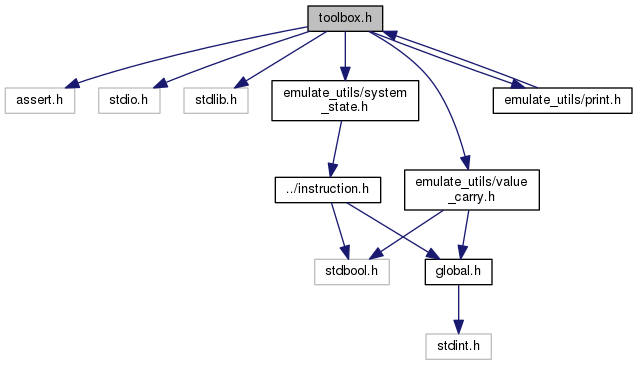
\includegraphics[width=350pt]{toolbox_8h__incl}
\end{center}
\end{figure}
This graph shows which files directly or indirectly include this file\+:\nopagebreak
\begin{figure}[H]
\begin{center}
\leavevmode
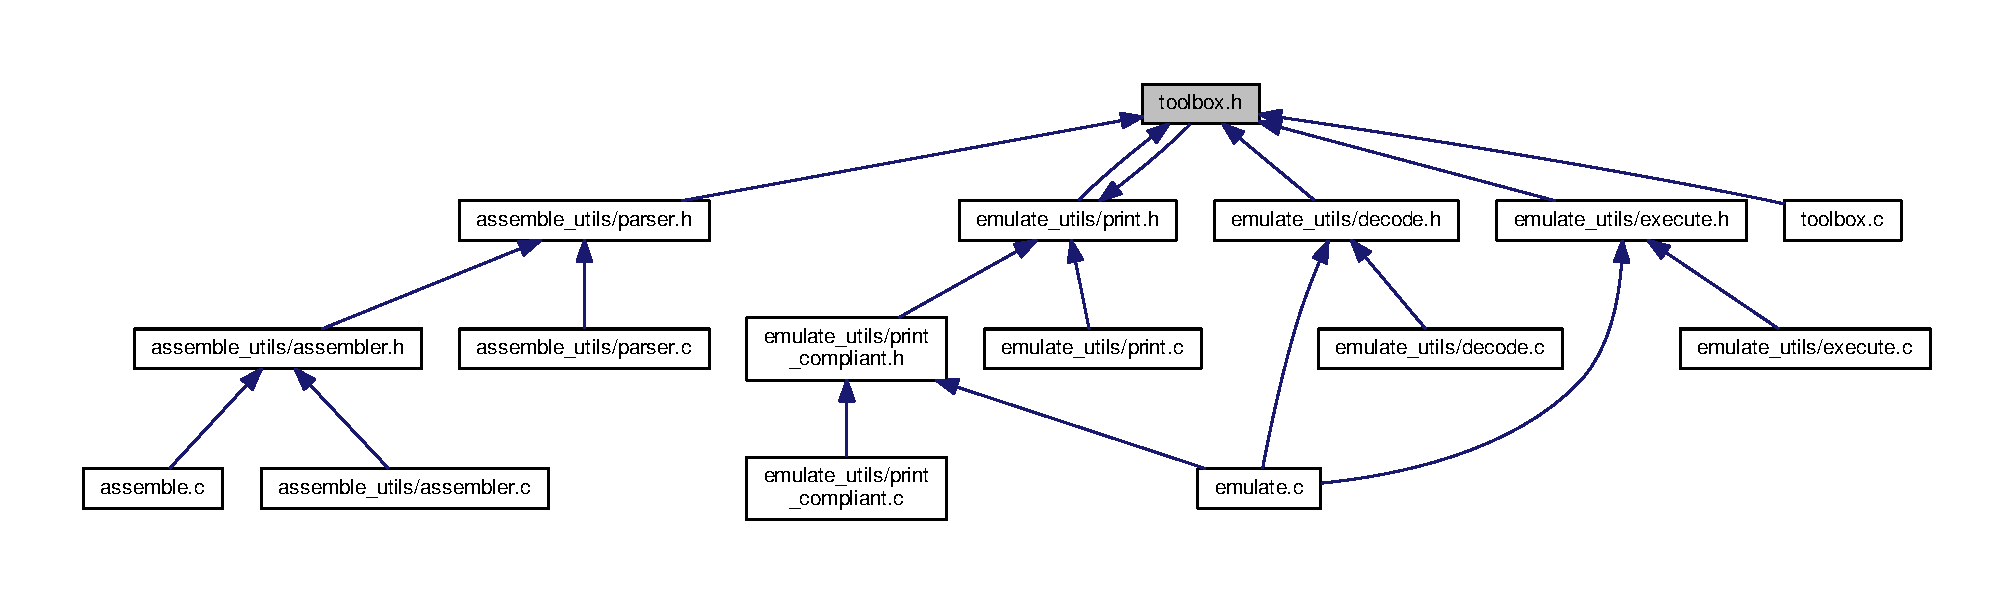
\includegraphics[width=350pt]{toolbox_8h__dep__incl}
\end{center}
\end{figure}
\subsection*{Functions}
\begin{DoxyCompactItemize}
\item 
void \hyperlink{toolbox_8h_a6d650fb79ff7ee7fe331286272a0f794}{load\+\_\+file} (char $\ast$fname, \hyperlink{global_8h_a0661d7d1353e0bca70c64563f635b034}{byte\+\_\+t} $\ast$memory)
\begin{DoxyCompactList}\small\item\em Loads a binary file into the memory. \end{DoxyCompactList}\item 
void \hyperlink{toolbox_8h_a7309491724696785ff2df97b88dbc69d}{exit\+\_\+program} (\hyperlink{structsystem__state__t}{system\+\_\+state\+\_\+t} $\ast$machine)
\begin{DoxyCompactList}\small\item\em Exits gracefully. \end{DoxyCompactList}\item 
\hyperlink{global_8h_a0e7744482eed560726581dae7d3cb8b2}{word\+\_\+t} \hyperlink{toolbox_8h_ae00c97fb61caa5c5a327f53743671ea7}{get\+\_\+word} (\hyperlink{structsystem__state__t}{system\+\_\+state\+\_\+t} $\ast$machine, uint32\+\_\+t mem\+\_\+address)
\begin{DoxyCompactList}\small\item\em Gets a memory word from a given address. \end{DoxyCompactList}\item 
\hyperlink{global_8h_a0e7744482eed560726581dae7d3cb8b2}{word\+\_\+t} \hyperlink{toolbox_8h_a6418bf675c48b3820635a6010b83a159}{get\+\_\+word\+\_\+compliant} (\hyperlink{structsystem__state__t}{system\+\_\+state\+\_\+t} $\ast$machine, \hyperlink{global_8h_a8f4b132f56a25431714862229639be12}{address\+\_\+t} mem\+\_\+address)
\begin{DoxyCompactList}\small\item\em Gets a memory word from a given address (for printing only). \end{DoxyCompactList}\item 
void \hyperlink{toolbox_8h_a17194b5825208d2a4d7c9e266b5fdbc2}{set\+\_\+word} (\hyperlink{structsystem__state__t}{system\+\_\+state\+\_\+t} $\ast$machine, uint32\+\_\+t mem\+\_\+address, \hyperlink{global_8h_a0e7744482eed560726581dae7d3cb8b2}{word\+\_\+t} word)
\begin{DoxyCompactList}\small\item\em Writes a word to memory at a given address. \end{DoxyCompactList}\item 
\hyperlink{global_8h_a0e7744482eed560726581dae7d3cb8b2}{word\+\_\+t} \hyperlink{toolbox_8h_a686137c6e030fbf3387fda07e8eeb085}{negate} (\hyperlink{global_8h_a0e7744482eed560726581dae7d3cb8b2}{word\+\_\+t} value)
\begin{DoxyCompactList}\small\item\em Negates a two\textquotesingle{}s complement value. \end{DoxyCompactList}\item 
bool \hyperlink{toolbox_8h_a0d865a08414b59081c1cbb7787816445}{is\+\_\+negative} (\hyperlink{global_8h_a0e7744482eed560726581dae7d3cb8b2}{word\+\_\+t} value)
\begin{DoxyCompactList}\small\item\em Returns true iff two\textquotesingle{}s complement value is negative. \end{DoxyCompactList}\item 
\hyperlink{global_8h_a0e7744482eed560726581dae7d3cb8b2}{word\+\_\+t} \hyperlink{toolbox_8h_a8c2b56d7b4c74bd125678cf3a1b1f418}{absolute} (\hyperlink{global_8h_a0e7744482eed560726581dae7d3cb8b2}{word\+\_\+t} value)
\begin{DoxyCompactList}\small\item\em Returns absolute two\textquotesingle{}s complement value. \end{DoxyCompactList}\item 
uint32\+\_\+t \hyperlink{toolbox_8h_af5eadf992985ebea2984ce61d8702c4f}{signed\+\_\+to\+\_\+twos\+\_\+complement} (int32\+\_\+t value)
\begin{DoxyCompactList}\small\item\em Returns a two\textquotesingle{}s complement representation for the given value. \end{DoxyCompactList}\item 
long \hyperlink{toolbox_8h_afbd28bd80e4e07eb01e9ea6f6102f637}{twos\+\_\+complement\+\_\+to\+\_\+long} (\hyperlink{global_8h_a0e7744482eed560726581dae7d3cb8b2}{word\+\_\+t} value)
\begin{DoxyCompactList}\small\item\em Converts a signed 2\textquotesingle{}s complement word to a sign long. \end{DoxyCompactList}\item 
\hyperlink{structvalue__carry__t}{value\+\_\+carry\+\_\+t} $\ast$ \hyperlink{toolbox_8h_a519bda814c2b3d1f57613e56de5214b8}{shifter} (\hyperlink{global_8h_a22746cb89e8b2ed0a61876e36446f37f}{shift\+\_\+t} type, \hyperlink{global_8h_a0e7744482eed560726581dae7d3cb8b2}{word\+\_\+t} shift\+\_\+amount, \hyperlink{global_8h_a0e7744482eed560726581dae7d3cb8b2}{word\+\_\+t} value)
\begin{DoxyCompactList}\small\item\em Shifts a value and returns a pointer. \end{DoxyCompactList}\end{DoxyCompactItemize}


\subsection{Detailed Description}
Header file for \hyperlink{toolbox_8c}{toolbox.\+c}. 



\subsection{Function Documentation}
\index{toolbox.\+h@{toolbox.\+h}!absolute@{absolute}}
\index{absolute@{absolute}!toolbox.\+h@{toolbox.\+h}}
\subsubsection[{\texorpdfstring{absolute(word\+\_\+t value)}{absolute(word_t value)}}]{\setlength{\rightskip}{0pt plus 5cm}{\bf word\+\_\+t} absolute (
\begin{DoxyParamCaption}
\item[{{\bf word\+\_\+t}}]{value}
\end{DoxyParamCaption}
)}\hypertarget{toolbox_8h_a8c2b56d7b4c74bd125678cf3a1b1f418}{}\label{toolbox_8h_a8c2b56d7b4c74bd125678cf3a1b1f418}


Returns absolute two\textquotesingle{}s complement value. 


\begin{DoxyParams}{Parameters}
{\em value} & A two\textquotesingle{}s complement word. \\
\hline
\end{DoxyParams}
\begin{DoxyReturn}{Returns}
The absolute value of the provided word in two\textquotesingle{}s complement. 
\end{DoxyReturn}
\index{toolbox.\+h@{toolbox.\+h}!exit\+\_\+program@{exit\+\_\+program}}
\index{exit\+\_\+program@{exit\+\_\+program}!toolbox.\+h@{toolbox.\+h}}
\subsubsection[{\texorpdfstring{exit\+\_\+program(system\+\_\+state\+\_\+t $\ast$machine)}{exit_program(system_state_t *machine)}}]{\setlength{\rightskip}{0pt plus 5cm}void exit\+\_\+program (
\begin{DoxyParamCaption}
\item[{{\bf system\+\_\+state\+\_\+t} $\ast$}]{machine}
\end{DoxyParamCaption}
)}\hypertarget{toolbox_8h_a7309491724696785ff2df97b88dbc69d}{}\label{toolbox_8h_a7309491724696785ff2df97b88dbc69d}


Exits gracefully. 

Prints the current system state, frees allocated memory and exits with a failure. To be used in the case of an error which cannot be recovered from. 
\begin{DoxyParams}{Parameters}
{\em machine} & The current system state. \\
\hline
\end{DoxyParams}
\index{toolbox.\+h@{toolbox.\+h}!get\+\_\+word@{get\+\_\+word}}
\index{get\+\_\+word@{get\+\_\+word}!toolbox.\+h@{toolbox.\+h}}
\subsubsection[{\texorpdfstring{get\+\_\+word(system\+\_\+state\+\_\+t $\ast$machine, uint32\+\_\+t mem\+\_\+address)}{get_word(system_state_t *machine, uint32_t mem_address)}}]{\setlength{\rightskip}{0pt plus 5cm}{\bf word\+\_\+t} get\+\_\+word (
\begin{DoxyParamCaption}
\item[{{\bf system\+\_\+state\+\_\+t} $\ast$}]{machine, }
\item[{uint32\+\_\+t}]{mem\+\_\+address}
\end{DoxyParamCaption}
)}\hypertarget{toolbox_8h_ae00c97fb61caa5c5a327f53743671ea7}{}\label{toolbox_8h_ae00c97fb61caa5c5a327f53743671ea7}


Gets a memory word from a given address. 


\begin{DoxyItemize}
\item If G\+P\+IO access adddress is read, prints a message to stdout.
\item If another out of bounds address is read, prints an error. 
\begin{DoxyParams}{Parameters}
{\em machine} & The current system state. \\
\hline
{\em mem\+\_\+address} & The memory address to be read from. \\
\hline
\end{DoxyParams}
\begin{DoxyReturn}{Returns}
The word at the given memory address in the current system state. 
\end{DoxyReturn}

\end{DoxyItemize}\index{toolbox.\+h@{toolbox.\+h}!get\+\_\+word\+\_\+compliant@{get\+\_\+word\+\_\+compliant}}
\index{get\+\_\+word\+\_\+compliant@{get\+\_\+word\+\_\+compliant}!toolbox.\+h@{toolbox.\+h}}
\subsubsection[{\texorpdfstring{get\+\_\+word\+\_\+compliant(system\+\_\+state\+\_\+t $\ast$machine, address\+\_\+t mem\+\_\+address)}{get_word_compliant(system_state_t *machine, address_t mem_address)}}]{\setlength{\rightskip}{0pt plus 5cm}{\bf word\+\_\+t} get\+\_\+word\+\_\+compliant (
\begin{DoxyParamCaption}
\item[{{\bf system\+\_\+state\+\_\+t} $\ast$}]{machine, }
\item[{{\bf address\+\_\+t}}]{mem\+\_\+address}
\end{DoxyParamCaption}
)}\hypertarget{toolbox_8h_a6418bf675c48b3820635a6010b83a159}{}\label{toolbox_8h_a6418bf675c48b3820635a6010b83a159}


Gets a memory word from a given address (for printing only). 

For use in compliant printing. Gets the word in little endian order. 
\begin{DoxyParams}{Parameters}
{\em machine} & The current system state. \\
\hline
{\em mem\+\_\+address} & The memory address to be read from. \\
\hline
\end{DoxyParams}
\begin{DoxyReturn}{Returns}
The word at the given memory address in the current system state. 
\end{DoxyReturn}
\index{toolbox.\+h@{toolbox.\+h}!is\+\_\+negative@{is\+\_\+negative}}
\index{is\+\_\+negative@{is\+\_\+negative}!toolbox.\+h@{toolbox.\+h}}
\subsubsection[{\texorpdfstring{is\+\_\+negative(word\+\_\+t value)}{is_negative(word_t value)}}]{\setlength{\rightskip}{0pt plus 5cm}bool is\+\_\+negative (
\begin{DoxyParamCaption}
\item[{{\bf word\+\_\+t}}]{value}
\end{DoxyParamCaption}
)}\hypertarget{toolbox_8h_a0d865a08414b59081c1cbb7787816445}{}\label{toolbox_8h_a0d865a08414b59081c1cbb7787816445}


Returns true iff two\textquotesingle{}s complement value is negative. 


\begin{DoxyParams}{Parameters}
{\em value} & A two\textquotesingle{}s complement word to check sign of. \\
\hline
\end{DoxyParams}
\begin{DoxyReturn}{Returns}
True iff provided value is negative in two\textquotesingle{}s complement. 
\end{DoxyReturn}
\index{toolbox.\+h@{toolbox.\+h}!load\+\_\+file@{load\+\_\+file}}
\index{load\+\_\+file@{load\+\_\+file}!toolbox.\+h@{toolbox.\+h}}
\subsubsection[{\texorpdfstring{load\+\_\+file(char $\ast$fname, byte\+\_\+t $\ast$memory)}{load_file(char *fname, byte_t *memory)}}]{\setlength{\rightskip}{0pt plus 5cm}void load\+\_\+file (
\begin{DoxyParamCaption}
\item[{char $\ast$}]{fname, }
\item[{{\bf byte\+\_\+t} $\ast$}]{memory}
\end{DoxyParamCaption}
)}\hypertarget{toolbox_8h_a6d650fb79ff7ee7fe331286272a0f794}{}\label{toolbox_8h_a6d650fb79ff7ee7fe331286272a0f794}


Loads a binary file into the memory. 

Writes the contents of the provided binary object code file to the memory, starting at the provided location. Returns an error message and exits if the file cannot be opened or cannot be read. 
\begin{DoxyParams}{Parameters}
{\em fname} & The filename containing object code to be loaded. \\
\hline
{\em memory} & A pointer to the first byte of memory to be written to. \\
\hline
\end{DoxyParams}
\index{toolbox.\+h@{toolbox.\+h}!negate@{negate}}
\index{negate@{negate}!toolbox.\+h@{toolbox.\+h}}
\subsubsection[{\texorpdfstring{negate(word\+\_\+t value)}{negate(word_t value)}}]{\setlength{\rightskip}{0pt plus 5cm}{\bf word\+\_\+t} negate (
\begin{DoxyParamCaption}
\item[{{\bf word\+\_\+t}}]{value}
\end{DoxyParamCaption}
)}\hypertarget{toolbox_8h_a686137c6e030fbf3387fda07e8eeb085}{}\label{toolbox_8h_a686137c6e030fbf3387fda07e8eeb085}


Negates a two\textquotesingle{}s complement value. 


\begin{DoxyParams}{Parameters}
{\em value} & The word to be negated. \\
\hline
\end{DoxyParams}
\begin{DoxyReturn}{Returns}
The negated word. 
\end{DoxyReturn}
\index{toolbox.\+h@{toolbox.\+h}!set\+\_\+word@{set\+\_\+word}}
\index{set\+\_\+word@{set\+\_\+word}!toolbox.\+h@{toolbox.\+h}}
\subsubsection[{\texorpdfstring{set\+\_\+word(system\+\_\+state\+\_\+t $\ast$machine, uint32\+\_\+t mem\+\_\+address, word\+\_\+t word)}{set_word(system_state_t *machine, uint32_t mem_address, word_t word)}}]{\setlength{\rightskip}{0pt plus 5cm}void set\+\_\+word (
\begin{DoxyParamCaption}
\item[{{\bf system\+\_\+state\+\_\+t} $\ast$}]{machine, }
\item[{uint32\+\_\+t}]{mem\+\_\+address, }
\item[{{\bf word\+\_\+t}}]{word}
\end{DoxyParamCaption}
)}\hypertarget{toolbox_8h_a17194b5825208d2a4d7c9e266b5fdbc2}{}\label{toolbox_8h_a17194b5825208d2a4d7c9e266b5fdbc2}


Writes a word to memory at a given address. 


\begin{DoxyItemize}
\item If G\+P\+IO access adddress is written to, prints a message to stdout.
\item If G\+P\+IO clear or set adddress is written to, prints a message to stdout.
\item If another out of bounds address is read, prints an error. 
\begin{DoxyParams}{Parameters}
{\em machine} & The current system state. \\
\hline
{\em mem\+\_\+address} & The memory address to write to. \\
\hline
{\em word} & The word to write to memory. \\
\hline
\end{DoxyParams}

\end{DoxyItemize}\index{toolbox.\+h@{toolbox.\+h}!shifter@{shifter}}
\index{shifter@{shifter}!toolbox.\+h@{toolbox.\+h}}
\subsubsection[{\texorpdfstring{shifter(shift\+\_\+t type, word\+\_\+t shift\+\_\+amount, word\+\_\+t value)}{shifter(shift_t type, word_t shift_amount, word_t value)}}]{\setlength{\rightskip}{0pt plus 5cm}{\bf value\+\_\+carry\+\_\+t}$\ast$ shifter (
\begin{DoxyParamCaption}
\item[{{\bf shift\+\_\+t}}]{type, }
\item[{{\bf word\+\_\+t}}]{shift\+\_\+amount, }
\item[{{\bf word\+\_\+t}}]{value}
\end{DoxyParamCaption}
)}\hypertarget{toolbox_8h_a519bda814c2b3d1f57613e56de5214b8}{}\label{toolbox_8h_a519bda814c2b3d1f57613e56de5214b8}


Shifts a value and returns a pointer. 


\begin{DoxyParams}{Parameters}
{\em type} & The type of shift to use. \\
\hline
{\em shift\+\_\+amount} & The amount to shift by. \\
\hline
{\em value} & The value to shift. \\
\hline
\end{DoxyParams}
\begin{DoxyReturn}{Returns}
The pointer to the shifted value. 
\end{DoxyReturn}
\index{toolbox.\+h@{toolbox.\+h}!signed\+\_\+to\+\_\+twos\+\_\+complement@{signed\+\_\+to\+\_\+twos\+\_\+complement}}
\index{signed\+\_\+to\+\_\+twos\+\_\+complement@{signed\+\_\+to\+\_\+twos\+\_\+complement}!toolbox.\+h@{toolbox.\+h}}
\subsubsection[{\texorpdfstring{signed\+\_\+to\+\_\+twos\+\_\+complement(int32\+\_\+t value)}{signed_to_twos_complement(int32_t value)}}]{\setlength{\rightskip}{0pt plus 5cm}uint32\+\_\+t signed\+\_\+to\+\_\+twos\+\_\+complement (
\begin{DoxyParamCaption}
\item[{int32\+\_\+t}]{value}
\end{DoxyParamCaption}
)}\hypertarget{toolbox_8h_af5eadf992985ebea2984ce61d8702c4f}{}\label{toolbox_8h_af5eadf992985ebea2984ce61d8702c4f}


Returns a two\textquotesingle{}s complement representation for the given value. 


\begin{DoxyParams}{Parameters}
{\em value} & The value to convert. \\
\hline
\end{DoxyParams}
\begin{DoxyReturn}{Returns}
A 32-\/bit two\textquotesingle{}s complement representation. 
\end{DoxyReturn}
\index{toolbox.\+h@{toolbox.\+h}!twos\+\_\+complement\+\_\+to\+\_\+long@{twos\+\_\+complement\+\_\+to\+\_\+long}}
\index{twos\+\_\+complement\+\_\+to\+\_\+long@{twos\+\_\+complement\+\_\+to\+\_\+long}!toolbox.\+h@{toolbox.\+h}}
\subsubsection[{\texorpdfstring{twos\+\_\+complement\+\_\+to\+\_\+long(word\+\_\+t value)}{twos_complement_to_long(word_t value)}}]{\setlength{\rightskip}{0pt plus 5cm}long twos\+\_\+complement\+\_\+to\+\_\+long (
\begin{DoxyParamCaption}
\item[{{\bf word\+\_\+t}}]{value}
\end{DoxyParamCaption}
)}\hypertarget{toolbox_8h_afbd28bd80e4e07eb01e9ea6f6102f637}{}\label{toolbox_8h_afbd28bd80e4e07eb01e9ea6f6102f637}


Converts a signed 2\textquotesingle{}s complement word to a sign long. 


\begin{DoxyParams}{Parameters}
{\em value} & The signed 2\textquotesingle{}s complement word to convert. \\
\hline
\end{DoxyParams}
\begin{DoxyReturn}{Returns}
The signed long representation of the word. 
\end{DoxyReturn}

\hypertarget{value__carry_8h}{}\section{emulate\+\_\+utils/value\+\_\+carry.h File Reference}
\label{value__carry_8h}\index{emulate\+\_\+utils/value\+\_\+carry.\+h@{emulate\+\_\+utils/value\+\_\+carry.\+h}}


A header to define the \hyperlink{structvalue__carry__t}{value\+\_\+carry\+\_\+t} type.  


{\ttfamily \#include $<$stdbool.\+h$>$}\\*
{\ttfamily \#include \char`\"{}../global.\+h\char`\"{}}\\*
Include dependency graph for value\+\_\+carry.\+h\+:\nopagebreak
\begin{figure}[H]
\begin{center}
\leavevmode
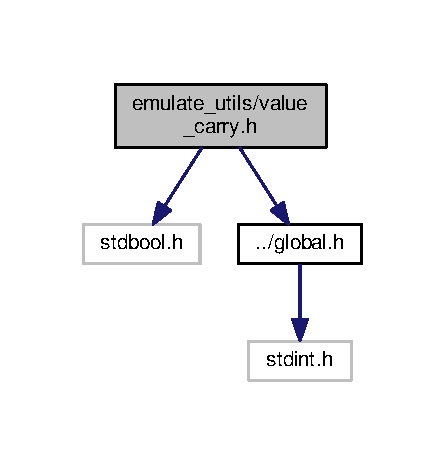
\includegraphics[width=214pt]{value__carry_8h__incl}
\end{center}
\end{figure}
This graph shows which files directly or indirectly include this file\+:\nopagebreak
\begin{figure}[H]
\begin{center}
\leavevmode
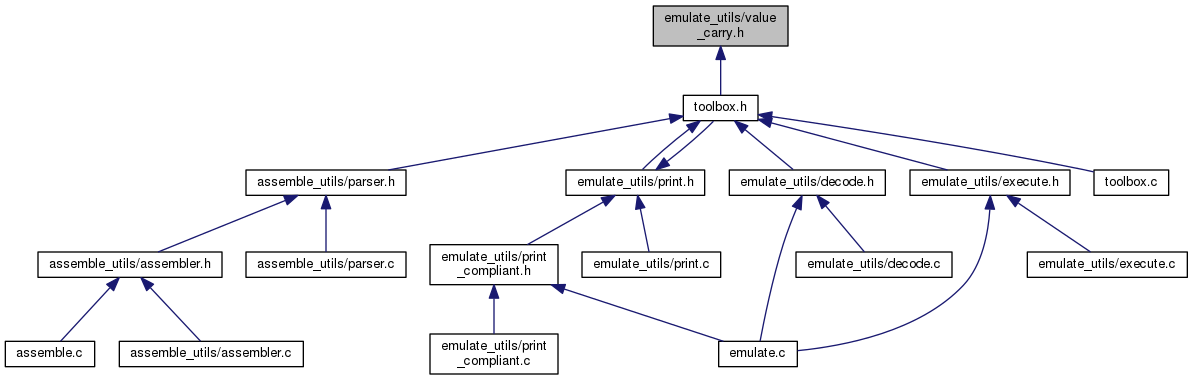
\includegraphics[width=350pt]{value__carry_8h__dep__incl}
\end{center}
\end{figure}
\subsection*{Data Structures}
\begin{DoxyCompactItemize}
\item 
struct \hyperlink{structvalue__carry__t}{value\+\_\+carry\+\_\+t}
\begin{DoxyCompactList}\small\item\em A struct that has a value and a carry. \end{DoxyCompactList}\end{DoxyCompactItemize}


\subsection{Detailed Description}
A header to define the \hyperlink{structvalue__carry__t}{value\+\_\+carry\+\_\+t} type. 


%--- End generated contents ---

% Index
\backmatter
\newpage
\phantomsection
\clearemptydoublepage
\addcontentsline{toc}{chapter}{Index}
\printindex

\end{document}
